% =======================================================
\section{Experiments}
\label{sec:experiments}
% =======================================================
\subsection{E1--E2: In-distribution accuracy under noise and undersampling}\label{sec:e1e2}
\paragraph{Setting.}
Test images are 200 MNIST digits and all hyper-parameters are tuned on 100 separate validation images (Section~\ref{sec:settings}). The
noise sweep fixes 20 projection angles and varies the measurement noise $\sigma\in\{0,0.01,0.05,0.1,0.2\}$; the angle sweep fixes
$\sigma=0.05$ and uses $5,10,20,40,90$ angles. Each cell is one noise realisation. Tables~\ref{tab:e1e2} and~\ref{tab:e1e2gap} first use data generated with the reconstruction
operator itself (``inverse crime''), because this is the setting of the original study; Table~\ref{tab:e1e2gap} then repeats the PnP--TV
comparison with data simulated on a finer grid (bicubic, factor~5; the default crime-free setting, Section~\ref{sec:crime-results}).
Two total-variation baselines are reported: \emph{TV-ADMM} is the unconstrained ADMM solver used throughout Stages~1--2, and
\emph{TV-box} is the same functional solved with the constraint $0\le x\le1$ by Chambolle--Pock (1000 iterations, $\lambda$ re-tuned on the validation images).
TV-box is the fairer comparison, because the PnP iterates are clipped to $[0,1]$ at every iteration; it is a control added after the main experiments (E2b), and the other
Stage~1--2 experiments (E3, E5, E7, E10 and the Stage~2 dose sweep) were run against TV-ADMM only.

\begin{table}[htbp]
\centering\small\setlength{\tabcolsep}{5pt}
\caption{Test PSNR (dB), mean over 200 images, data generated with the reconstruction operator (inverse crime). Bold: highest mean in the row (not a significance statement; see Table~\ref{tab:e1e2gap} for paired intervals).
$\dagger$: the TV-box optimum lies below the initial $\lambda$ grid ($\lambda_{\mathrm{norm}}=3.7\times10^{-7}$, i.e.\ almost no regularisation), so $42.5$\,dB
is a data-model artefact and should not be read as a property of TV.}\label{tab:e1e2}
\begin{tabular}{lcccccc}
\toprule
Condition & FBP & Tikhonov & TV-ADMM & TV-box & PnP-DnCNN \\
\midrule
$\sigma{=}0$, 20 angles     & 24.2 & 28.9 & 36.0 & \textbf{42.5}$^\dagger$ & 29.6 \\
$\sigma{=}0.01$, 20 angles  & 23.1 & 24.1 & 29.0 & \textbf{29.8} & 29.1 \\
$\sigma{=}0.05$, 20 angles  & 15.5 & 17.1 & 20.1 & 20.7 & \textbf{24.0} \\
$\sigma{=}0.1$, 20 angles   & 10.4 & 14.7 & 16.9 & 17.2 & \textbf{19.9} \\
$\sigma{=}0.2$, 20 angles   & 6.6  & 12.9 & 14.3 & 14.6 & \textbf{15.3} \\
\midrule
5 angles, $\sigma{=}0.05$   & 9.1  & 14.2 & 15.5 & 16.5 & \textbf{17.7} \\
10 angles, $\sigma{=}0.05$  & 12.1 & 15.9 & 18.4 & 18.9 & \textbf{21.4} \\
40 angles, $\sigma{=}0.05$  & 18.1 & 18.2 & 21.8 & 22.4 & \textbf{25.6} \\
90 angles, $\sigma{=}0.05$  & 20.6 & 20.0 & 24.1 & 24.6 & \textbf{27.1} \\
\bottomrule
\end{tabular}
\end{table}

\begin{table}[htbp]
\centering\small\setlength{\tabcolsep}{4pt}
\caption{PnP$-$TV PSNR gap (dB) with 95\% bootstrap intervals over the 200 test images; positive means PnP is better. Left: data generated with the reconstruction operator (the PSNR values of Table~\ref{tab:e1e2}).
Right: data simulated on a finer grid, which removes the inverse crime. Hyper-parameters are re-tuned for each data model. $\dagger$: see Table~\ref{tab:e1e2}.}\label{tab:e1e2gap}
\begin{tabular}{lcccc}
\toprule
 & \multicolumn{2}{c}{Inverse crime} & \multicolumn{2}{c}{Crime-free (bicubic)}\\
\cmidrule(lr){2-3}\cmidrule(lr){4-5}
Condition & vs TV-ADMM & vs TV-box & vs TV-ADMM & vs TV-box \\
\midrule
$\sigma{=}0$, 20 angles    & $-6.43$ [$-6.70,-6.18$] & $-12.93$ [$-13.30,-12.57$]$^\dagger$ & $-3.29$ [$-3.47,-3.10$] & $-5.13$ [$-5.32,-4.94$] \\
$\sigma{=}0.01$, 20 angles & $+0.07$ [$-0.07,+0.21$] & $-0.75$ [$-0.89,-0.60$] & $+1.02$ [$+0.87,+1.16$] & $+0.35$ [$+0.21,+0.49$] \\
$\sigma{=}0.05$, 20 angles & $+3.86$ [$+3.70,+4.02$] & $+3.33$ [$+3.19,+3.47$] & $+4.02$ [$+3.85,+4.18$] & $+3.48$ [$+3.34,+3.63$] \\
$\sigma{=}0.1$, 20 angles  & $+3.01$ [$+2.79,+3.24$] & $+2.65$ [$+2.43,+2.88$] & $+3.10$ [$+2.88,+3.33$] & $+2.73$ [$+2.51,+2.96$] \\
$\sigma{=}0.2$, 20 angles  & $+1.03$ [$+0.78,+1.29$] & $+0.65$ [$+0.40,+0.89$] & $+1.08$ [$+0.83,+1.33$] & $+0.69$ [$+0.45,+0.93$] \\
\midrule
5 angles, $\sigma{=}0.05$  & $+2.13$ [$+1.86,+2.41$] & $+1.14$ [$+0.90,+1.39$] & $+2.36$ [$+2.07,+2.64$] & $+1.35$ [$+1.10,+1.61$] \\
10 angles, $\sigma{=}0.05$ & $+3.03$ [$+2.81,+3.26$] & $+2.51$ [$+2.28,+2.75$] & $+3.29$ [$+3.09,+3.50$] & $+2.77$ [$+2.56,+2.98$] \\
40 angles, $\sigma{=}0.05$ & $+3.83$ [$+3.69,+3.97$] & $+3.26$ [$+3.13,+3.39$] & $+3.97$ [$+3.82,+4.11$] & $+3.39$ [$+3.26,+3.52$] \\
90 angles, $\sigma{=}0.05$ & $+3.04$ [$+2.90,+3.18$] & $+2.57$ [$+2.44,+2.69$] & $+3.24$ [$+3.10,+3.39$] & $+2.79$ [$+2.67,+2.91$] \\
\bottomrule
\end{tabular}
\end{table}

\begin{figure}[htbp]
\centering
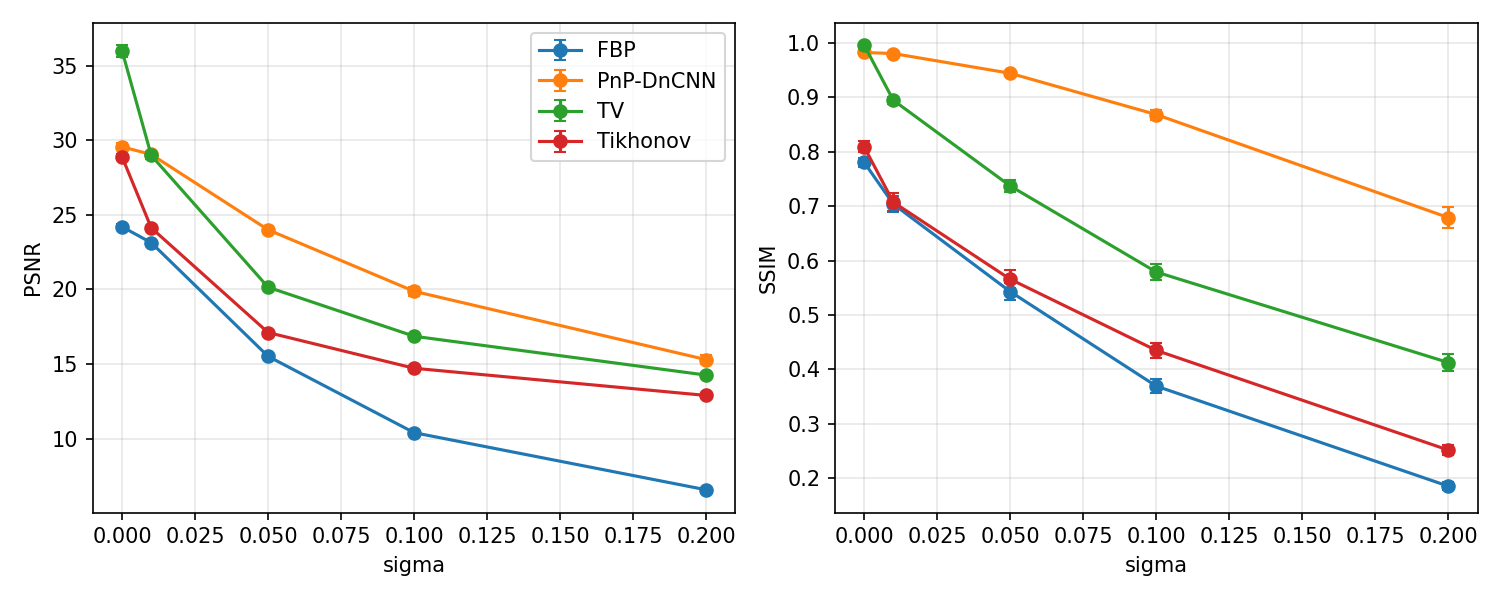
\includegraphics[width=0.95\textwidth]{figures/comparison_noise.png}
\caption{Reconstruction accuracy (PSNR, left; SSIM, right) against the measurement noise $\sigma$ at 20 projection angles, inverse-crime data, TV-ADMM as the TV baseline. At $\sigma=0$ TV is clearly best in PSNR; at $\sigma=0.01$ TV and PnP-DnCNN are within noise of each other in PSNR (Table~\ref{tab:e1e2gap}), while PnP has the higher SSIM; for $\sigma\ge0.05$ PnP-DnCNN is best in both. Error bars are the mean $\pm1.96$ standard errors over 200 test images and reflect image-to-image variability only, not tuning or training variability.}
\label{fig:comparison_noise}
\end{figure}

\begin{figure}[htbp]
\centering
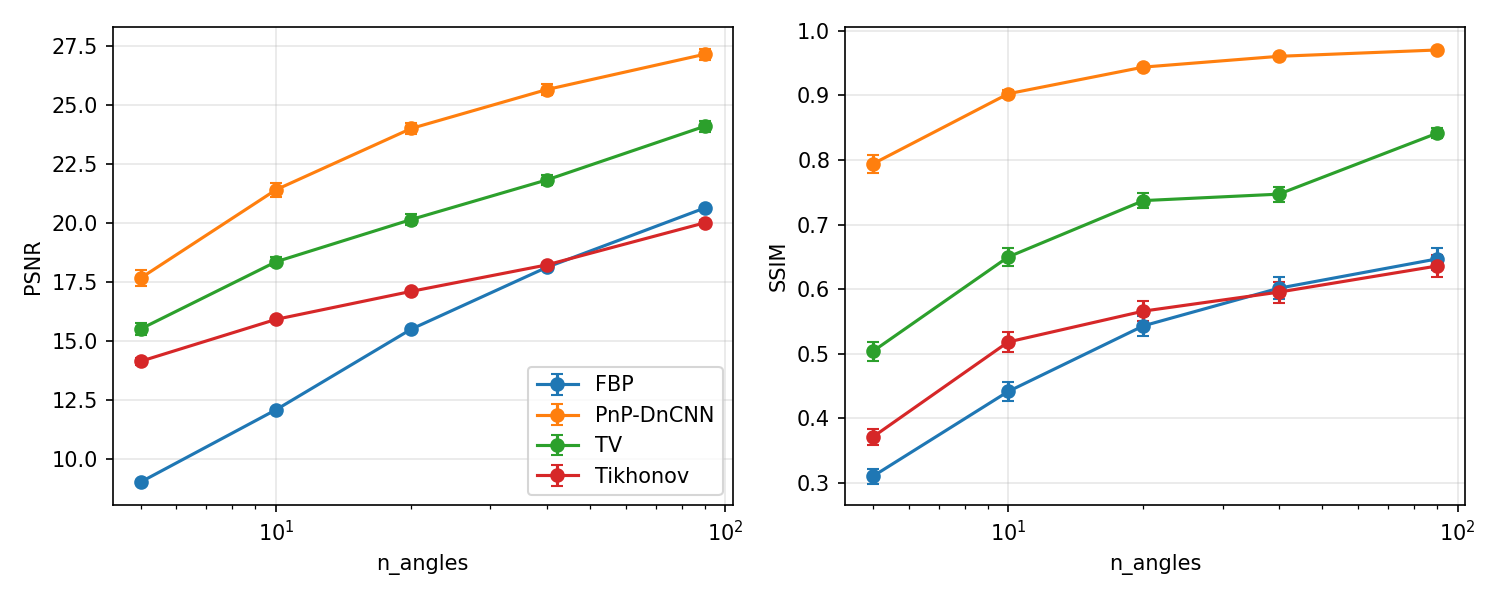
\includegraphics[width=0.95\textwidth]{figures/comparison_angles.png}
\caption{Reconstruction accuracy (PSNR, left; SSIM, right) against the number of projection angles at $\sigma=0.05$ (logarithmic axis), inverse-crime data, TV-ADMM as the TV baseline. PnP-DnCNN is best at every angle count tested. Error bars as in Figure~\ref{fig:comparison_noise}.}
\label{fig:comparison_angles}
\end{figure}

\begin{figure}[htbp]
\centering
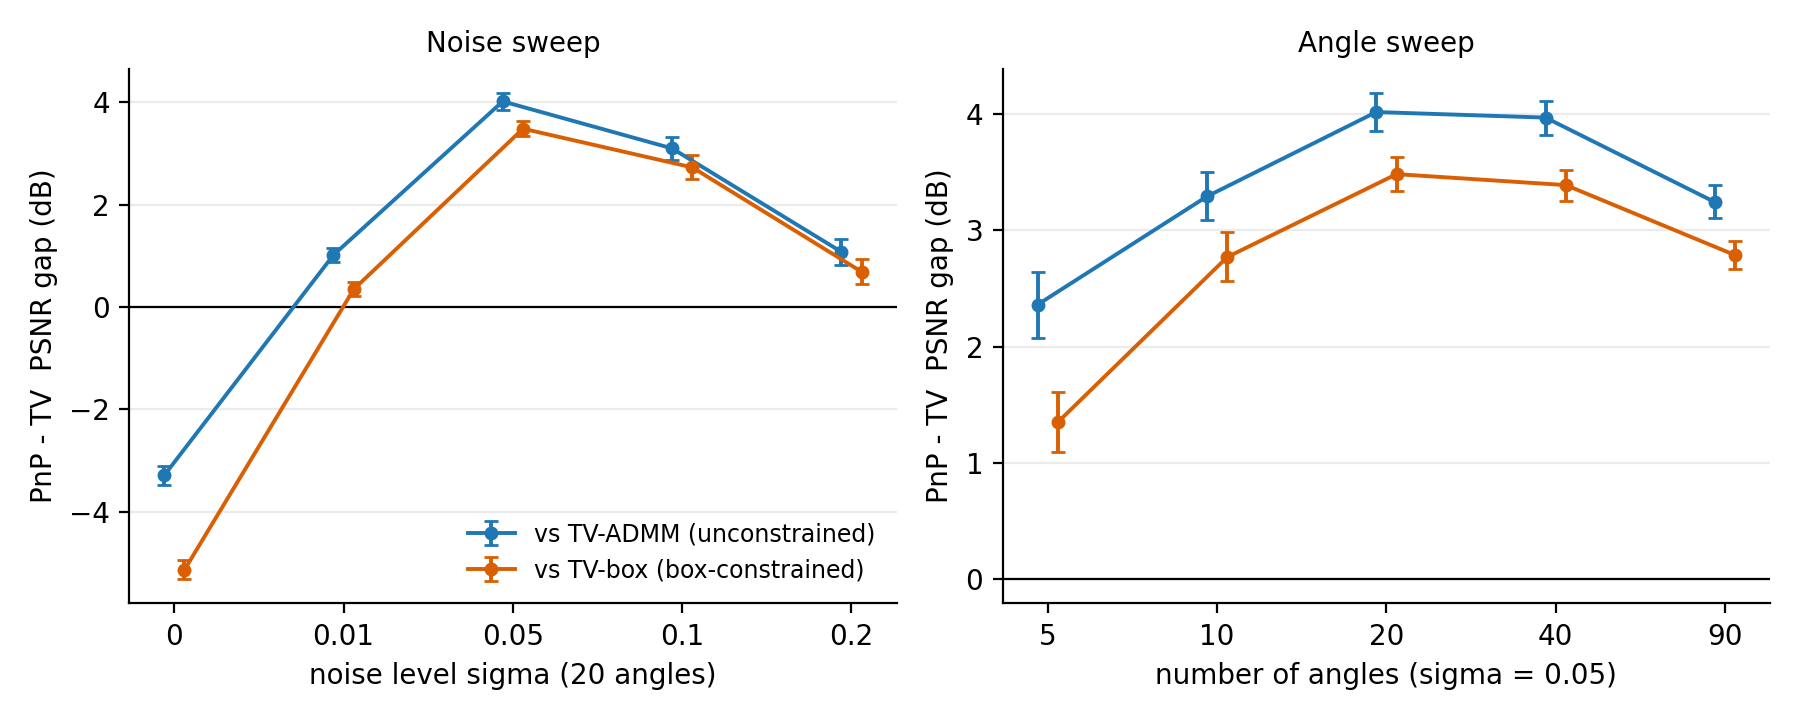
\includegraphics[width=0.95\textwidth]{figures/fig_e1e2_gap.png}
\caption{PnP$-$TV PSNR gap on crime-free (bicubic) data against the unconstrained TV-ADMM and the box-constrained TV-box. Bars are 95\% bootstrap intervals over 200 images. The box constraint lowers the PnP advantage by $0.4$--$1.0$\,dB at $\sigma\ge0.05$ and, in the angle sweep, most at 5 angles; it does not change the sign anywhere except at $\sigma=0.01$ on inverse-crime data (Table~\ref{tab:e1e2gap}).}
\label{fig:e1e2gap}
\end{figure}

\paragraph{Results.}
\emph{(i) Where the learned prior wins.} For $\sigma\ge0.05$ PnP-DnCNN has the highest PSNR at every angle count and noise level tested, and the gap
over TV is significantly positive against both TV variants and on both data models (Table~\ref{tab:e1e2gap}). The gap is largest at $\sigma=0.05$ with 20--40 angles:
$+3.8$ to $+3.9$\,dB against TV-ADMM, but $+3.3$\,dB against TV-box on inverse-crime data and $+3.4$ to $+3.5$\,dB on crime-free data. We take the box-constrained, crime-free value as the headline
($\approx3.5$\,dB for this denoiser; $3.4$\,dB averaged over three independently trained denoisers in E8). Against TV-ADMM, PnP has the higher PSNR in 100\% of the 200 images at $\sigma=0.05$ with 20, 40 and 90 angles, in 96\% at $\sigma=0.1$, but only
in 68\% at $\sigma=0.2$ and 87\% at 5 angles, where the average gap is small ($+1.0$ and $+2.1$\,dB). Against TV-box the gap shrinks fastest in the hardest regimes: from $+2.1$ to $+1.1$\,dB at 5 angles and
from $+1.03$ to $+0.65$\,dB at $\sigma=0.2$ (inverse-crime data).

\emph{(ii) SSIM.} The SSIM gain is larger than the PSNR gain suggests (TV-ADMM $0.74\to$ PnP $0.94$ at $\sigma=0.05$ with 20 angles; $0.50\to0.79$ at 5 angles; $0.41\to0.68$ at $\sigma=0.2$) and PnP has the higher SSIM, significantly so (paired Wilcoxon), in every condition except $\sigma=0$, where TV is significantly higher ($0.996$ vs.\ $0.982$). We did not compute SSIM for TV-box. SSIM is later shown to be lower for PnP on real CT (Stage~3); we attribute the high SSIM here to the match between
the denoiser's training distribution and the test digits, but did not test this.

\emph{(iii) The noise-free and low-noise end depends on the data model and the TV solver.} At $\sigma=0$ the learned prior is below TV in every variant ($-6.4$\,dB on inverse-crime data, $-3.3$\,dB crime-free against TV-ADMM; larger still against TV-box).
At $\sigma=0.01$ the sign of the PnP--TV gap changes with these choices: not distinguishable from zero against TV-ADMM on inverse-crime data ($+0.07$\,dB), $-0.75$\,dB against TV-box on the same data, and $+0.35$\,dB against TV-box on crime-free data.
No claim about PnP versus TV at $\sigma\le0.01$ should therefore be made from E1--E2 alone; Section~\ref{sec:crime-results} analyses the data-model dependence.

\emph{(iv) Classical baselines.} TV (either variant) is the best classical method in every condition, and Tikhonov is above FBP except at 90 angles (Table~\ref{tab:e1e2}). A possible reason for TV's advantage is that digit images are close to piecewise constant; we did not test this.

\paragraph{Caveats.}
(a)~Each cell uses one noise realisation, a single denoiser and one tuning run; the intervals in Table~\ref{tab:e1e2gap} describe the variability across test images only. The only measure of
training variability is E8 (three denoisers), where the in-distribution gap varies by $0.03$\,dB between seeds, small compared with the gaps above.
(b)~PnP has two tuned parameters (denoiser level $\sigma_d$ and iteration count $k$, $5\le k\le100$ across conditions) against one for TV, and early stopping is itself a regulariser. The TV baselines are run to convergence (1000 iterations for TV-box; 100 for TV-ADMM), so the comparison is between a tuned few-iteration PnP and a converged TV; the inclusion of TV-box addresses the box constraint but not the difference in tuning degrees of freedom.
(c)~All numbers are for $28\times28$ digits whose training distribution matches the test distribution by construction; what happens when it does not is the subject of E4 and E8.

\begin{figure}[htbp]
\centering
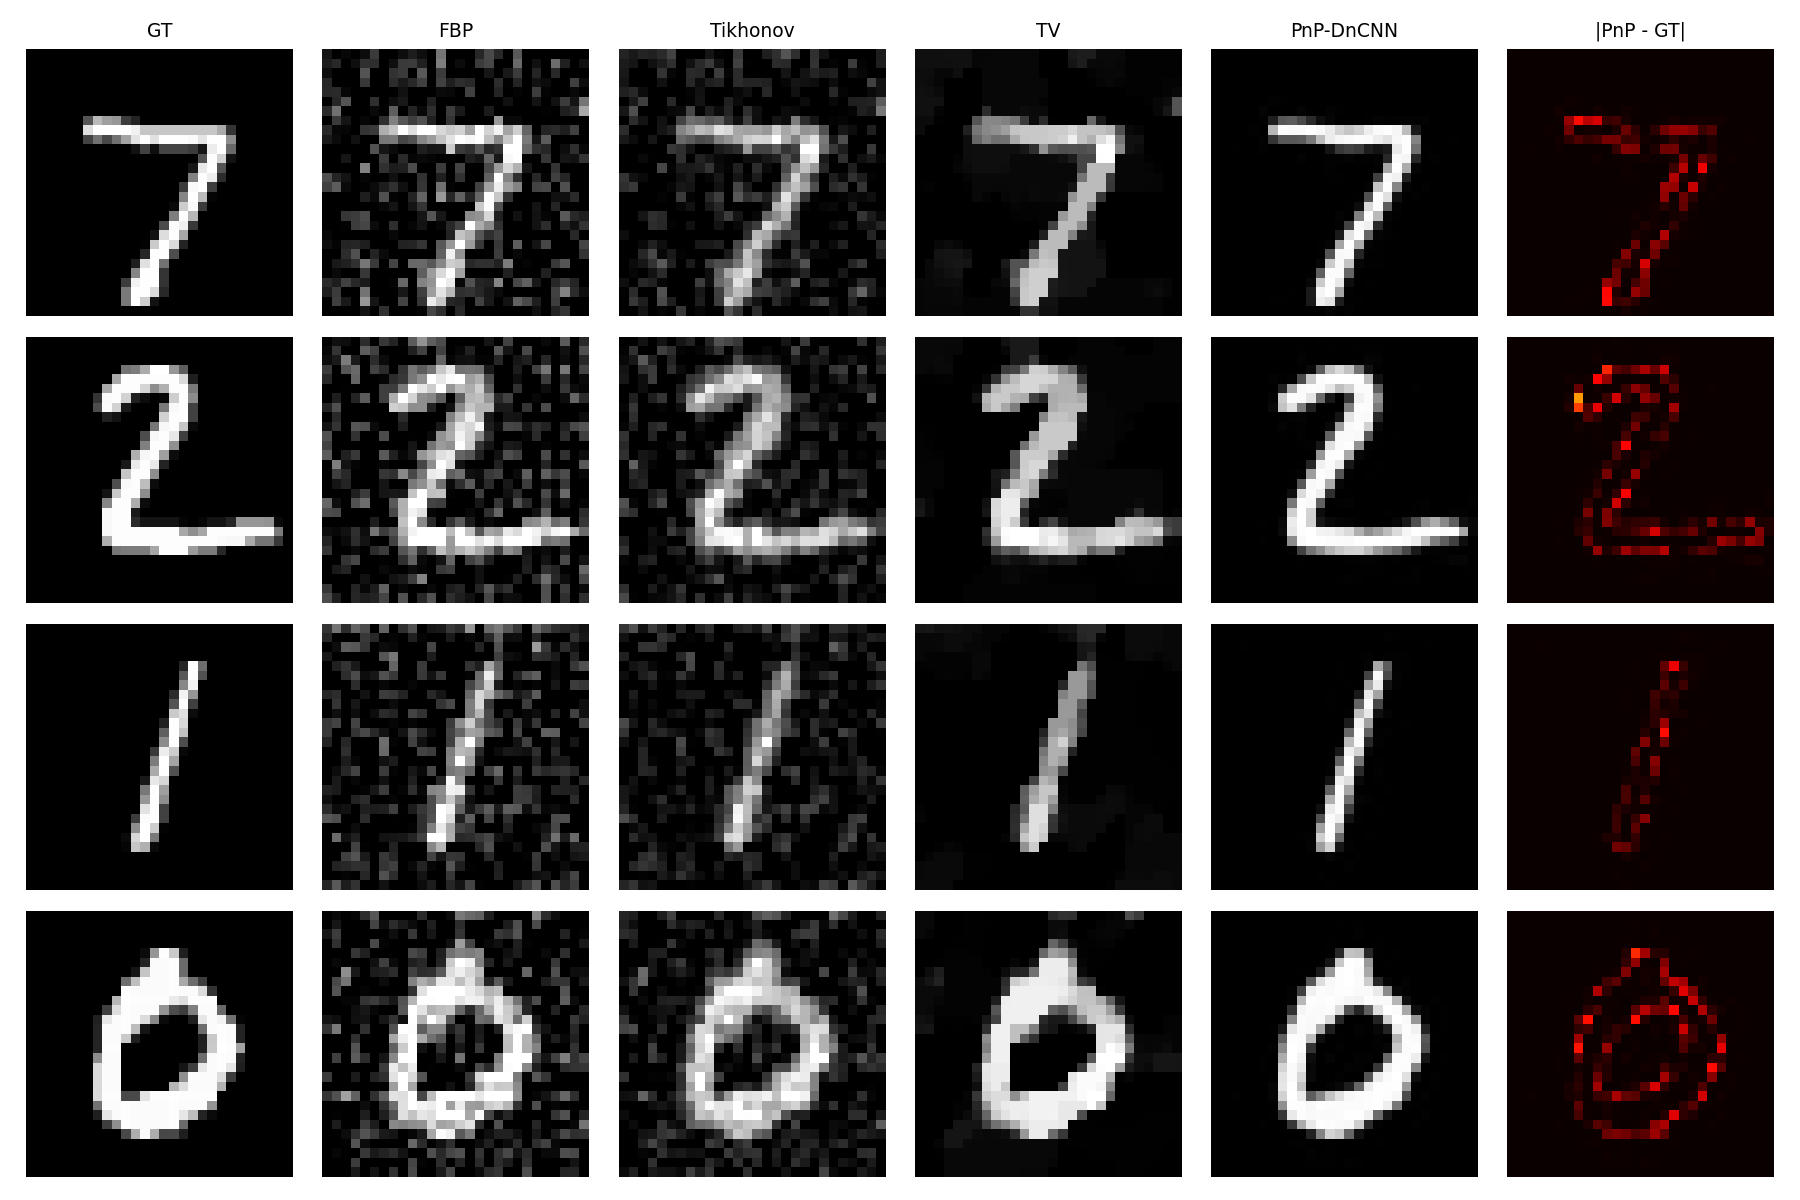
\includegraphics[width=0.95\textwidth]{figures/fig_recon_grid.png}
\caption{In-distribution reconstructions at $\sigma=0.05$, 20 angles (inverse-crime data, one noise draw). Rows are the first four test images (no selection). Columns: ground truth, FBP, Tikhonov, TV-ADMM, PnP-DnCNN and the absolute error $|\hat{x}_{\mathrm{PnP}}-x|$ (brighter is larger). FBP and Tikhonov retain visible noise; TV-ADMM gives flat regions with reduced stroke intensity; PnP-DnCNN is visually closest to the ground truth. The error maps show the residual concentrated along stroke boundaries. A TV-box column and per-image PSNR values are not shown.}
\label{fig:recon_grid}
\end{figure}


\subsection{E3: Forward-model mismatch}\label{sec:e3}
\paragraph{Setting.}
Measurements are generated with the true 20-angle operator at $\sigma=0.05$ (inverse-crime data, 200 test digits), and the reconstruction uses an operator whose projection angles are
perturbed by $\delta\in\{0,0.5,1,2,4\}^\circ$ (the angular spacing is $9^\circ$). Two perturbations are used: a \emph{constant offset}, $\theta_j\to\theta_j+\delta$, and \emph{per-angle jitter},
$\theta_j\to\theta_j+\delta\,\varepsilon_j$ with $\varepsilon_j\sim\mathcal{N}(0,1)$, so that $\delta$ is the standard deviation, not a bound. One jitter vector is drawn per level (fixed seed) and shared by all images and methods.
All hyper-parameters are frozen at their values for the nominal, matched operator (TV-ADMM $\lambda=5.6\times10^{-3}$; PnP $\sigma_d=0.1$, $k=5$; Tikhonov $\lambda=1.8\times10^{-2}$) and are not re-tuned under mismatch.
The TV baseline is the unconstrained TV-ADMM; E3 was not repeated with TV-box.

\begin{table}[htbp]
\centering\small\setlength{\tabcolsep}{4pt}
\caption{Test PSNR (dB) under forward-model mismatch with hyper-parameters frozen at their nominal values, and the PnP$-$TV gap (mean $\pm1.96$ standard errors of the paired per-image difference, 200 images).
PnP has the higher PSNR in 100\% of the images in every row except $\delta=4^\circ$ (96\% for the offset, 99\% for the jitter).}
\label{tab:e3}
\begin{tabular}{lcccccc}
\toprule
 & \multicolumn{3}{c}{Constant offset} & \multicolumn{3}{c}{Per-angle jitter ($\delta$ = s.d.)}\\
\cmidrule(lr){2-4}\cmidrule(lr){5-7}
$\delta$ & TV & PnP & PnP$-$TV & TV & PnP & PnP$-$TV \\
\midrule
$0^\circ$   & 20.15 & 24.00 & $+3.86\pm0.16$ & 20.15 & 24.00 & $+3.86\pm0.16$ \\
$0.5^\circ$ & 20.13 & 23.91 & $+3.78\pm0.17$ & 20.14 & 23.99 & $+3.85\pm0.17$ \\
$1^\circ$   & 20.04 & 23.62 & $+3.58\pm0.16$ & 20.10 & 23.93 & $+3.83\pm0.16$ \\
$2^\circ$   & 19.71 & 22.61 & $+2.90\pm0.16$ & 19.99 & 23.65 & $+3.66\pm0.16$ \\
$4^\circ$   & 18.56 & 20.05 & $+1.49\pm0.14$ & 19.19 & 22.18 & $+2.98\pm0.19$ \\
\midrule
Loss at $4^\circ$ & $1.6$ & $4.0$ & & $1.0$ & $1.8$ & \\
\bottomrule
\end{tabular}
\end{table}

\begin{figure}[htbp]
\centering
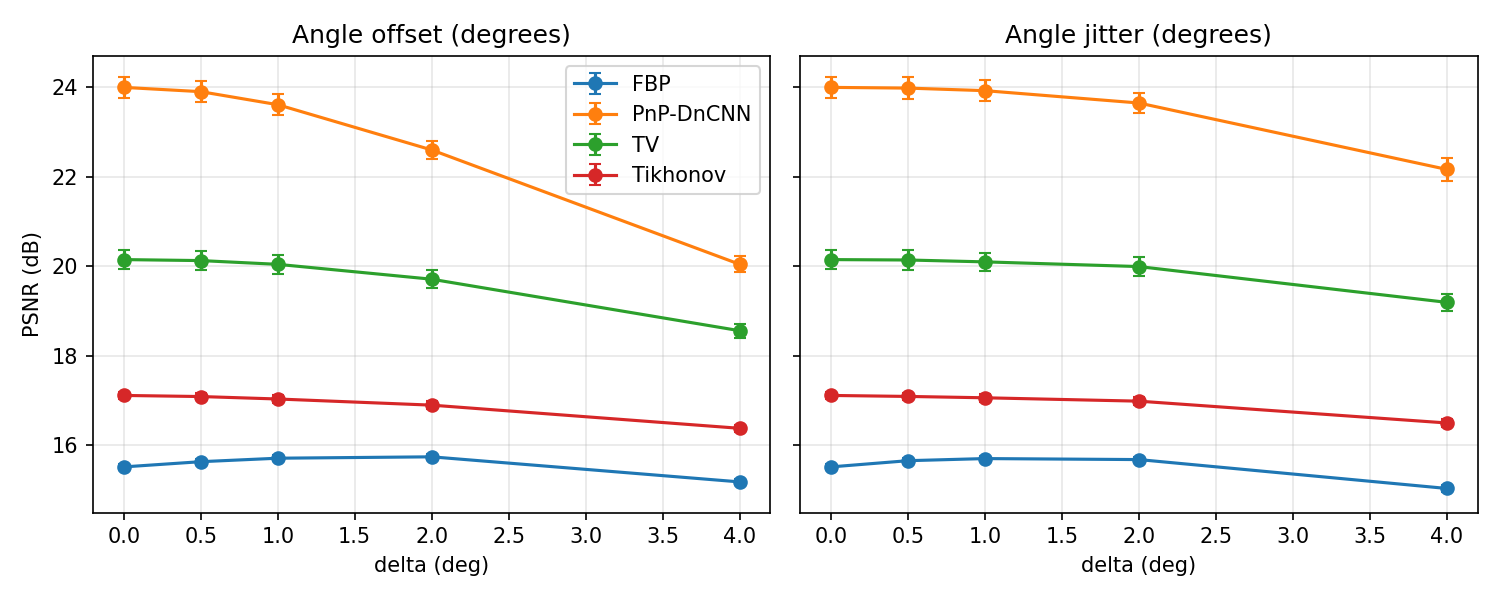
\includegraphics[width=0.95\textwidth]{figures/robust_mismatch.png}
\caption{Test PSNR under forward-model mismatch as a function of the angular perturbation $\delta$ (degrees): constant offset (left) and per-angle jitter with standard deviation $\delta$ (right), TV-ADMM as the TV baseline.
Hyper-parameters are frozen at their nominal values and are not re-tuned. PnP-DnCNN has the highest mean PSNR at every level, and loses more than TV in absolute terms under both perturbations; the offset curve
mainly reflects a rigid rotation of the reconstruction (Table~\ref{tab:e3rot}). Error bars: mean $\pm1.96$ standard errors over 200 test images, which reflect image variability only (a single jitter draw is used).}
\label{fig:robust_mismatch}
\end{figure}

\paragraph{A constant offset is a rotation.}
Data generated at the angles $\theta_j$ are consistent with an operator at the angles $\theta_j+\delta$ if the image is rotated by $\delta$ about the centre. A reconstruction that is perfect up to this rotation is therefore
the best a method can do, yet a pixel-wise metric against the true image penalises it. To separate the two effects we scored each reconstruction against the true digit and against the true digit rotated by $\delta$ (Table~\ref{tab:e3rot};
the opposite direction gives lower agreement). Against the rotated digit PnP keeps its nominal accuracy (24.1--24.2\,dB at all offsets, against 24.0\,dB at $\delta=0$), so the 4.0\,dB loss in Table~\ref{tab:e3} is
registration error, not a loss of reconstruction quality; TV also loses nothing against the rotated digit (it scores 20.4--21.0\,dB against 20.15\,dB nominal; part of this is because the interpolated reference is smoother than the true digit).
The sharper reconstruction has more to lose under a pixel-wise metric: even a perfect reconstruction rotated by $4^\circ$ would score only 22.1\,dB, and PnP's 20.05\,dB is already close to this ceiling.

\begin{table}[htbp]
\centering\small\setlength{\tabcolsep}{6pt}
\caption{Constant offset: PSNR (dB) of the reconstruction against the true digit and against the true digit rotated by $\delta$ (cubic interpolation). The last column is the PSNR of the true digit rotated by $\delta$ against itself, the best score a perfect but rotated reconstruction can reach.
Computed with \texttt{run\_e3\_rotation\_check.py}; the nominal values reproduce the stored E3 results.}\label{tab:e3rot}
\begin{tabular}{lccccc}
\toprule
 & \multicolumn{2}{c}{TV} & \multicolumn{2}{c}{PnP} & \\
\cmidrule(lr){2-3}\cmidrule(lr){4-5}
$\delta$ & vs true & vs rotated & vs true & vs rotated & Ceiling \\
\midrule
$0^\circ$ & 20.15 & 20.15 & 24.00 & 24.00 & $\infty$ \\
$1^\circ$ & 20.04 & 20.36 & 23.62 & 24.14 & 35.9 \\
$2^\circ$ & 19.71 & 20.66 & 22.61 & 24.23 & 29.0 \\
$4^\circ$ & 18.56 & 20.99 & 20.05 & 24.14 & 22.1 \\
\bottomrule
\end{tabular}
\end{table}

\paragraph{Results.}
\emph{(i) Per-angle jitter is the genuine inconsistency.} With a jitter of $4^\circ$ (s.d.) PnP loses $1.8$\,dB and TV $1.0$\,dB; the advantage falls from $+3.86$ to $+2.98$\,dB and PnP stays ahead on 99\% of the images.
\emph{(ii) Constant offset.} In raw PSNR PnP loses $4.0$\,dB against $1.6$\,dB for TV and the advantage falls to $+1.49$\,dB (still positive on 96\% of the images). Table~\ref{tab:e3rot} shows that this is a registration effect, so it
should not be read as evidence that PnP is the less robust method to a rigid geometric error; it is evidence that PSNR penalises a sharp but shifted reconstruction more.
\emph{(iii) What is not shown.} Neither method collapses within the range tested, but both TV-ADMM and the PnP parameters are frozen, so the experiment measures the sensitivity of nominally tuned methods, not what a re-tuned method would achieve.

\paragraph{Caveats.}
(a)~One jitter draw per level and one noise realisation; the intervals describe image variability only. (b)~Only the projection angles are perturbed (no detector offset, scale or beam-hardening errors), at $\sigma=0.05$,
on inverse-crime data. (c)~Frozen hyper-parameters: a mismatch acts like extra noise, so re-tuning might favour a larger $\sigma_d$ for PnP and a larger $\lambda$ for TV; we did not test this. (d)~TV-ADMM is unconstrained; the TV-box control
was not run for E3.


\subsection{E4: Distribution shift}\label{sec:e4}
\paragraph{Setting.}
The denoiser is trained on MNIST digits only. The complete pipeline, with hyper-parameters tuned once on the MNIST validation images at $\sigma=0.05$ and 20 angles (TV-ADMM $\lambda=5.6\times10^{-3}$; PnP $\sigma_d=0.1$, $k=5$) and then frozen, is
applied to 200 Fashion-MNIST test images, 200 EMNIST letters, and a $28\times28$ Shepp--Logan phantom. The phantom is a single image, so its 20 test cases are 20 independent noise draws and its
interval describes noise variability only. Data are generated with the reconstruction operator (inverse crime) with a different noise realisation from E1, so the MNIST row differs slightly from Table~\ref{tab:e1e2}. The labels ``near'' and ``far''
shift are our a priori judgement; no distance between the distributions was computed.

\begin{table}[htbp]
\centering\small\setlength{\tabcolsep}{4pt}
\caption{Test PSNR and SSIM under distribution shift with the pipeline frozen at its MNIST values (one MNIST-trained denoiser, TV-ADMM). Gap $=$ PnP$-$TV PSNR, mean $\pm1.96$ standard errors of the paired difference
(over images; over noise draws for the phantom); ``wins'' is the share of test cases in which PnP has the higher PSNR.}
\label{tab:e4}
\begin{tabular}{lccccccc}
\toprule
 & \multicolumn{3}{c}{PSNR (dB)} & & \multicolumn{2}{c}{SSIM} \\
\cmidrule(lr){2-4}\cmidrule(lr){6-7}
Test set & TV & PnP & gap (wins) & & TV & PnP \\
\midrule
MNIST (in-distribution)       & 20.27 & \textbf{23.97} & $+3.70\pm0.16$ (100\%) & & 0.742 & \textbf{0.944} \\
EMNIST letters (near shift)   & 20.09 & \textbf{22.03} & $+1.94\pm0.18$ (92\%)  & & 0.842 & \textbf{0.938} \\
Fashion-MNIST (far shift)     & \textbf{19.61} & 16.57 & $-3.05\pm0.31$ (11\%) & & 0.680 & 0.675 \\
Shepp--Logan (far shift)      & \textbf{19.19} & 15.03 & $-4.16\pm0.19$ (0\%)  & & \textbf{0.722} & 0.517 \\
\bottomrule
\end{tabular}
\end{table}

\begin{figure}[htbp]
\centering
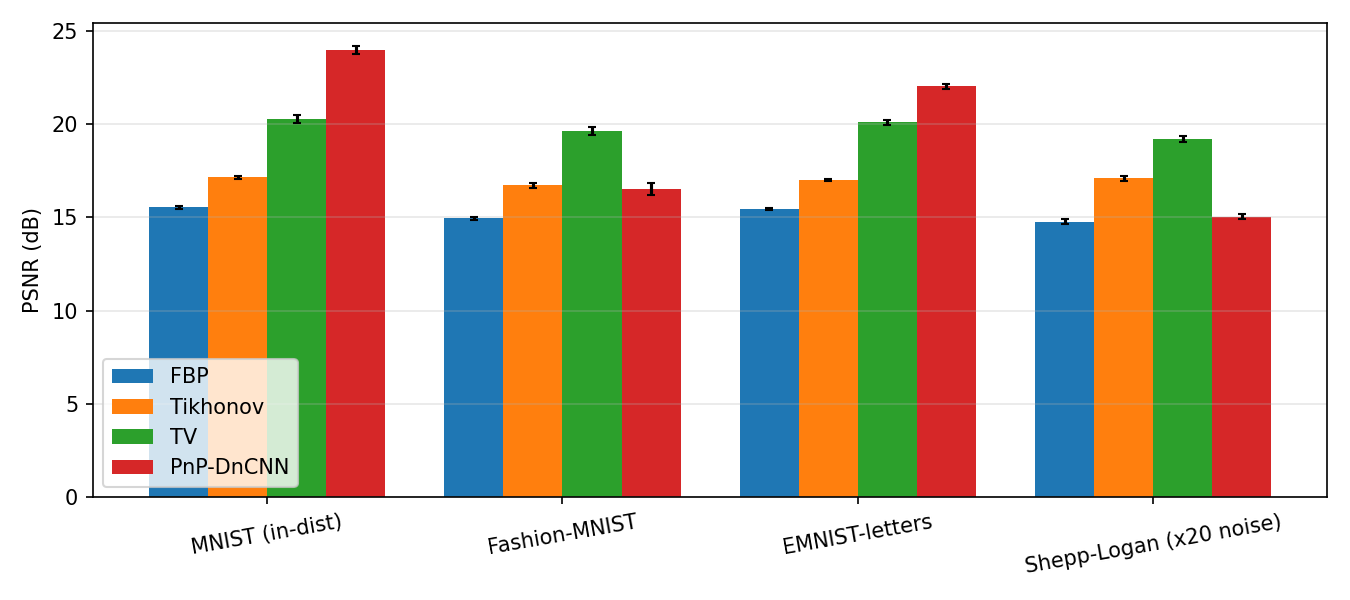
\includegraphics[width=0.8\textwidth]{figures/robust_shift.png}
\caption{Test PSNR under distribution shift for the four methods with the pipeline frozen at its MNIST values. PnP-DnCNN leads on MNIST and on EMNIST letters, which share the stroke-like statistics of digits,
but is below TV on Fashion-MNIST ($-3.0$\,dB) and on the phantom ($-4.2$\,dB). Against Tikhonov it is $0.2$\,dB below on Fashion-MNIST and $2.1$\,dB below on the phantom; against FBP it is $1.6$\,dB above on Fashion-MNIST and only $0.3$\,dB
above on the phantom. Error bars: mean $\pm1.96$ standard errors; for the phantom they describe 20 noise draws of one image, not variation between images.}
\label{fig:robust_shift}
\end{figure}

\begin{table}[htbp]
\centering\small\setlength{\tabcolsep}{4pt}
\caption{Control with a box-constrained TV (TV-box, $0\le x\le1$, 1000 iterations, $\lambda$ tuned on the MNIST validation images). Three independently trained MNIST denoisers (E8), bicubic fine-grid data,
$\sigma=0.05$, 20 angles. Mean test PSNR over the three denoisers and gap $=$ PnP$-$TV, mean $\pm$ s.d.\ over denoisers.}\label{tab:e4box}
\begin{tabular}{lccccc}
\toprule
Test set & TV-ADMM & TV-box & PnP & PnP$-$TV-ADMM & PnP$-$TV-box \\
\midrule
MNIST          & 20.21 & 20.69 & 24.05 & $+3.84\pm0.03$ & $+3.36\pm0.03$ \\
EMNIST letters & 20.28 & 20.35 & 22.07 & $+1.79\pm0.09$ & $+1.72\pm0.09$ \\
Fashion-MNIST  & 19.42 & 19.45 & 16.32 & $-3.10\pm0.30$ & $-3.13\pm0.30$ \\
Shepp--Logan   & 19.28 & 19.50 & 14.96 & $-4.33\pm0.12$ & $-4.55\pm0.12$ \\
\bottomrule
\end{tabular}
\end{table}

\begin{figure}[htbp]
\centering
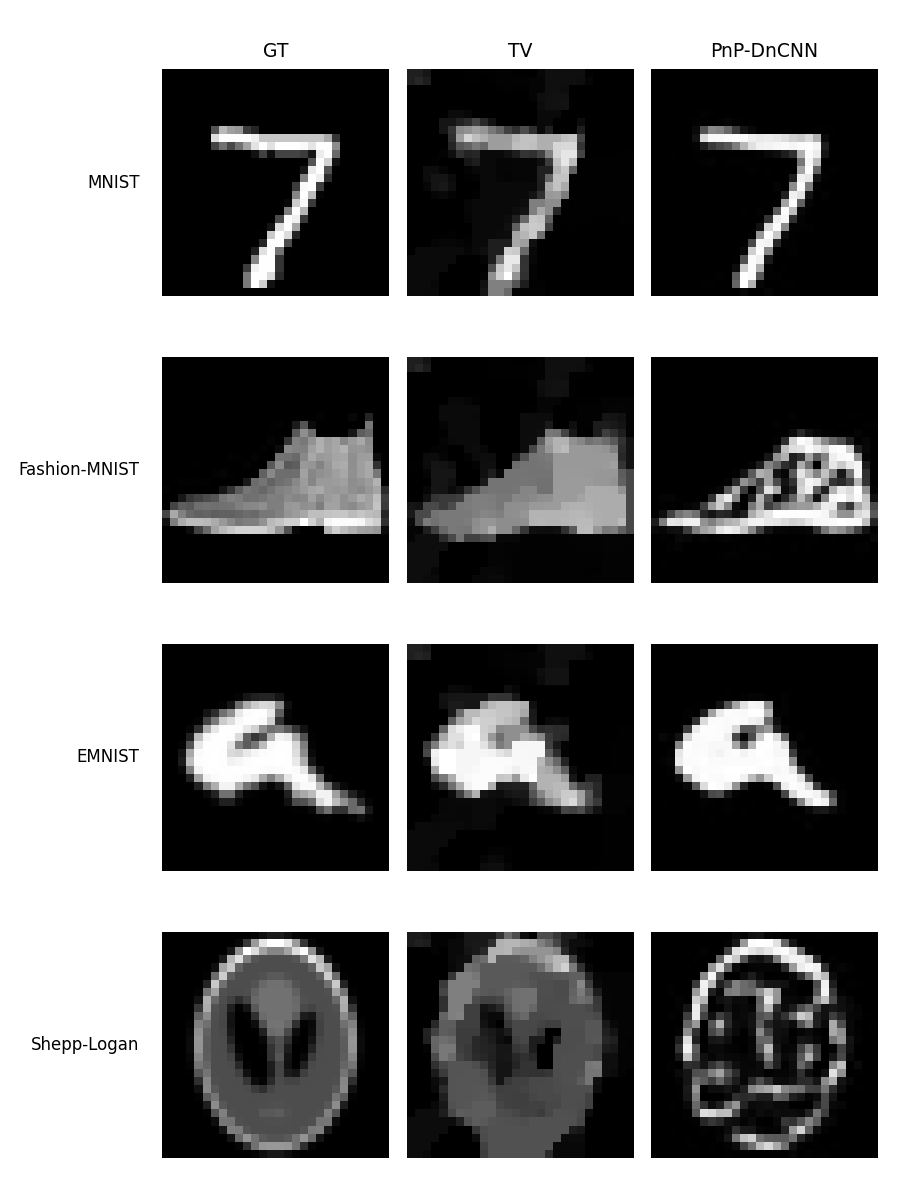
\includegraphics[width=0.6\textwidth]{figures/fig_shift_grid.png}
\caption{Reconstructions at $\sigma=0.05$, 20 angles, with the frozen pipeline: the first test image of each set (no selection), one noise draw, TV-ADMM and the single MNIST-trained PnP denoiser of Table~\ref{tab:e4}.
On Fashion-MNIST and the phantom the PnP output contains spotted or stroke-like fragments that are absent from the ground truth; the TV output is blurred and blocky but does not introduce such structure. A TV-box column and PSNR values are not shown.}
\label{fig:shift}
\end{figure}

\paragraph{Results.}
\emph{(i) The advantage does not transfer to far-shifted images.} On EMNIST letters PnP keeps about half of its in-distribution advantage ($+1.9$ against $+3.7$\,dB). On Fashion-MNIST and the phantom it is below TV, in 89\% and 100\% of the test cases respectively (Table~\ref{tab:e4}).
The reversal is not an artefact of the unconstrained TV: with a box-constrained TV the gaps are $-3.13$ and $-4.55$\,dB, slightly larger than against TV-ADMM, because the box constraint helps TV on the phantom by $0.2$\,dB and on Fashion-MNIST by $0.03$\,dB (Table~\ref{tab:e4box}). The in-distribution advantage, in contrast,
loses $0.5$\,dB to the box constraint ($+3.84\to+3.36$\,dB).
\emph{(ii) Variability.} Across three independently trained MNIST denoisers the Fashion-MNIST gap has a standard deviation of $0.30$\,dB and the phantom gap $0.12$\,dB (Table~\ref{tab:e4box}); the single denoiser of Table~\ref{tab:e4} gives similar values ($-3.05$ and $-4.16$\,dB, on a different data model) and the sign never changes.
\emph{(iii) PSNR and SSIM disagree on Fashion-MNIST.} PnP is $3.1$\,dB below TV in PSNR but equal in SSIM ($0.675$ against $0.680$), while on the phantom both are clearly lower ($0.517$ against $0.722$). We did not examine why; a plausible reading is that the PnP error on Fashion-MNIST is
mainly in smooth intensity levels that SSIM tolerates, which is untested.
\emph{(iv) Structure rather than blur.} In Figure~\ref{fig:shift}, TV fails by blurring, whereas PnP adds structure not present in the image. This is a qualitative observation on one image per set. It is quantified with inserted lesions in
Section~\ref{sec:lesion-results}: for the MNIST-trained prior on Fashion-MNIST, PnP produces $0.38$ false lesions per lesion-absent image, against $0.14$ for TV-box and $0.05$ for TV-ADMM (means over three denoisers and eight lesion types).
The converse experiment, in which a prior trained on Fashion-MNIST is tested on Fashion-MNIST, is in Section~\ref{sec:seeds-results}.

\paragraph{Caveats.}
(a)~The pipeline is frozen at MNIST-tuned values. The deficit therefore combines a mismatched prior with mismatched hyper-parameters, and we did not test whether re-tuning $\sigma_d$ and $k$ on the target set would reduce it; the matched-prior control of E8 changes the prior and the tuning set together.
(b)~The phantom is one image, so the ``far shift'' evidence on it is one object; Fashion-MNIST supplies the only far-shift evidence over many images. (c)~Table~\ref{tab:e4} uses inverse-crime data and Table~\ref{tab:e4box} crime-free data; the conclusions agree, but the numbers are not interchangeable.
(d)~Only three datasets are used, so no claim about how the deficit scales with the distance between distributions can be made.


\subsection{E5: Why PnP selects few iterations}\label{sec:e5}
\paragraph{Setting.}
Validation tuning selects few iterations: $k=5$ at $\sigma\le0.05$ with 20 or 90 angles, $10$ at $\sigma=0.1$ or 40 angles, $25$ at $\sigma=0.2$ or 10 angles, and $100$ at 5 angles (E1--E2). To see what happens beyond the selected $k$ we
ran the tuned pipeline ($\sigma=0.05$, 20 angles, inverse-crime data, 200 test digits) with $\sigma_d\in\{0.02,0.05,0.1,0.2\}$ and recorded the iterate at $k\in\{1,2,5,10,25,50,100,200,400\}$ (so the location of a peak is resolved only to this grid).
For each iterate we computed the PSNR, the data residual $\lVert Ax_k-y\rVert$ relative to the noise norm $\sigma\sqrt{m}$, and the squared error in bands of the singular values $s_i$ of $A$ relative to the largest, $s_i/s_1$ (the decomposition of Section~\ref{sec:subspace}).
The tuned setting is $(\sigma_d,k)=(0.1,5)$.

\begin{figure}[htbp]
\centering
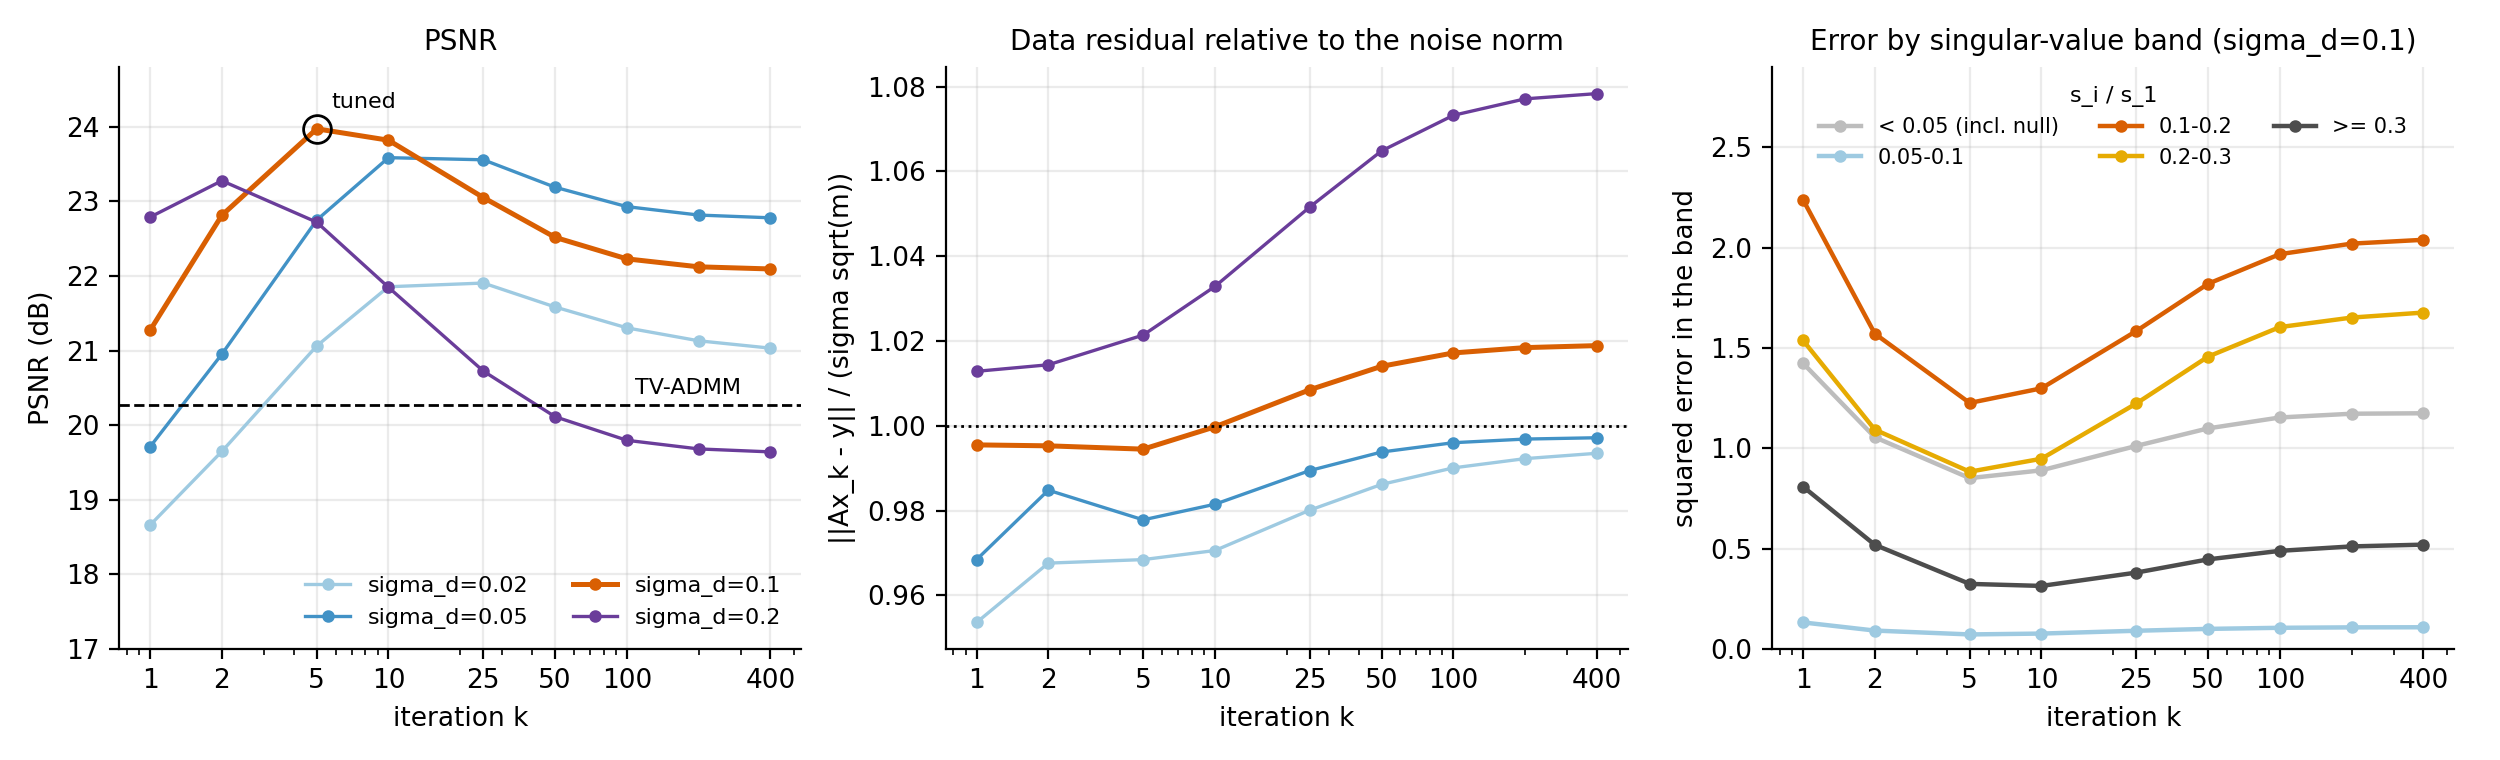
\includegraphics[width=\textwidth]{figures/fig_e5_iterations.png}
\caption{PnP iterates on 200 MNIST test digits ($\sigma=0.05$, 20 angles). Left: PSNR against the iteration count $k$ for four denoiser strengths; the circle marks the tuned setting and the dashed line is TV-ADMM.
Middle: data residual relative to the expected noise norm $\sigma\sqrt{m}$. Right: squared error in bands of $s_i/s_1$ for $\sigma_d=0.1$ (the bands contain 319, 46, 253, 129 and 37 of the 784 directions, in the order of the legend). Every point is one run with one noise draw.}
\label{fig:convergence}
\end{figure}

\paragraph{Results.}
\emph{(i) Early stopping is necessary at every $\sigma_d$ tested.} For $\sigma_d=0.1$ the PSNR peaks at $k=5$ ($23.97$\,dB) and falls to $22.09$\,dB at $k=400$ (Figure~\ref{fig:convergence}, left). The decay is stronger for larger $\sigma_d$ ($\sigma_d=0.2$: $23.28$\,dB at $k=2$ to $19.64$\,dB at $k=400$, below TV's $20.27$\,dB) and weaker for smaller ones. Among the four $\sigma_d$ the best converged
setting is $\sigma_d=0.05$ at $22.78$\,dB: $1.2$\,dB below the early-stopped optimum, but still $2.5$\,dB above TV. Early stopping is therefore worth about 1\,dB here and is not what makes PnP better than TV in distribution.

\emph{(ii) The data residual stays at the noise level.} For $\sigma_d=0.1$ the ratio $\lVert Ax_k-y\rVert/(\sigma\sqrt m)$ moves from $0.994$ at the selected iterate to $1.019$ at $k=400$ (at most $1.08$ for $\sigma_d=0.2$) (Figure~\ref{fig:convergence}, middle). The iterates are
data-consistent to within a few percent of the noise level at every $k$, and the residual changes by 2.5\% between the best and the converged iterate; a discrepancy-principle stopping rule could not pick $k=5$ from it. The earlier reading that the denoiser's prior increasingly dominates the data term
is not supported by these data: the iteration converges, and it converges to a point that fits the data as well as the early iterates do but has a larger error.

\emph{(iii) Where the error grows.} Between $k=5$ and $k=400$ ($\sigma_d=0.1$) the squared error rises from $3.36$ to $5.52$. Of this increase of $2.16$, $74\%$ lies in the directions with $0.1\le s_i/s_1<0.3$ (382 of 784 directions), $17\%$ in the directions below $0.1$ (including the exact null space), $10\%$ in $0.3\le s_i/s_1<0.5$, and none in the directions with $s_i/s_1\ge0.5$, where the error does not
grow (Figure~\ref{fig:convergence}, right). The gradient step contracts the error in direction $i$ by $(1-(s_i/s_1)^2)^k$ (Section~\ref{sec:nullspace-results}), i.e.\ by $0.82$ for $s_i/s_1=0.2$ after 5 iterations, $0.36$ after 25 and $0.02$ after 100. These directions therefore become determined by the data
at about the iterations where the PSNR declines (10 to 100), which is what classical semi-convergence of iterative regularisation predicts: further iterations fit the noise in poorly determined directions. This is consistent with the data, not a test of the mechanism. In particular, the tuned $k$ is also $5$ at $\sigma=0$ (E1), so noise fitting cannot be the only cause; we did not record the iteration curve on noise-free data.

\begin{table}[htbp]
\centering\small\setlength{\tabcolsep}{4pt}
\caption{PSNR (dB) of PnP at the tuned setting ($\sigma_d=0.1$, $k=5$), run to $k=400$ with the same $\sigma_d$, and at the best $(\sigma_d,k)$ over the stored grid ($\sigma_d\in\{0.02,\dots,0.2\}$, $k\in\{1,\dots,400\}$), selected on the test images themselves and therefore optimistic. Same frozen pipeline, noise draws and TV-ADMM as E4; the phantom is one image with 20 noise draws.}\label{tab:e5}
\begin{tabular}{lccccc}
\toprule
Test set & TV-ADMM & PnP $k=5$ & PnP $k=400$ & best $(\sigma_d,k)$ & FBP \\
\midrule
MNIST (in-distribution) & 20.27 & 23.97 & 22.09 & 23.97 \,(0.1, 5) & 15.53 \\
EMNIST letters          & 20.09 & 22.03 & 20.11 & 22.03 \,(0.1, 5) & 15.47 \\
Fashion-MNIST           & 19.61 & 16.57 & 13.80 & 17.86 \,(0.2, 1) & 14.94 \\
Shepp--Logan            & 19.19 & 15.03 & 12.40 & 16.36 \,(0.1, 1) & 14.77 \\
\bottomrule
\end{tabular}
\end{table}

\emph{(iv) Under shift, stopping early limits the damage but cannot remove it.} On the two shifted sets the PSNR is highest at $k=1$, and run to convergence PnP is $5.8$\,dB (Fashion-MNIST) and $6.8$\,dB (phantom) below TV and below FBP (Table~\ref{tab:e5}). Even the best setting of the grid stays $1.8$ and $2.8$\,dB below TV.
The in-distribution benefit of early stopping and the shift deficit may share a cause, namely that more iterations let the prior shape the result further, but this is an interpretation and was not tested.

\paragraph{Caveats.}
(a)~Single noise draw, one denoiser, four $\sigma_d$ values, and checkpoints rather than every iteration (the peak lies between $k=5$ and $10$; a per-iteration curve on 50 images in an earlier version of this figure peaked at about $k=5$ for $\sigma_d=0.1$). (b)~The band decomposition is reported for $\sigma_d=0.1$ only. (c)~The ``best'' setting in Table~\ref{tab:e5} is chosen on test data.
(d)~Inverse-crime data; Section~\ref{sec:nullspace-results} repeats the analysis on crime-free data.


\subsection{E6: Sensitivity to the inverse crime}\label{sec:crime-results}
\paragraph{Setting.}
E1--E5 generate the data with the reconstruction matrix $A$. Here the measurements are instead simulated on a five-times finer grid with three object resamplings (nearest, bicubic, bilinear; Section~\ref{sec:crimefree}), and compared with the inverse-crime data. The mean model error
$\lVert\mathcal{S}(x)-Ax\rVert_2$ is $0$, $0.03$, $0.09$ and $0.10$ for the inverse crime, nearest, bicubic and bilinear data (20 angles); for comparison, the noise norm $\sigma\sqrt m$ is $0.28$, $1.41$, $2.83$ and $5.66$ for $\sigma=0.01,0.05,0.1,0.2$.
With crime-free data the case $\sigma=0$ is therefore not noise-free: the only error in the measurements is the model error. Hyper-parameters of all methods are re-tuned for each data model. The PnP$-$TV gaps below are against TV-ADMM unless stated; there is one noise draw and one denoiser per cell.

\begin{table}[htbp]
\centering\small\setlength{\tabcolsep}{5pt}
\caption{PnP$-$TV PSNR gap (dB), 20 angles, 200 test digits, for four data models. TV is TV-ADMM except in the last two rows, which use the box-constrained TV-box (E2b control, only run for the inverse-crime and bicubic data).
$\dagger$: the TV-box optimum lies below the initial $\lambda$ grid (Table~\ref{tab:e1e2}).}\label{tab:crime}
\begin{tabular}{lccccccc}
\toprule
Data model & Model error & $\sigma=0$ & $0.01$ & $0.05$ & $0.1$ & $0.2$\\
\midrule
Same operator (inverse crime)            & 0     & $-6.43$ & $+0.07$ & $+3.86$ & $+3.01$ & $+1.03$\\
Fine grid, nearest                       & 0.03  & $-5.86$ & $+0.16$ & $+3.86$ & $+3.01$ & $+1.02$\\
Fine grid, bicubic (default)             & 0.09  & $-3.29$ & $+1.02$ & $+4.02$ & $+3.10$ & $+1.08$\\
Fine grid, bilinear                      & 0.10  & $-0.97$ & $+1.76$ & $+3.94$ & $+2.87$ & $+0.85$\\
\midrule
Inverse crime, vs TV-box                 & 0     & $-12.93^\dagger$ & $-0.75$ & $+3.33$ & $+2.65$ & $+0.65$\\
Bicubic, vs TV-box                       & 0.09  & $-5.13$ & $+0.35$ & $+3.48$ & $+2.73$ & $+0.69$\\
\bottomrule
\end{tabular}
\end{table}

\begin{table}[htbp]
\centering\small\setlength{\tabcolsep}{5pt}
\caption{PnP$-$TV-ADMM PSNR gap (dB) in the angle sweep ($\sigma=0.05$) for the four data models. The mean model error of the bicubic data is $0.05$, $0.07$, $0.09$, $0.12$, $0.17$ at $5,10,20,40,90$ angles.}\label{tab:crimeang}
\begin{tabular}{lccccc}
\toprule
Data model & 5 & 10 & 20 & 40 & 90 \\
\midrule
Same operator (inverse crime) & $+2.13$ & $+3.03$ & $+3.86$ & $+3.83$ & $+3.04$ \\
Fine grid, nearest            & $+2.19$ & $+3.04$ & $+3.86$ & $+3.84$ & $+3.06$ \\
Fine grid, bicubic (default)  & $+2.36$ & $+3.29$ & $+4.02$ & $+3.97$ & $+3.24$ \\
Fine grid, bilinear           & $+2.17$ & $+3.23$ & $+3.94$ & $+4.04$ & $+3.57$ \\
\bottomrule
\end{tabular}
\end{table}

\begin{table}[htbp]
\centering\small\setlength{\tabcolsep}{5pt}
\caption{As Table~\ref{tab:e1e2}, with measurements simulated on the finer grid (bicubic, $f=5$); mean test PSNR (dB) over 200 digits. The last column is the PnP$-$TV-ADMM gap.
Intervals and TV-box results are in Table~\ref{tab:e1e2gap}.}\label{tab:table1fine}
\begin{tabular}{lccccc}
\toprule
Condition & FBP & Tikhonov & TV-ADMM & PnP-DnCNN & PnP$-$TV\\
\midrule
$\sigma=0$, 20 angles    & 24.3 & 27.4 & 33.2 & 29.9 & $-3.29$\\
$\sigma=0.01$, 20 angles & 23.2 & 23.9 & 28.4 & 29.4 & $+1.02$\\
$\sigma=0.05$, 20 angles & 15.5 & 17.1 & 20.1 & 24.1 & $+4.02$\\
$\sigma=0.1$, 20 angles  & 10.4 & 14.7 & 16.8 & 19.9 & $+3.10$\\
$\sigma=0.2$, 20 angles  &  6.6 & 12.9 & 14.3 & 15.3 & $+1.08$\\
5 angles, $\sigma=0.05$  &  9.1 & 14.1 & 15.5 & 17.8 & $+2.36$\\
10 angles, $\sigma=0.05$ & 12.1 & 15.9 & 18.2 & 21.5 & $+3.29$\\
40 angles, $\sigma=0.05$ & 18.1 & 18.2 & 21.8 & 25.8 & $+3.97$\\
90 angles, $\sigma=0.05$ & 20.7 & 20.0 & 24.1 & 27.3 & $+3.24$\\
\bottomrule
\end{tabular}
\end{table}

\begin{figure}[htbp]
\centering
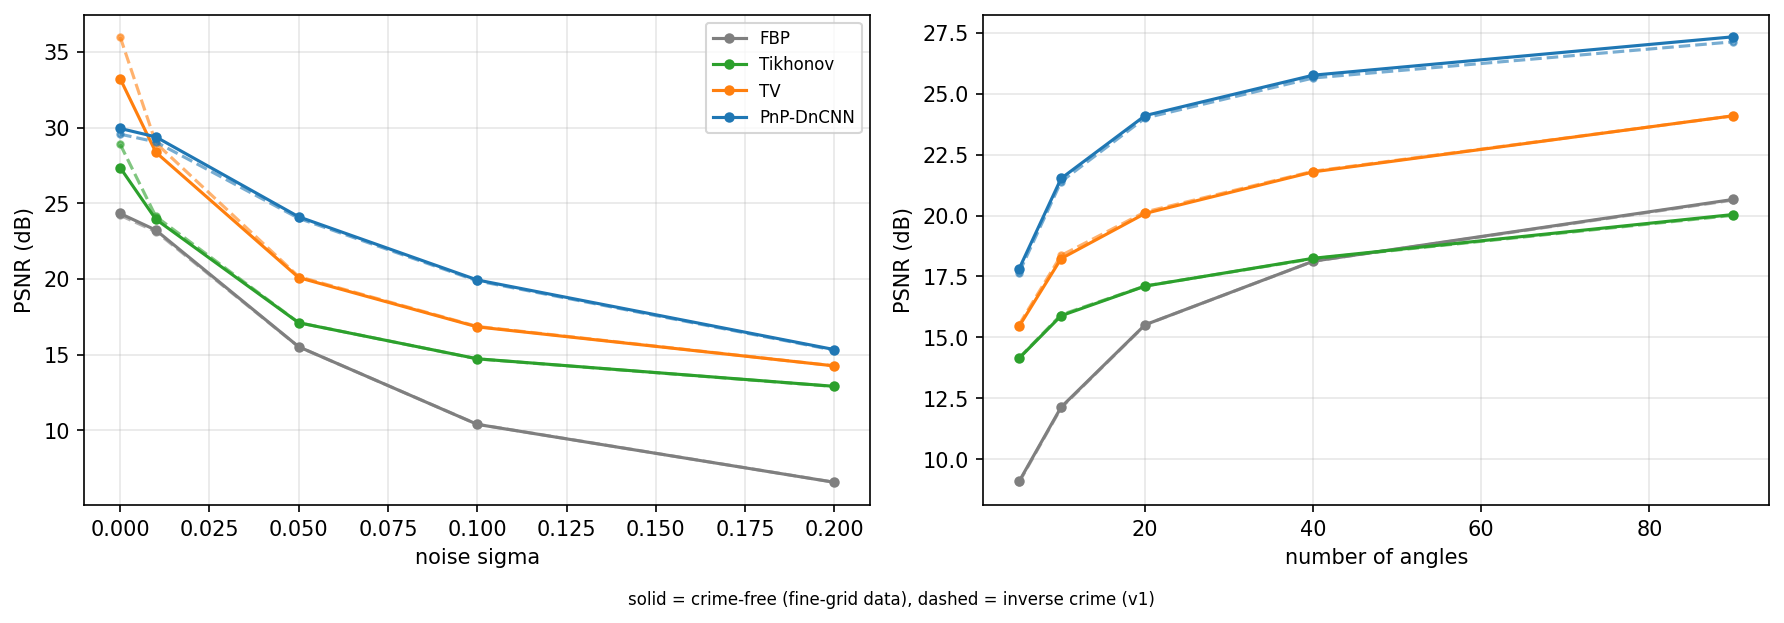
\includegraphics[width=\linewidth]{figures/crime_comparison.png}
\caption{PSNR versus noise level (left) and number of angles (right) for data simulated on the bicubic finer grid (solid) and with the inverse crime (dashed), TV-ADMM as the TV baseline. The curves nearly coincide for $\sigma\ge0.05$ and separate at $\sigma\le0.01$, where TV loses $2.8$\,dB at $\sigma=0$ ($36.0\to33.2$\,dB) while PnP gains $0.3$\,dB.}\label{fig:crime}
\end{figure}

\paragraph{Results.}
\emph{(i) The conclusions at $\sigma\ge0.05$ do not depend on the data model.} The model error is at most 7\% of the noise norm there, and the PnP$-$TV-ADMM gap differs between the inverse-crime and the bicubic data by at most $0.16$\,dB in the noise sweep (Table~\ref{tab:crime}) and $0.26$\,dB in the angle sweep (Table~\ref{tab:crimeang}); between the inverse-crime and the bilinear data it differs by up to $0.53$\,dB (90 angles).
Against TV-box the gap is $0.4$ to $0.5$\,dB smaller than against TV-ADMM on both data models but keeps its sign (Table~\ref{tab:crime}, last rows).

\emph{(ii) The low-noise end depends on the data model, and also on the TV solver.} At $\sigma=0$ TV is ahead of PnP in every variant, by $6.4$\,dB (inverse crime), $5.9$ (nearest), $3.3$ (bicubic) and $1.0$\,dB (bilinear); against TV-box the lead is larger ($12.9$\,dB, with the TV-box optimum below the $\lambda$ grid, and $5.1$\,dB). At $\sigma=0.01$ the PnP lead against TV-ADMM ranges from $+0.07$ to $+1.76$\,dB across the four data models, and against TV-box it is $-0.75$\,dB (inverse crime) or $+0.35$\,dB (bicubic).
The ranking at $\sigma\le0.01$ is therefore not a single number: it changes with the data model by up to $5.5$\,dB at $\sigma=0$ and changes sign with the choice of TV solver and data model at $\sigma=0.01$. We make no claim about PnP versus TV at $\sigma\le0.01$ from the digit experiments. A possible reading is that TV, tuned for $\sigma\approx0$, fits the data almost exactly and is penalised when the data contain model error, whereas PnP is not; we did not test this.

\emph{(iii) Out-of-distribution deficits persist.} With the pipeline of E4 the PnP$-$TV-ADMM gap is $-3.05$ (inverse crime), $-3.04$, $-2.82$ and $-3.88$\,dB on Fashion-MNIST, and $-4.16$, $-4.16$, $-4.21$ and $-5.37$\,dB on the phantom, for the four data models in the order of Table~\ref{tab:crime}; the in-distribution EMNIST advantage stays between $+1.8$ and $+1.9$\,dB. The deficits are largest for the bilinear data, whose object is the smoothest.

\emph{(iv) The default data model.} We use the bicubic data as the default crime-free setting for the later experiments. The choice was made after seeing all four variants, because its low-noise results lie between those of the nearest and the bilinear data; it is a convention, not a derived optimum, and the results at $\sigma\le0.01$ should be read as the band spanned by the variants.

\paragraph{Caveats.}
(a)~One noise draw and one denoiser per cell; hyper-parameters are re-tuned for each data model, so part of the differences between rows is tuning. (b)~The model error is a deterministic resampling difference, not the unknown mismatch of a real scanner; the real-data setting is addressed in Stage~3 (Section~\ref{sec:e14}).
(c)~TV-box was run for two of the four data models; the other experiments of this section use TV-ADMM.


\subsection{E7: Error decomposition along the singular vectors}\label{sec:nullspace-results}
\paragraph{Setting.}
We apply the decomposition of Section~\ref{sec:subspace} to the shift setting of E4 on crime-free (bicubic) data: the MNIST-trained denoiser with the pipeline tuned on MNIST and frozen, $\sigma=0.05$, 20 angles, 200 test images per set (the phantom: 20 noise draws of one image).
The weakly determined subspace is $W_{0.05}$ ($s_i<0.05\,s_1$, $\dim W_{0.05}=319$ of 784, containing the 79-dimensional exact null space); $W^\perp$ is its complement. We report the squared error in each part as the ratio PnP/TV-ADMM (below 1: PnP has less error),
with the injection $\iota$ and alignment $c$ statistics. Paired Wilcoxon tests on the per-image errors give $p<10^{-10}$ for every ratio of the three 200-image sets in Table~\ref{tab:nullspace}; for the phantom, with 20 noise draws, $p=1.9\times10^{-6}$ is the smallest value attainable.

\begin{table}[htbp]
\centering\small\setlength{\tabcolsep}{4pt}
\caption{Error decomposition at $\sigma=0.05$, 20 angles, bicubic fine-grid data, $W_{0.05}$ ($\dim=319$).
Ratios are PnP/TV-ADMM (below 1: PnP has less error); $\iota$ is the injection and $c$ the alignment statistic of
Section~\ref{sec:subspace}.}\label{tab:nullspace}
\begin{tabular}{lccccccc}
\toprule
 & \multicolumn{3}{c}{error ratio PnP/TV} & \multicolumn{2}{c}{$\iota$} & \multicolumn{2}{c}{$c$}\\
\cmidrule(lr){2-4}\cmidrule(lr){5-6}\cmidrule(lr){7-8}
Test set & in $W$ & in $W^\perp$ & total & TV & PnP & TV & PnP\\
\midrule
MNIST (in-dist.)  & 0.48 & 0.40 & 0.42 & 0.58 & 0.76 & 0.45 & 0.76\\
EMNIST letters    & 0.70 & 0.64 & 0.65 & 1.22 & 1.55 & 0.43 & 0.67\\
Fashion-MNIST     & 1.27 & 2.32 & 2.05 & 0.29 & 0.80 & 0.36 & 0.37\\
Shepp--Logan      & 2.59 & 2.64 & 2.63 & 0.44 & 3.27 & 0.09 & 0.23\\
\bottomrule
\end{tabular}
\end{table}

\begin{table}[htbp]
\centering\small\setlength{\tabcolsep}{4pt}
\caption{Sensitivity of Table~\ref{tab:nullspace} to the subspace: the exact null space ($\dim=79$), $W_{0.05}$ (319) and $W_{0.10}$ (365). Error ratio PnP/TV in the subspace and PnP injection $\iota$.}\label{tab:nullspace-tau}
\begin{tabular}{lcccccc}
\toprule
 & \multicolumn{2}{c}{exact null} & \multicolumn{2}{c}{$W_{0.05}$} & \multicolumn{2}{c}{$W_{0.10}$}\\
\cmidrule(lr){2-3}\cmidrule(lr){4-5}\cmidrule(lr){6-7}
Test set & ratio & $\iota$ & ratio & $\iota$ & ratio & $\iota$\\
\midrule
MNIST (in-dist.) & 0.49 & 0.72 & 0.48 & 0.76 & 0.47 & 0.76\\
EMNIST letters   & 0.68 & 1.56 & 0.70 & 1.55 & 0.70 & 1.56\\
Fashion-MNIST    & 1.21 & 0.70 & 1.27 & 0.80 & 1.27 & 0.83\\
Shepp--Logan     & 2.64 & 3.68 & 2.59 & 3.27 & 2.21 & 2.74\\
\bottomrule
\end{tabular}
\end{table}

\begin{figure}[htbp]
\centering
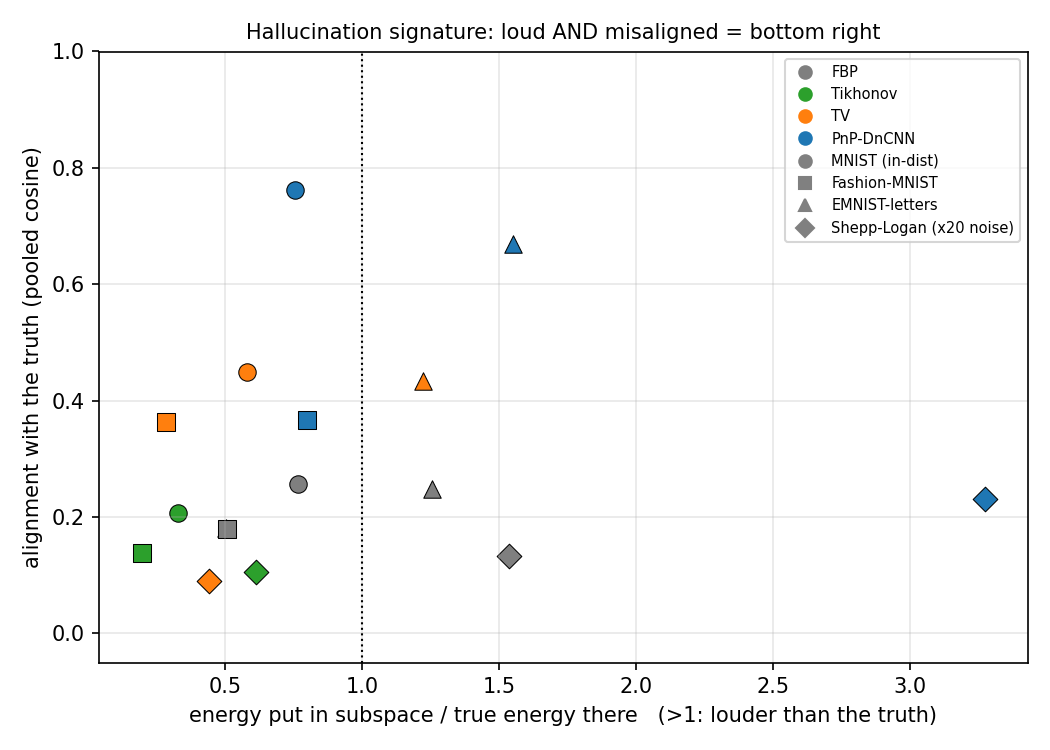
\includegraphics[width=0.75\linewidth]{figures/nullspace_signature_fine5c.png}
\caption{Injection (horizontal axis: energy placed in $W_{0.05}$ divided by the true energy there) against alignment (vertical axis: pooled cosine with the truth in $W_{0.05}$) for each method and test set (bicubic fine-grid data).
Points to the right of the dotted line place more energy in $W_{0.05}$ than the true images contain; low alignment means that this energy does not point in the true direction. Only PnP-DnCNN on the phantom is both loud and poorly aligned.}\label{fig:signature}
\end{figure}

\begin{table}[htbp]
\centering\small\setlength{\tabcolsep}{4pt}
\caption{Total error energy ratio PnP/TV-ADMM as a function of the iteration count, with $\sigma_d=0.1$ and the same frozen pipeline: at the tuned $k=5$, at the best $k$ of the grid $\{1,2,5,10,25,50,100,200,400\}$ (selected on the test images, hence optimistic, with the selected $k$ in brackets) and at $k=400$.
Left: data with the inverse crime ($\sigma_d$ grid of E5); right: bilinear fine-grid data.}\label{tab:nullspace-k}
\begin{tabular}{lcccccc}
\toprule
 & \multicolumn{3}{c}{Inverse crime} & \multicolumn{3}{c}{Bilinear fine grid}\\
\cmidrule(lr){2-4}\cmidrule(lr){5-7}
Test set & $k=5$ & best $k$ & $k=400$ & $k=5$ & best $k$ & $k=400$\\
\midrule
MNIST (in-dist.) & 0.43 & 0.43 (5) & 0.71 & 0.43 & 0.42 (5) & 0.65\\
EMNIST letters   & 0.64 & 0.64 (5) & 1.01 & 0.66 & 0.62 (5) & 0.93\\
Fashion-MNIST    & 2.16 & 1.56 (2) & 4.13 & 2.65 & 1.47 (2) & 3.71\\
Shepp--Logan     & 2.60 & 1.92 (1) & 4.77 & 3.44 & 1.89 (1) & 4.58\\
\bottomrule
\end{tabular}
\end{table}

\paragraph{Results.}
\emph{(i) In distribution the advantage is not confined to the unobserved directions.} On MNIST PnP has $0.48$ times TV's error in $W_{0.05}$ and $0.40$ times in its complement, and its content in $W_{0.05}$ is better aligned with the truth ($c=0.76$ against $0.45$). The same holds for EMNIST letters ($0.70$ and $0.64$).
Since a gradient step never changes the null-space component, the null-space error reduction (ratio $0.49$ in the exact null space, Table~\ref{tab:nullspace-tau}) is entirely due to the denoiser.

\emph{(ii) Under shift the excess error is mostly in the observed directions.} On Fashion-MNIST the ratios are $1.27$ in $W_{0.05}$ and $2.32$ in $W^\perp$, on the phantom $2.59$ and $2.64$. Because $W^\perp$ contains most of the error energy, $93\%$ (Fashion-MNIST) and $89\%$ (phantom) of PnP's excess error over TV lies outside $W_{0.05}$.
The failure under shift is therefore not confined to the weakly determined subspace. These conclusions hold for the exact null space and for $W_{0.10}$ (Table~\ref{tab:nullspace-tau}); the phantom injection falls from $3.7$ to $2.7$ with the threshold but stays above 1 throughout.

\emph{(iii) The injection--alignment signature separates the two shifted sets.} On the phantom PnP places $3.3$ times the true energy in $W_{0.05}$ (TV: $0.44$) with an alignment of only $0.23$ (TV: $0.09$; Figure~\ref{fig:signature}), whereas on MNIST its injection of $0.76$ comes with an alignment of $0.76$.
On Fashion-MNIST the injection is $0.80$ with alignment $0.37$, no different from TV: PnP's excess error there lies in $W^\perp$ and is not visible in this statistic. The statistic does not by itself distinguish prior-driven structure from amplified noise (Section~\ref{sec:subspace});
the evidence that the phantom injection is driven by the prior is the comparison of E8, where denoisers trained on Fashion-MNIST give an injection of $0.30$--$0.35$ against $2.8$--$3.4$ for MNIST-trained ones, with identical noise and solver.

\emph{(iv) Iterations.} The gradient step, ignoring the denoiser, contracts the error in direction $i$ after $k$ iterations by $(1-(s_i/s_1)^2)^k$: at $k=5$ a direction with $s_i=0.1\,s_1$ retains $95\%$ of its initial error, $s_i=0.3\,s_1$ $62\%$ and $s_i=0.5\,s_1$ $24\%$, so the tuned iteration leaves a large share of directions to the denoiser.
On the shifted sets no setting recovers TV's accuracy: even the best $k$ at $\sigma_d=0.1$ has $1.5$--$1.9$ times TV's error, and the error grows with $k$ to $3.7$--$4.8$ times at $k=400$ (Table~\ref{tab:nullspace-k}). In distribution the converged iterate ($k=400$) remains better than TV on MNIST ($0.65$--$0.71$) and is on par with it on EMNIST letters ($0.93$--$1.01$). Section~\ref{sec:e5} shows where along the singular-value axis the error grows with $k$.

\paragraph{Caveats.}
(a)~All statistics are for one denoiser, one noise draw per image and one data model per table; the phantom is a single object. (b)~The threshold $\tau=0.05$ is a convention (there is no gap in the singular values); Table~\ref{tab:nullspace-tau} shows that the conclusions do not depend on it, but the numbers do. (c)~The error ratio is a ratio of means of squared errors; the Wilcoxon tests are paired over images.
(d)~Table~\ref{tab:nullspace-k} uses two data models other than the one of Table~\ref{tab:nullspace} (no bicubic iteration sweep was run), and the best $k$ is selected on the test images.


\subsection{E8: Denoiser seeds and matched-prior control}\label{sec:seeds-results}
This experiment asks whether the distribution-shift results of E4 depend on the particular denoiser that was trained, and
whether the reversal on Fashion-MNIST is caused by the prior itself or by something else in the pipeline. Table~\ref{tab:seeds}
repeats the shift experiment with three independently trained denoisers per configuration (bicubic data, $\sigma=0.05$, 20 angles).
Three families are used: \emph{m03} (trained on MNIST, $\sigma_{\max}=0.3$, seeds 0--2), \emph{m05} (MNIST, $\sigma_{\max}=0.5$)
and \emph{f03} (Fashion-MNIST, $\sigma_{\max}=0.3$). Within each run all methods are tuned on the validation split of the
family's own training distribution, then frozen; the noise-level grid for $\sigma_d$ was extended to $0.5$.

\paragraph{Seed variation.} Seed-to-seed variation of the gap is at most $0.3$\,dB (standard deviation over three seeds), an order of
magnitude below the effects of interest. On Fashion-MNIST the MNIST-trained prior is $3.10\pm0.30$\,dB below TV-ADMM (range
$-3.43$ to $-2.83$) and on the phantom $4.33\pm0.12$\,dB below. Training with $\sigma_{\max}=0.5$ instead of $0.3$ leaves
these results essentially unchanged (Fashion-MNIST $-3.12\pm0.31$, phantom $-3.94\pm0.02$\,dB). With three seeds the standard
deviations are themselves imprecise, so we read them as an indication of scale rather than as interval estimates.
The sign of every shift effect in Table~\ref{tab:seeds} is the same for all seeds.

\paragraph{Noise-level grid.} At $\sigma=0.2$ the tuned $\sigma_d$ is $0.3$ for all six MNIST-trained denoisers even though values
up to $0.5$ were available, so the choice of $\sigma_d$ in E1 was not limited by the edge of its grid. The wider-range
denoiser is better at high noise ($+1.44\pm0.11$ versus $+0.97\pm0.11$\,dB over TV at $\sigma=0.2$, ranges not overlapping)
and slightly worse at $\sigma=0.05$ ($+3.86$ versus $+4.01$\,dB in the noise sweep, and $+3.68\pm0.13$ versus $+3.84\pm0.03$\,dB in
Table~\ref{tab:seeds}). The in-distribution gap at $\sigma=0.05$ therefore depends on $\sigma_{\max}$ by a few tenths of a dB; the
headline gap of about $3.4$\,dB over box-constrained TV (Sec.~\ref{sec:experiments}, E1--E2) uses the m03 family.

\paragraph{Matched-prior control.} The control isolates the cause of the reversal. A prior trained on Fashion-MNIST beats TV on
Fashion-MNIST by $+2.21\pm0.01$\,dB (total-error ratio $0.63$), although by less than the MNIST prior on MNIST
($+3.84$\,dB), consistent with Fashion-MNIST images being less sparse. The control is clean in the following sense: the
tuned hyperparameters are identical in all nine runs ($\sigma_d=0.1$, $k=5$, $\lambda_{\rm TV}=5.6\times10^{-3}$), including the three
tuned on Fashion-MNIST validation data, and the TV-ADMM PSNR is therefore identical for every prior on every test set. The
only difference between the MNIST-trained and the Fashion-trained pipelines is thus the denoiser weights. Transfer is asymmetric:
the Fashion-trained prior still beats TV on MNIST ($+1.38$\,dB) and EMNIST letters ($+0.44$\,dB) and is indistinguishable from TV
on the phantom ($-0.18\pm0.08$\,dB, error ratio $1.05$), whereas the MNIST-trained prior loses by $4.3$\,dB on the phantom.
The injection statistic $\iota$ (Sec.~\ref{sec:subspace}) on the phantom follows the prior: $2.8$--$3.4$ for MNIST-trained denoisers versus
$0.30$--$0.35$ for Fashion-trained ones, with identical noise and solver settings; on Fashion-MNIST itself it is $0.75$--$0.83$
versus $0.40$--$0.42$. Whether the broader prior helps because it is richer or because Fashion-MNIST resembles the phantom
more cannot be decided with two training distributions.

\paragraph{Box-constrained TV.} For m03 and f03 we repeated the comparison against TV with the constraint $0\le x\le1$
(E2b control; m05 was not rerun). The gaps move by at most $0.5$\,dB and no gap changes sign: m03 $+3.36$ (MNIST), $+1.72$ (EMNIST), $-3.13$ (Fashion), $-4.55$\,dB (phantom); f03 $+1.44$, $+0.38$, $+2.17$,
$-0.05$\,dB. The constraint helps TV most on in-distribution MNIST (TV-box $20.69$ versus $20.21$\,dB for the MNIST-tuned
pipeline), which is the source of the reduction of the in-distribution gap from $3.84$ to $3.36$\,dB. The Fashion-tuned TV-box values differ slightly from the
MNIST-tuned ones because its weight was re-tuned on Fashion-MNIST validation data. The qualitative conclusions of this subsection
(reversal under shift, recovery with a matched prior, asymmetric transfer) hold for both TV variants.

\begin{table}[htbp]
\centering\small\setlength{\tabcolsep}{3.5pt}
\caption{Distribution shift with three denoisers per prior. Mean test PSNR in dB over seeds; gap = PnP$-$TV, mean $\pm$ s.d.\ over
seeds, against TV-ADMM and against box-constrained TV (TV-box; m03 and f03 only). Bicubic fine-grid data, $\sigma=0.05$, 20 angles;
each prior's pipeline is tuned on the validation set of its own training distribution.}\label{tab:seeds}
\begin{tabular}{lcccccccc}
\toprule
 & \multicolumn{2}{c}{TV} & \multicolumn{3}{c}{MNIST-trained (m03)} & \multicolumn{3}{c}{Fashion-trained (f03)} \\
\cmidrule(lr){2-3}\cmidrule(lr){4-6}\cmidrule(lr){7-9}
Test set & ADMM & box & PnP & gap & gap (box) & PnP & gap & gap (box)\\
\midrule
MNIST          & 20.21 & 20.69 & 24.05 & $+3.84\pm0.03$ & $+3.36$ & 21.60 & $+1.38\pm0.09$ & $+1.44$\\
EMNIST letters & 20.28 & 20.35 & 22.07 & $+1.79\pm0.09$ & $+1.72$ & 20.73 & $+0.44\pm0.09$ & $+0.38$\\
Fashion-MNIST  & 19.42 & 19.45 & 16.32 & $-3.10\pm0.30$ & $-3.13$ & 21.63 & $+2.21\pm0.01$ & $+2.17$\\
Shepp--Logan   & 19.28 & 19.50 & 14.96 & $-4.33\pm0.12$ & $-4.55$ & 19.10 & $-0.18\pm0.08$ & $-0.05$\\
\bottomrule
\end{tabular}

\smallskip
\raggedright\footnotesize The TV-box column is the MNIST-tuned TV-box used with m03. The f03 gap (box) is computed against the
Fashion-tuned TV-box ($20.16$, $20.34$, $19.46$, $19.15$\,dB, top to bottom). m05 gives
gaps of $+3.68\pm0.13$, $+1.64\pm0.02$, $-3.12\pm0.31$, $-3.94\pm0.02$\,dB (same order of test sets).
\end{table}

\begin{figure}[htbp]
\centering
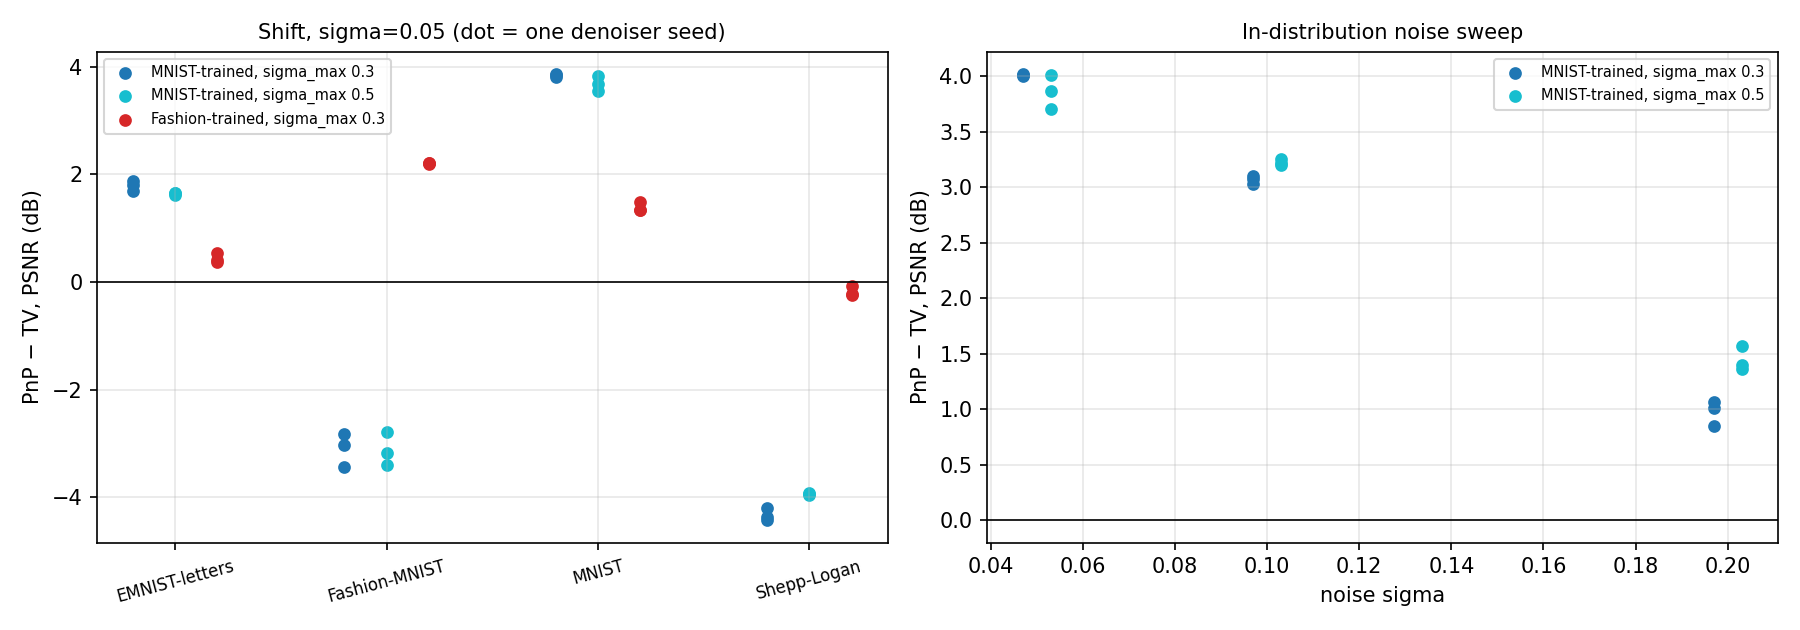
\includegraphics[width=\linewidth]{figures/step4_summary.png}
\caption{Left: PnP$-$TV-ADMM gap for each denoiser seed (dots) on the four test sets, for three priors. Right: gap in the
in-distribution noise sweep for MNIST-trained denoisers with $\sigma_{\max}=0.3$ and $0.5$. Produced by
\texttt{summarize\_step4.py} from \texttt{results/step4/}.}\label{fig:seeds}
\end{figure}


\subsection{E9: Lesion insertion}\label{sec:lesion-results}
Table~\ref{tab:lesion} and Figure~\ref{fig:lesion-summary} summarise the lesion experiment (three denoisers per prior,
protocol of Section~\ref{sec:lesion}; $157$--$197$ valid images per lesion type). TV denotes the ADMM implementation used throughout
the paper; TV-box is the same comparison with the constraint $0\le x\le1$, re-tuned on the same validation split (m03 and f03 families,
same lesion locations and noise seeds). Three observations hold across lesion types.

\emph{TV detects small lesions better than PnP, in distribution and for a matched prior.} For the MNIST-trained prior on MNIST
the paired AUC of PnP is $0.04$--$0.23$ below TV's (for example $0.69$ versus $0.91$ for $\sigma_l=0.75$, $c=0.5$), although
PnP is about $4$\,dB better in PSNR on the same images; for the matched Fashion-trained prior the deficit is $0.03$--$0.17$. The
two methods tie only for the largest high-contrast lesion. Against TV-box the deficit is the same size ($0.00$--$0.22$ on MNIST,
$0.03$--$0.15$ for the matched prior), so the box constraint does not explain it. FBP and Tikhonov also detect small lesions better
than PnP (paired AUC $0.92$ at $\sigma_l=0.75$, $c=0.5$ on MNIST for FBP), at the cost of many false blobs (up to $6$ per image
for FBP).

\emph{In distribution PnP attenuates lesions and invents none.} Its retention is $0.12$--$0.78$ for the MNIST prior on MNIST
and $0.16$--$0.49$ for the matched prior (TV: $0.29$--$0.88$ and $0.38$--$0.83$; TV-box: $0.31$--$0.92$ and $0.33$--$0.82$), and it
produces at most $0.01$ false lesions per image against up to $0.26$ for TV and, for the MNIST-tuned TV-box, up to $0.49$
(smallest low-contrast lesion; $0.075$ for the Fashion-tuned TV-box). The reconstructions are cleaner than TV's but the inserted lesion is often absent
(Figure~\ref{fig:lesion-examples}), so a visually convincing image does not imply a faithful one.

\emph{Under prior mismatch PnP invents structure, but box-constrained TV does too for the smallest lesions.} For the MNIST-trained
prior on Fashion-MNIST the retention is $0.78$--$1.04$ (the lesion survives) but there are $0.20$--$0.66$ false lesions per image
against $\le0.20$ for TV, and the paired AUC remains below TV's by $0.05$--$0.16$. The matched Fashion-trained prior on the same
images produces at most $0.01$. The box-constrained TV is a stricter comparison here: its false-lesion rate on the shifted images is $0.005$--$0.48$ per image, and for
the smallest low-contrast lesion type ($\sigma_l=0.5$, $c=0.25$) it exceeds PnP's ($0.48$ versus $0.38$). For the other seven lesion types PnP's rate is higher, by a factor
of $1.4$ to $50$. The claim that a mismatched learned prior invents more
structure than the classical regulariser therefore holds for TV-box on seven of eight lesion types, not on all of them.
Lesion observability (Section~\ref{sec:lesion}) does not explain these differences: the observability terciles formed within each
lesion type have mean observability $0.88$, $0.92$ and $0.94$, and PnP's paired AUC does not increase with observability (on MNIST
it falls from $0.82$ in the lowest to $0.67$ in the highest tercile); smaller lesions are harder for all methods, but this is
confounded with size.

\begin{table}[htbp]
\centering\small\setlength{\tabcolsep}{3pt}
\caption{Lesion insertion, mean over three denoisers per prior (200 test images, $\sigma=0.05$, 20 angles, bicubic data), for two
of the eight lesion types ($\sigma_l/c$ = lesion size in px / contrast). pAUC: paired AUC; Ret.: retention; FL: false lesions per
lesion-absent image; TV-box: TV with $0\le x\le1$. All methods use their PSNR-tuned settings.}\label{tab:lesion}
\begin{tabular}{llccccccccc}
\toprule
 & & \multicolumn{3}{c}{pAUC} & \multicolumn{3}{c}{Ret.} & \multicolumn{3}{c}{FL}\\
\cmidrule(lr){3-5}\cmidrule(lr){6-8}\cmidrule(lr){9-11}
Prior $\to$ test set & $\sigma_l/c$ & TV & box & PnP & TV & box & PnP & TV & box & PnP\\
\midrule
MNIST $\to$ MNIST (in-dist.)       & 0.75/0.5  & 0.91 & 0.90 & 0.69 & 0.59 & 0.65 & 0.28 & 0.005 & 0.010 & 0.000\\
                                   & 1.25/0.25 & 0.90 & 0.90 & 0.69 & 0.62 & 0.67 & 0.30 & 0.005 & 0.010 & 0.000\\
MNIST $\to$ Fashion (shifted)      & 0.75/0.5  & 0.91 & 0.92 & 0.82 & 0.63 & 0.74 & 0.99 & 0.030 & 0.090 & 0.430\\
                                   & 1.25/0.25 & 0.93 & 0.91 & 0.76 & 0.59 & 0.69 & 0.87 & 0.030 & 0.095 & 0.428\\
Fashion $\to$ Fashion (in-dist.)   & 0.75/0.5  & 0.91 & 0.90 & 0.75 & 0.63 & 0.55 & 0.22 & 0.030 & 0.025 & 0.005\\
                                   & 1.25/0.25 & 0.93 & 0.93 & 0.80 & 0.59 & 0.54 & 0.23 & 0.030 & 0.025 & 0.005\\
Fashion $\to$ MNIST (shifted)      & 0.75/0.5  & 0.91 & 0.90 & 0.75 & 0.59 & 0.55 & 0.35 & 0.005 & 0.000 & 0.000\\
                                   & 1.25/0.25 & 0.90 & 0.90 & 0.78 & 0.62 & 0.60 & 0.36 & 0.005 & 0.000 & 0.000\\
\bottomrule
\end{tabular}
\end{table}

\begin{figure}[htbp]
\centering
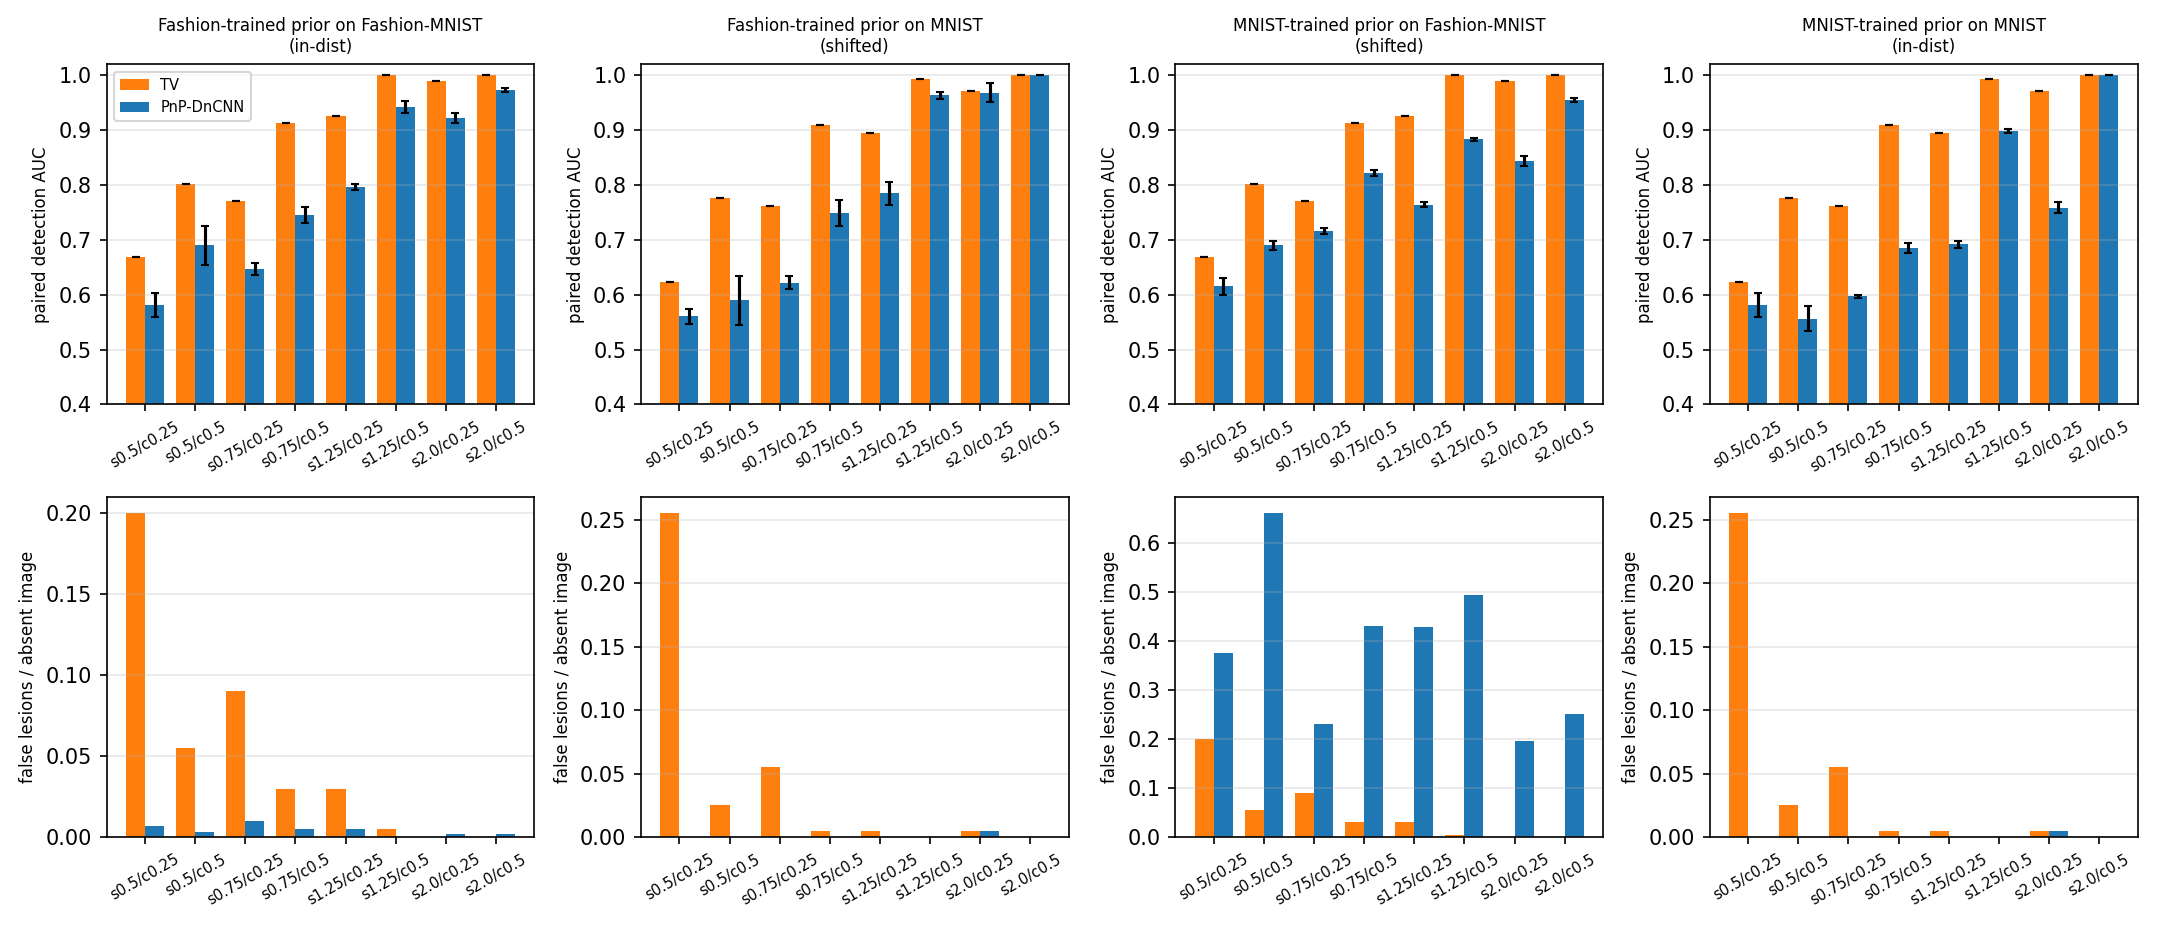
\includegraphics[width=\linewidth]{figures/step5_summary.png}
\caption{Paired detection AUC (top) and false lesions per lesion-absent image (bottom) for TV and PnP-DnCNN in the four
prior/test-set combinations and the eight lesion types (mean over three denoisers; bars: s.d.\ over seeds). TV here is the ADMM
implementation; TV-box values are in Table~\ref{tab:lesion} and \texttt{results/control/}.}\label{fig:lesion-summary}
\end{figure}

\begin{figure}[htbp]
\centering
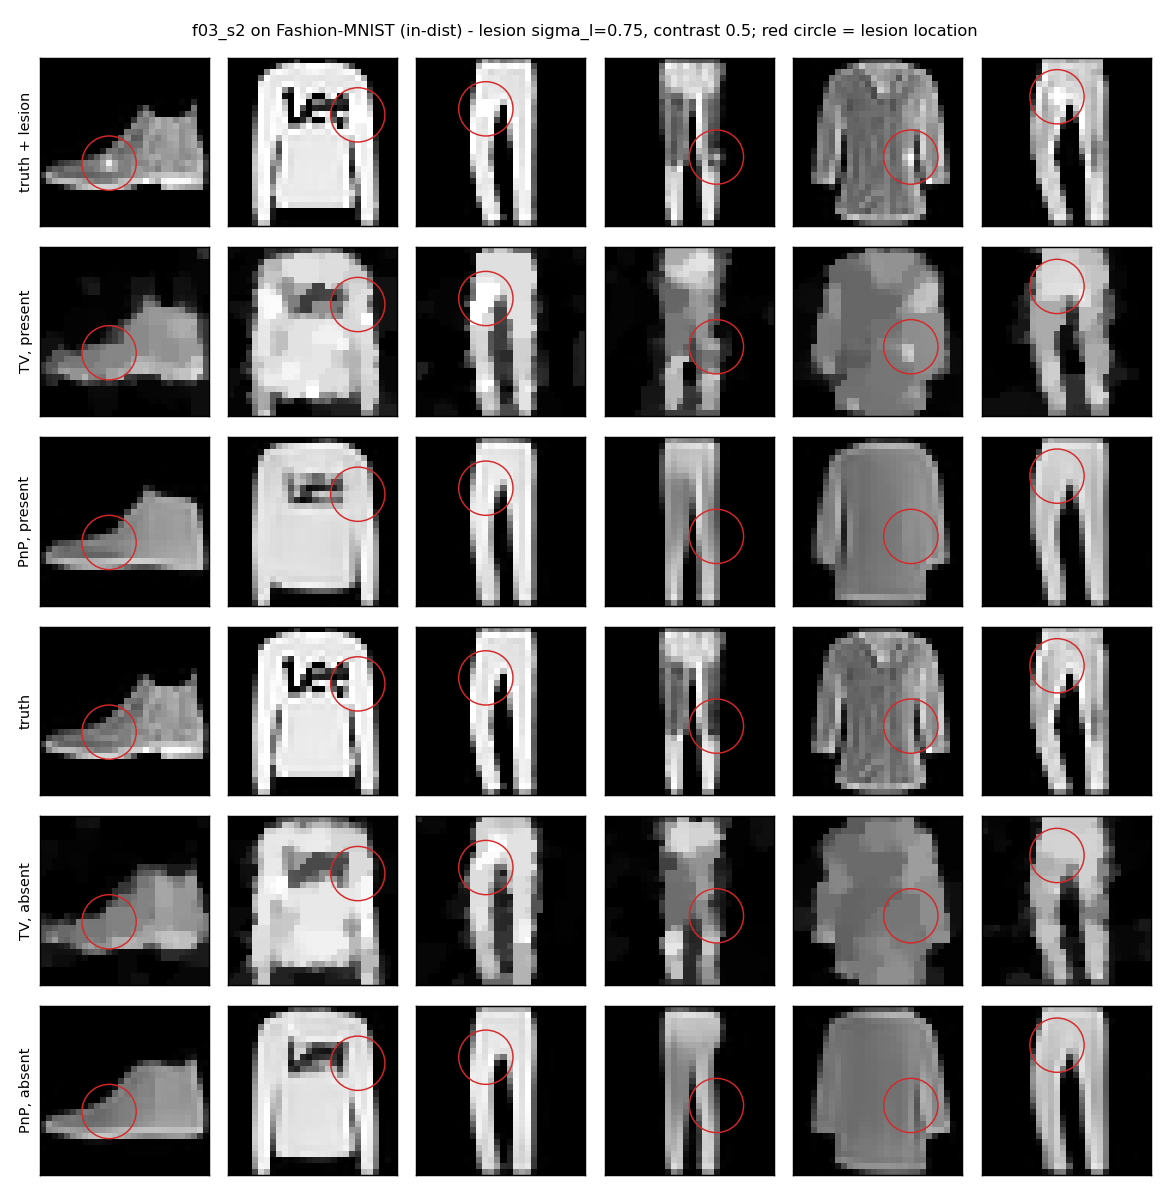
\includegraphics[width=0.85\linewidth]{figures/lesion_f03_s2_examples_fashion.png}
\caption{Matched Fashion-trained prior on Fashion-MNIST ($\sigma_l=0.75$, $c=0.5$). Rows: ground truth with lesion, TV and
PnP reconstructions of the lesion-present image; ground truth, TV and PnP reconstructions of the lesion-absent image. The
red circle marks the lesion location. PnP produces the cleaner images but removes the lesion.}\label{fig:lesion-examples}
\end{figure}

\paragraph{Scope.} The observer is a location-known local-contrast statistic and the lesions are additive Gaussian blobs on
$28\times28$ digits, so these results say how each \emph{reconstruction} preserves or invents a simple signal, not how a human or a
model observer would perform on clinical images. False-lesion counts depend on the response threshold $\theta$, which scales with the
nominal lesion, so they are compared across methods within a lesion type, not across types.


\subsection{E10: Can re-tuning recover lesion detectability?}\label{sec:oppoint-results}
The PSNR-tuned operating point of PnP is not necessarily the best one for lesion detection, so we sweep operating points
(Section~\ref{sec:lesion}) and compare three rules for PnP---PSNR-tuned, best paired AUC on the selection set (``lesion''),
and best paired AUC among points whose selection-set PSNR is at least that of tuned TV (``constrained'')---with TV. All rules are
applied on held-out in-distribution validation images and then reported on the test sets, so no point is chosen on the evaluation images
or with knowledge of the shifted distribution. This experiment uses one denoiser per prior (seed 0 of the m03 and f03 families), the
ADMM implementation of TV, and the two lesion types $\sigma_l=0.75$, $c=0.5$ and $\sigma_l=1.25$, $c=0.25$; neither seed variation nor
the box-constrained TV was examined here. Table~\ref{tab:oppoint} and Figures~\ref{fig:oppoint} and~\ref{fig:oppoint-f} show the results.

\paragraph{MNIST-trained prior, in distribution.} The constrained point keeps a $+0.7$\,dB PSNR advantage over TV (the PSNR-tuned
advantage was $+4.0$\,dB) but its paired AUC is still $0.06$ below TV's (for both lesion types), and its false-lesion rate
rises to 12 times TV's ($0.060$ versus $0.005$ per image). The lesion-tuned point matches TV's detection ($0.916$ versus $0.910$) but has
a lower PSNR than TV ($19.6$ versus $20.1$\,dB) and about 60 times TV's false-lesion rate ($0.32$ versus $0.005$ per image). Tuning TV for
detection instead changes it very little (PSNR $20.13$\,dB, pAUC $0.904$), so TV has no comparable trade-off in this grid. As an upper bound
that uses the test set, the best of the $45$ PnP settings among those with PSNR at least TV's reaches a paired AUC of $0.898$ at $0.28$
false lesions per image, so no rule could have closed the gap for this prior without a large false-lesion cost.

\paragraph{Fashion-trained prior.} In distribution (Fashion-MNIST) the constrained point keeps $+1.0$\,dB over TV with a paired AUC
$0.02$--$0.03$ below TV's and $0.085$ false lesions per image against $0.03$ for TV. A difference of this size is comparable to the
binomial standard error of a paired AUC with $170$--$190$ valid images ($\approx0.02$--$0.03$); we did not compute a paired interval, so we
describe it as close to TV's, not as equal. On the shifted MNIST images the constrained point keeps $+1.0$\,dB, with a paired AUC $0.02$--$0.06$ below TV's and
$0.015$ false lesions per image against $0.005$.

\paragraph{Under mismatch.} Operating points chosen in distribution do not protect the MNIST-trained prior on Fashion-MNIST: all
three rules are $2.1$--$2.8$\,dB below TV in PSNR and produce $0.40$--$0.51$ false lesions per image against $0.03$. This is not an
artefact of the selection rule: none of the $45$ PnP settings in the grid reaches TV's PSNR on the shifted images (the best is $17.96$
versus $19.37$\,dB), even when judged on the test set itself.

\paragraph{Summary.} PSNR, detectability and fabricated structure trade against each other for PnP, and only the Fashion-trained
prior leaves a point at which PnP stays above TV in PSNR with a detection close to TV's and few false lesions. This holds for it on Fashion-MNIST and on
MNIST, i.e.\ for one in-distribution and one shifted test set, but for the MNIST-trained prior it holds on neither test set. The difference between the priors is therefore the breadth of the training
distribution (E8), not whether a test set is formally in-distribution. With one denoiser per prior this is a statement about two networks.

\begin{table}[htbp]
\centering\small\setlength{\tabcolsep}{4pt}
\caption{Operating points for lesion type $\sigma_l=0.75$, $c=0.5$ on the test sets (one denoiser per prior; points chosen on
held-out in-distribution validation images). PSNR is that of the lesion-absent reconstruction. ``TV, lesion'' is TV with the weight
that maximises paired AUC on the selection set.}\label{tab:oppoint}
\begin{tabular}{llccc}
\toprule
Prior $\to$ test set & Operating point & PSNR (dB) & pAUC & FL\\
\midrule
MNIST $\to$ MNIST (in-dist.)     & TV (PSNR-tuned)  & 20.11 & 0.910 & 0.005\\
                                 & TV, lesion       & 20.13 & 0.904 & 0.005\\
                                 & PnP, PSNR-tuned  & 24.07 & 0.693 & 0.000\\
                                 & PnP, constrained & 20.84 & 0.849 & 0.060\\
                                 & PnP, lesion      & 19.57 & 0.916 & 0.315\\
MNIST $\to$ Fashion (shifted)    & TV (PSNR-tuned)  & 19.37 & 0.914 & 0.030\\
                                 & TV, lesion       & 19.33 & 0.924 & 0.035\\
                                 & PnP, PSNR-tuned  & 16.58 & 0.822 & 0.420\\
                                 & PnP, constrained & 17.32 & 0.886 & 0.405\\
                                 & PnP, lesion      & 16.78 & 0.903 & 0.505\\
Fashion $\to$ Fashion (in-dist.) & TV (PSNR-tuned)  & 19.37 & 0.914 & 0.030\\
                                 & TV, lesion       & 18.94 & 0.914 & 0.010\\
                                 & PnP, PSNR-tuned  & 21.58 & 0.751 & 0.005\\
                                 & PnP, constrained & 20.41 & 0.897 & 0.085\\
                                 & PnP, lesion      & 19.07 & 0.870 & 0.255\\
Fashion $\to$ MNIST (shifted)    & TV (PSNR-tuned)  & 20.11 & 0.910 & 0.005\\
                                 & TV, lesion       & 19.06 & 0.916 & 0.000\\
                                 & PnP, PSNR-tuned  & 21.67 & 0.759 & 0.000\\
                                 & PnP, constrained & 21.13 & 0.855 & 0.015\\
                                 & PnP, lesion      & 21.21 & 0.898 & 0.040\\
\bottomrule
\end{tabular}
\end{table}

\begin{figure}[htbp]
\centering
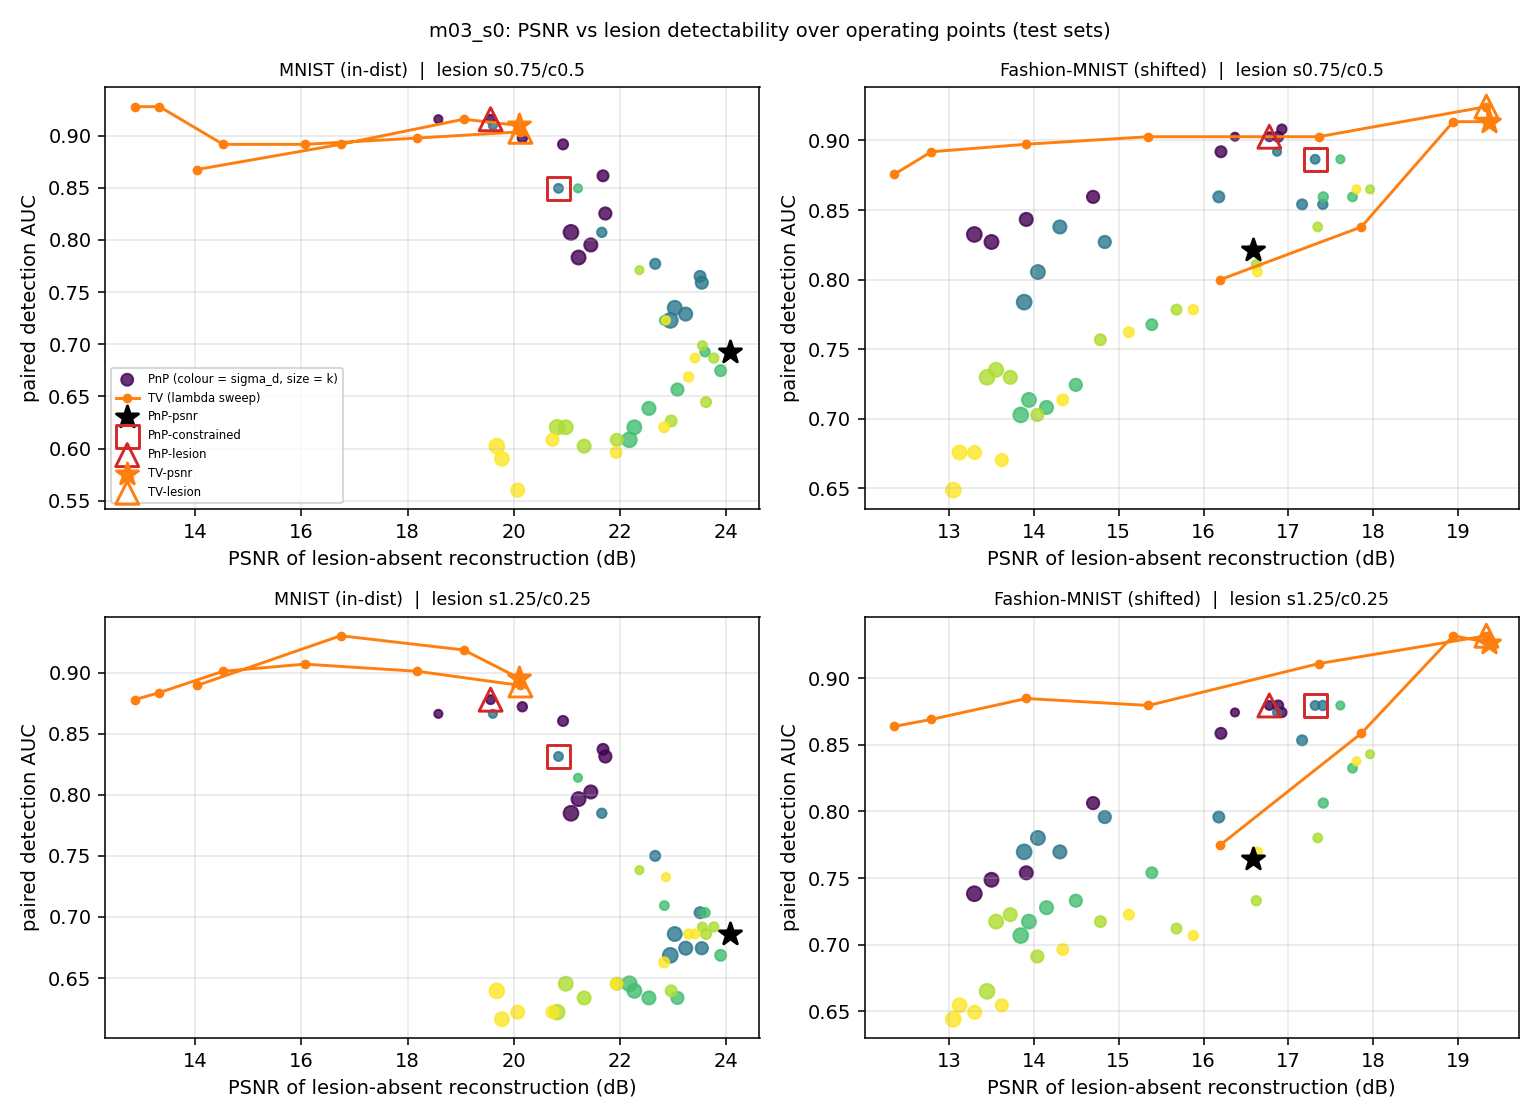
\includegraphics[width=\linewidth]{figures/oppoint_m03_s0.png}
\caption{PSNR of the lesion-absent reconstruction versus paired detection AUC over all operating points of PnP (colour:
$\sigma_d$; marker size: iterations) and TV (line: weight sweep) for the MNIST-trained denoiser. Markers show the selected
operating points. Left: in distribution; right: Fashion-MNIST (shifted).}\label{fig:oppoint}
\end{figure}

\begin{figure}[htbp]
\centering
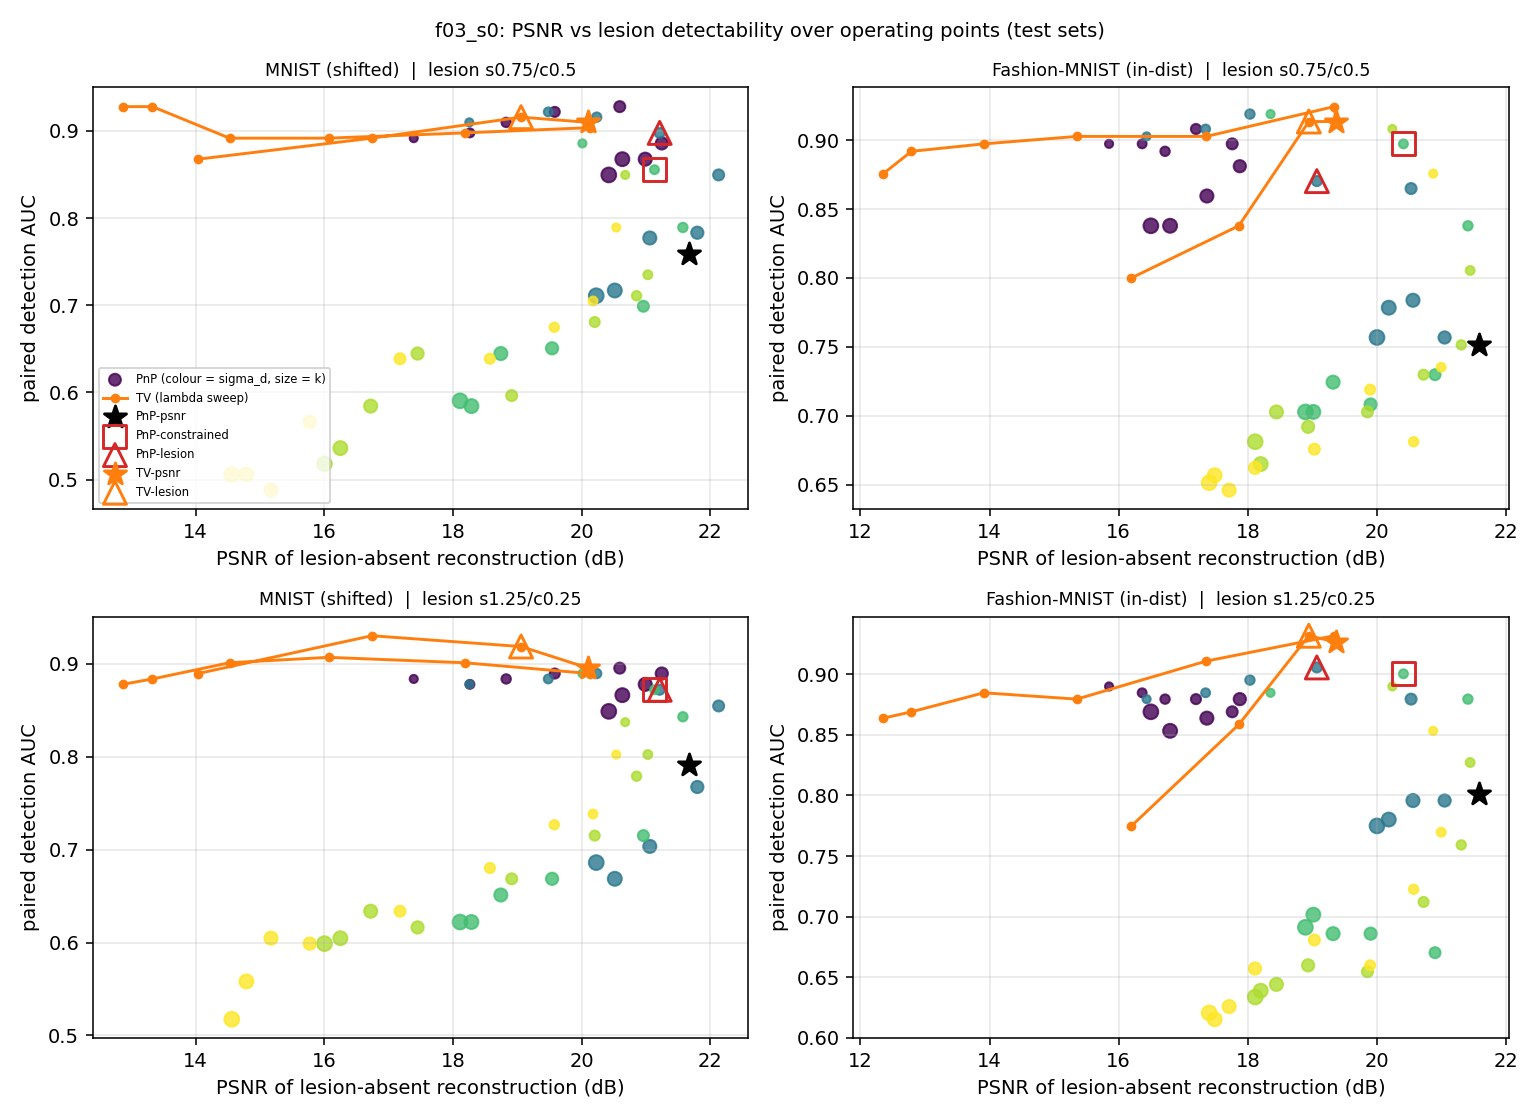
\includegraphics[width=\linewidth]{figures/oppoint_f03_s0.png}
\caption{As Figure~\ref{fig:oppoint} for the Fashion-trained denoiser. Left: MNIST (shifted); right: Fashion-MNIST (in distribution).
Both figures are produced by \texttt{run\_oppoint.py}.}\label{fig:oppoint-f}
\end{figure}


\subsection{E11: The matrix-free operator reproduces the dense pipeline}\label{sec:mf-results}
Table~\ref{tab:mf} compares the two implementations on the same 200 noisy test images ($\sigma=0.05$, 20 angles, bicubic
fine-grid data). The comparison uses fixed, untuned settings (Tikhonov and TV weight $10^{-2}$; PnP with $\sigma_d=0.1$ and $k=25$), so its PSNR values
are not comparable to the tuned values of E1--E2; only the agreement between the two implementations matters here.
The projections agree to $3\times10^{-7}$ in relative norm, and the three reconstruction methods agree to
$\le10^{-5}$ (Tikhonov, TV) and $3\times10^{-4}$ (PnP) in relative norm, with identical PSNR to three decimals. The slightly larger PnP difference
is plausible given that the denoiser is applied $25$ times to slightly different iterates, but we did not isolate its source.

The randomized SVD reproduces the singular values of the dense SVD to within $1.1\times10^{-4}\,s_1$ for the first $400$ and
$6.2\times10^{-5}\,s_1$ for the first $600$ (the number used to build the subspace in E7). It finds the same $465$-dimensional well-determined
subspace $\{i:s_i/s_1\ge0.05\}$ (so $319$ directions are weakly determined). The resulting strong/weak error split differs from the dense one by at most
$2.3\times10^{-4}$ of the error norm for each of the three methods (Tikhonov, TV-ADMM, PnP), far below the $1\%$ tolerance of the unit test; the strong subspace holds
$91\%$, $82\%$ and $77\%$ of the squared error of the three reconstructions, respectively. These checks are produced by \texttt{run\_e11\_svd\_check.py} and
are limited by single-precision arithmetic on the GPU.

At this size the dense implementation is much faster for the iterative solvers (Table~\ref{tab:mf}): the matrix-free TV-ADMM
performs $100$ ADMM iterations with up to $30$ conjugate-gradient steps each, i.e.\ up to $3\times10^{3}$ forward--adjoint pairs per
image, and the adjoint is evaluated by reverse-mode differentiation. PnP is only $1.2$ times slower because the denoiser dominates its cost.
The timings are single runs on one GPU (RTX 3050 Ti) and should be read as orders of magnitude. The matrix-free operator is therefore a requirement for larger images, where the dense matrix cannot be stored,
rather than an optimisation at $28\times28$.

\begin{table}[htbp]
\centering\small\setlength{\tabcolsep}{4pt}
\caption{Dense versus matrix-free pipeline (200 images, fixed untuned settings, single GPU run). Rel.\ diff.: relative difference between
the two reconstructions. Peak GPU memory for the whole comparison: 184\,MB.}\label{tab:mf}
\begin{tabular}{lcccc}
\toprule
Method & Rel.\ diff. & PSNR (dense = MF) & Time dense (s) & Time MF (s)\\
\midrule
Tikhonov & $4.6\times10^{-6}$ & 16.36 & 0.08 & 0.26\\
TV-ADMM  & $9.7\times10^{-6}$ & 19.01 & 0.16 & 7.50\\
PnP ($k=25$) & $2.8\times10^{-4}$ & 23.10 & 0.76 & 0.94\\
\bottomrule
\end{tabular}
\end{table}


\subsection{E12: Poisson dose sweep}\label{sec:dose-results}
Table~\ref{tab:dose} and Figure~\ref{fig:dose} give the PnP--TV difference over the dose range (200 test images per set; the
Shepp--Logan phantom is one image with one noise draw per dose, so it has no interval). Settings are those of Section~\ref{sec:poisson}: tuned on MNIST
validation images at each dose, unweighted data term, ADMM implementation of TV, and one MNIST-trained denoiser. The qualitative picture of
Stage~1 is reproduced; every interval for the 200-image sets excludes zero by at least $6$ standard errors.

\emph{Prior-matched data.} On MNIST the learned prior beats TV at every dose, by $+3.7$\,dB at $I_0=100$--$300$ (effective $\sigma\approx0.03$--$0.06$), against $+3.84$\,dB at Gaussian $\sigma=0.05$,
and for 99--100\% of the images at $I_0\ge100$. The advantage shrinks at both ends of the dose range, to $+0.8$\,dB at $I_0=10$, of the same order as the Gaussian result at $\sigma=0.2$
($+0.97$\,dB, E8). EMNIST keeps a smaller advantage ($+0.6$ to $+1.8$\,dB). These gaps are against TV without the box constraint; that constraint was not tested
under Poisson noise (in the Gaussian MNIST case it lowered the gap by $0.5$\,dB, E8).

\emph{Shifted data.} The MNIST-trained prior is below TV on Fashion-MNIST ($-2.0$ to $-3.1$\,dB; PnP wins on only 6--14\% of the images)
and on the phantom ($-4.4$ to $-6.1$\,dB), as in Stage~1 ($-3.10$ and $-4.33$\,dB). At $I_0=1000$ the prior is no better than FBP on Fashion-MNIST
($19.72$ versus $19.77$\,dB), and on the phantom it is $3.1$\,dB below FBP ($18.07$ versus $21.20$\,dB).
The share of the error in the complement of the well-determined subspace is $0.68$--$0.99$ of TV's on MNIST but $1.04$--$1.19$ on Fashion-MNIST
and $1.73$--$1.79$ on the phantom (for $I_0\le300$; $0.90$ at $I_0=1000$), so the mismatch error again sits partly in the weakly determined directions. These ratios are less favourable to PnP than the
Stage~1 values and are not directly comparable, since the noise model, the tuned settings and the subspace definition differ. The gap on Fashion-MNIST is not monotone in dose
($-2.45$, $-3.05$, $-2.74$, $-3.01$, $-1.98$\,dB from high to low dose); with frozen MNIST-tuned settings this reflects, at least in part, the choice of $(\sigma_d,k)$ (see the weighted variant below), so
we read the Fashion-MNIST range as ``$2$ to $3$\,dB below TV'' and not as a dose trend.

\emph{Structural similarity.} In SSIM the picture differs on Fashion-MNIST (Table~\ref{tab:dosessim}): the PnP--TV difference is between $-0.014$ and $+0.054$ and PnP wins on
$47$--$67$\% of the images, so the $2$--$3$\,dB PSNR reversal has no counterpart in SSIM. On the phantom SSIM is lower for PnP at every dose ($-0.19$ to $-0.31$). On MNIST and EMNIST PnP is better in SSIM at every dose.
The reversal under shift is therefore a PSNR result for Fashion-MNIST and a PSNR and SSIM result for the phantom.

\emph{Weighted data term.} Using the Poisson weights in PnP gave no consistent benefit: the weighted variant was $0.14$--$0.59$\,dB below the unweighted one in 13 of the 15 non-phantom
cells, and above it in two (EMNIST $+0.35$\,dB and Fashion-MNIST $+1.10$\,dB at $I_0=300$), where the tuned $(\sigma_d,k)$ differed ($(0.05,10)$ unweighted versus $(0.1,3)$ weighted). The
$1.1$\,dB on Fashion-MNIST shows that the shifted-data gap depends on how the frozen settings were chosen. We report the unweighted scheme, as it is the one tuned on the same footing as in Stage~1, and note that the weighted variant would reduce the
Fashion-MNIST gap at $I_0=300$ from $-3.05$ to about $-1.95$\,dB.

\begin{table}[htbp]
\centering\small\setlength{\tabcolsep}{4pt}
\caption{PnP$-$TV PSNR difference (dB, mean $\pm$ standard error of the paired difference over 200 images) by photon count $I_0$, with the corresponding
effective sinogram noise standard deviation (measured on the MNIST images; signal dependence makes it about $15$--$20\%$ higher on Fashion-MNIST); and the ratio of PnP's to TV's reconstruction error in the complement of the well-determined subspace (in brackets). Phantom: one image.}\label{tab:dose}
\resizebox{\linewidth}{!}{%
\begin{tabular}{lccccc}
\toprule
$I_0$ (photons/ray) & 1000 & 300 & 100 & 30 & 10\\
effective $\sigma$ & 0.018 & 0.032 & 0.056 & 0.106 & 0.198\\
\midrule
MNIST (train dist.) & $+2.87\pm.07$ (0.70) & $+3.68\pm.08$ (0.68) & $+3.65\pm.08$ (0.71) & $+2.39\pm.12$ (0.88) & $+0.82\pm.12$ (0.99)\\
EMNIST              & $+1.40\pm.09$ (0.75) & $+1.59\pm.08$ (0.83) & $+1.82\pm.08$ (0.86) & $+0.77\pm.11$ (1.02) & $+0.62\pm.10$ (1.00)\\
Fashion-MNIST       & $-2.45\pm.13$ (1.04) & $-3.05\pm.16$ (1.18) & $-2.74\pm.16$ (1.18) & $-3.01\pm.14$ (1.19) & $-1.98\pm.13$ (1.07)\\
Shepp--Logan        & $-4.41$ (0.90) & $-6.05$ (1.79) & $-5.05$ (1.73) & $-5.49$ (1.77) & $-4.75$ (1.75)\\
\bottomrule
\end{tabular}}
\end{table}

\begin{table}[htbp]
\centering\small\setlength{\tabcolsep}{4pt}
\caption{PnP$-$TV SSIM difference (mean $\pm$ standard error over 200 images; share of images won by PnP in brackets) for the same runs as Table~\ref{tab:dose}.}\label{tab:dosessim}
\resizebox{\linewidth}{!}{%
\begin{tabular}{lccccc}
\toprule
$I_0$ (photons/ray) & 1000 & 300 & 100 & 30 & 10\\
\midrule
MNIST (train dist.) & $+.089\pm.002$ (1.00) & $+.170\pm.005$ (1.00) & $+.244\pm.006$ (1.00) & $+.279\pm.008$ (1.00) & $+.267\pm.009$ (0.99)\\
EMNIST              & $+.039\pm.002$ (0.96) & $+.081\pm.003$ (0.99) & $+.123\pm.004$ (1.00) & $+.136\pm.006$ (0.98) & $+.166\pm.007$ (0.98)\\
Fashion-MNIST       & $-.014\pm.007$ (0.47) & $-.005\pm.009$ (0.50) & $+.026\pm.010$ (0.55) & $+.011\pm.009$ (0.52) & $+.054\pm.009$ (0.67)\\
Shepp--Logan        & $-.216$ & $-.306$ & $-.189$ & $-.245$ & $-.206$\\
\bottomrule
\end{tabular}}
\end{table}

\begin{figure}[htbp]
\centering
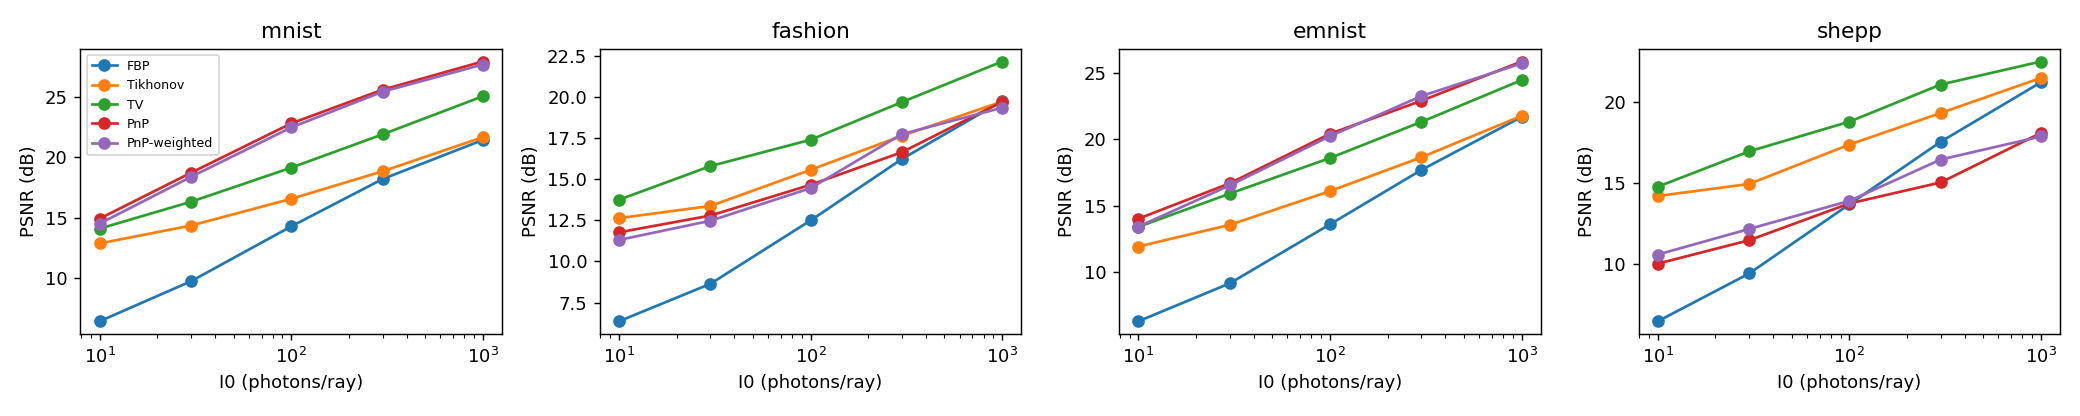
\includegraphics[width=\linewidth]{figures/dose_sweep.png}
\caption{PSNR versus photon count for FBP, Tikhonov, TV, PnP and the Poisson-weighted PnP on the four test sets (MNIST-trained denoiser,
hyperparameters tuned on MNIST validation images at each dose).}\label{fig:dose}
\end{figure}


\subsection{E13: Lesion insertion under Poisson noise}\label{sec:lesion-poisson}
We repeated the lesion experiment (Section~\ref{sec:lesion}; same lesions, observer, locations and validity filter; three denoisers per prior, 200 images per set) with
Poisson data at $I_0=100$ and $I_0=30$ (effective $\sigma\approx0.06$ and $0.1$) and the matrix-free operator, tuning each method on its prior's own validation distribution
(Table~\ref{tab:lesion-poisson}, Figure~\ref{fig:lesion-poisson}). TV is the ADMM implementation without the box constraint; the box-constrained control of E9 was run for Gaussian noise
only. Only these two doses were run; the other three doses of E12 were not.
 
\emph{Erasure persists.} The paired AUC of PnP is below TV's in all four prior/test-set combinations and at both doses (differences of $-0.01$ to $-0.28$ at $I_0=100$, with one tie at $1.0$ for the largest high-contrast lesion, and $-0.02$ to $-0.19$ at $I_0=30$). For the MNIST prior on MNIST ($\sigma_l=0.75$, $c=0.5$) the paired AUC is $0.60$ against $0.89$ for TV and the retention is $0.29$ against $0.60$ at $I_0=100$,
which is close to the Gaussian-noise values of Stage~1 ($0.69$ vs.\ $0.91$; $0.28$ vs.\ $0.59$), although PnP is $3.7$\,dB better in PSNR on the same images. At $I_0=30$ the gap narrows
($0.63$ vs.\ $0.77$) because TV degrades faster.
 
\emph{Invention under mismatch persists.} For the MNIST-trained prior on Fashion-MNIST, PnP produces more false lesions than TV for lesions with $\sigma_l\ge0.75$ in 11 of the 12 dose/lesion-type cells, by factors of $1.7$--$5.5$ ($0.25$--$0.70$ against $0.06$--$0.28$ per image at $I_0=100$; the exception is $0.25$ against $0.28$). The matched Fashion-trained prior, on its own data and on MNIST, stays at $\le0.09$ false lesions per image. Retention above that of TV
for the mismatched prior should not be read as fidelity: invented contrast may contribute to it, although we did not separate the two.
 
\emph{New at the lower dose: in-distribution invention.} For the MNIST prior on MNIST at $I_0=30$, PnP produces $0.058$--$0.073$ false lesions per image for the four lesion types with $0.75\le\sigma_l\le1.25$, against $0.000$--$0.035$ for TV,
whereas at $I_0=100$ it produces at most $0.01$ for any type. At high noise the in-distribution prior therefore starts to create lesion-like structure as well as to erase it, although at a rate far below that under mismatch.
 
\emph{TV has a failure of its own.} For the smallest low-contrast lesion at $I_0=100$ the TV reconstruction contains $0.63$ false lesions per image (noise blobs), against $0.01$ for PnP. The statement that PnP creates more false lesions than TV under mismatch therefore applies to lesions of $\sigma_l\ge0.75$\,px, and under a matched prior is not supported at all. As in E9, where box-constrained TV also produced false lesions for the smallest lesion type, the false-lesion rate of TV depends on its implementation, so
the TV false-lesion counts here are those of ADMM-TV and may be different for other TV solvers.
 
Uncertainty is limited by the design: the error bars in Figure~\ref{fig:lesion-poisson} show the variation over three denoisers only, TV is a single run, and with about 170 valid lesions per cell the sampling error of a paired AUC is of the order of $\pm0.03$, so differences below that, such as the ties for the
largest lesions, do not separate the methods. A tercile analysis of PnP's paired AUC by lesion observability showed a decrease with observability on MNIST images and no trend on Fashion-MNIST images; since it depends on the image set, our hypothesis is that it reflects the background around the lesion rather than the operator; we did not test this and do not interpret it
(the same pattern appears in the Gaussian-noise data of E9).
 
\begin{table}[htbp]
\centering\small\setlength{\tabcolsep}{3pt}
\caption{Lesion insertion under Poisson noise, mean over three denoisers per prior (200 test images; 20 angles; bicubic data), for two of the eight lesion types.
pAUC: paired AUC; Ret.: retention; FL: false lesions per lesion-absent image. Each method is tuned on its own prior's validation distribution at the given dose.}\label{tab:lesion-poisson}
\resizebox{\linewidth}{!}{%
\begin{tabular}{llcccccccccccc}
\toprule
 & & \multicolumn{6}{c}{$I_0=100$} & \multicolumn{6}{c}{$I_0=30$}\\
\cmidrule(lr){3-8}\cmidrule(lr){9-14}
 & & \multicolumn{2}{c}{pAUC} & \multicolumn{2}{c}{Ret.} & \multicolumn{2}{c}{FL} & \multicolumn{2}{c}{pAUC} & \multicolumn{2}{c}{Ret.} & \multicolumn{2}{c}{FL}\\
\cmidrule(lr){3-4}\cmidrule(lr){5-6}\cmidrule(lr){7-8}\cmidrule(lr){9-10}\cmidrule(lr){11-12}\cmidrule(lr){13-14}
Prior $\to$ test set & $\sigma_l/c$ & TV & PnP & TV & PnP & TV & PnP & TV & PnP & TV & PnP & TV & PnP\\
\midrule
MNIST $\to$ MNIST    & 0.75/0.5  & .89 & .60 & .60 & .29 & .010 & .007 & .77 & .63 & .48 & .34 & .005 & .067\\
                     & 1.25/0.25 & .88 & .60 & .60 & .27 & .020 & .007 & .75 & .65 & .46 & .46 & .005 & .068\\
MNIST $\to$ Fashion  & 0.75/0.5  & .81 & .72 & .64 & .84 & .240 & .443 & .73 & .63 & .42 & .57 & .230 & .518\\
                     & 1.25/0.25 & .84 & .72 & .65 & .84 & .255 & .438 & .71 & .61 & .42 & .54 & .225 & .518\\
Fashion $\to$ Fashion & 0.75/0.5 & .79 & .64 & .46 & .23 & .075 & .020 & .69 & .58 & .25 & .11 & .020 & .038\\
                     & 1.25/0.25 & .85 & .71 & .48 & .25 & .075 & .020 & .68 & .56 & .27 & .16 & .040 & .038\\
Fashion $\to$ MNIST  & 0.75/0.5  & .88 & .66 & .48 & .31 & .000 & .003 & .78 & .64 & .33 & .27 & .000 & .007\\
                     & 1.25/0.25 & .89 & .66 & .49 & .33 & .000 & .003 & .78 & .65 & .34 & .34 & .000 & .007\\
\bottomrule
\end{tabular}}
\end{table}
 
\begin{figure}[htbp]
\centering
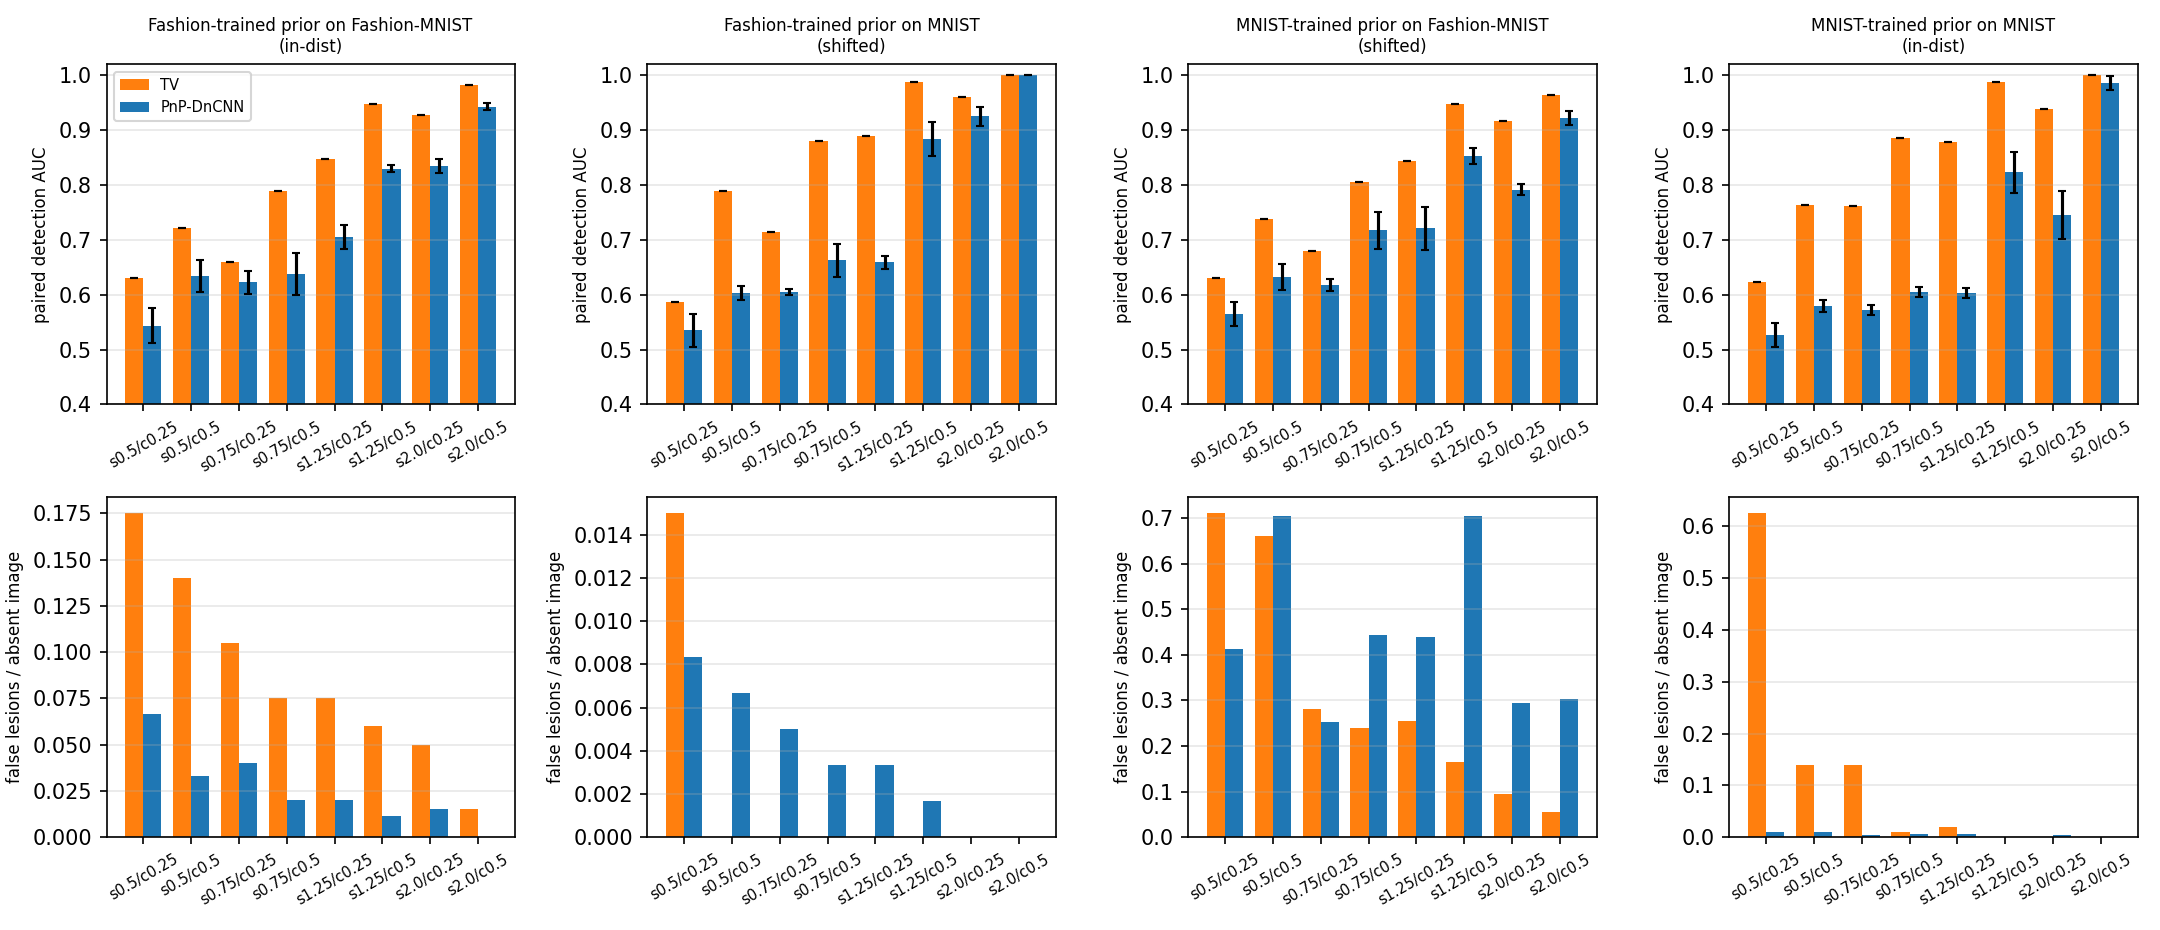
\includegraphics[width=\linewidth]{figures/step5_summary_lesions_I100.png}\\[2pt]
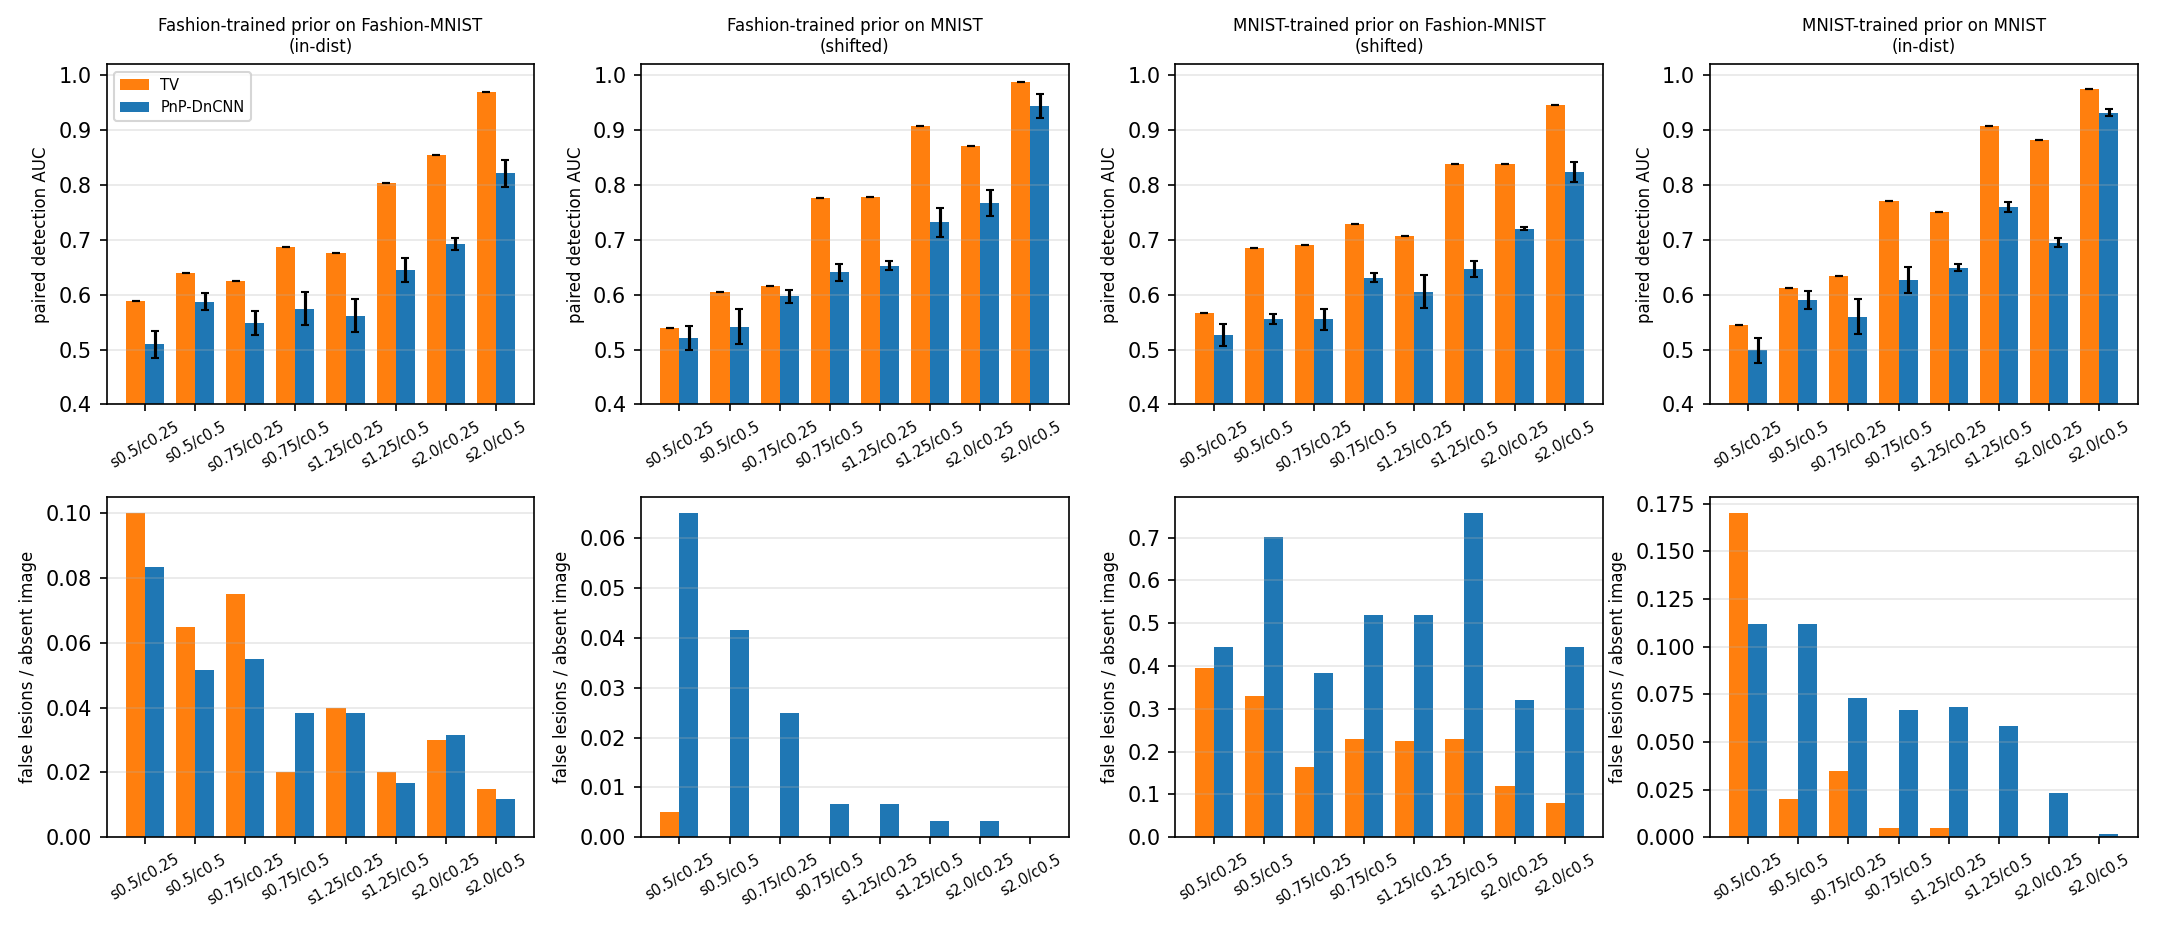
\includegraphics[width=\linewidth]{figures/step5_summary_lesions_I30.png}
\caption{Paired detection AUC (top rows) and false lesions per lesion-absent image (bottom rows) under Poisson noise, $I_0=100$ (upper panel) and $I_0=30$ (lower panel). Bars: mean over three
denoisers; error bars: s.d.\ over seeds.}\label{fig:lesion-poisson}
\end{figure}


\subsection{E14: Data, noise model and simulator}\label{sec:e14}
The geometry fit, the noise-model checks and the dose thinning are described in Sections~\ref{sec:lodopab}--\ref{sec:sim3}. Figure~\ref{fig:geom} illustrates the geometry fit of Section~\ref{sec:lodopab} for one test slice. All hyperparameters are tuned on \emph{real} (thinned) observations of
the validation slices, whereas every reported comparison is evaluated on \emph{simulated} crime-free data of the test slices. The simulator therefore has to be shown to be a faithful stand-in for the real data, and
Table~\ref{tab:simcheck} does this for the baseline that is cheapest to run: it compares the TV PSNR obtained from the real (thinned) observations with that obtained from our crime-free simulation of the same slices.
The agreement is within $0.15$\,dB at all nine conditions (first 8 test slices, one noise realisation each; mean difference $+0.03$\,dB, simulated minus real). For all 40 slices at $K=60$ the values are $31.91$ vs.\ $32.04$\,dB (full dose) and
$29.82$ vs.\ $29.83$\,dB (quarter dose), and for FBP-Hann $30.65$ vs.\ $30.59$ and $28.73$ vs.\ $28.66$\,dB.

The residual differences are small compared with the method differences studied below ($\le2.3$\,dB), but they are not zero and they are not random in sign across doses: the simulation is slightly \emph{easier} than the real data
at full dose ($+0.07$ to $+0.15$\,dB at all three $K$), and indistinguishable or slightly harder at the two lower doses ($-0.05$ to $+0.05$\,dB). This is the direction expected if the real counts carry somewhat
more variance than the simulation at high counts (dispersion index in Section~\ref{sec:sim3}), but it is a hypothesis: eight slices and a single noise draw do not allow a test, and we did not compute an interval for these differences.
What the check does \emph{not} show is that the \emph{difference} between PnP and TV is the same on real and simulated data, only that the TV baseline is; we therefore state the PnP--TV comparisons for the simulated data and treat the
simulator as validated for baseline accuracy, not for every method.

\begin{figure}[htbp]
\centering
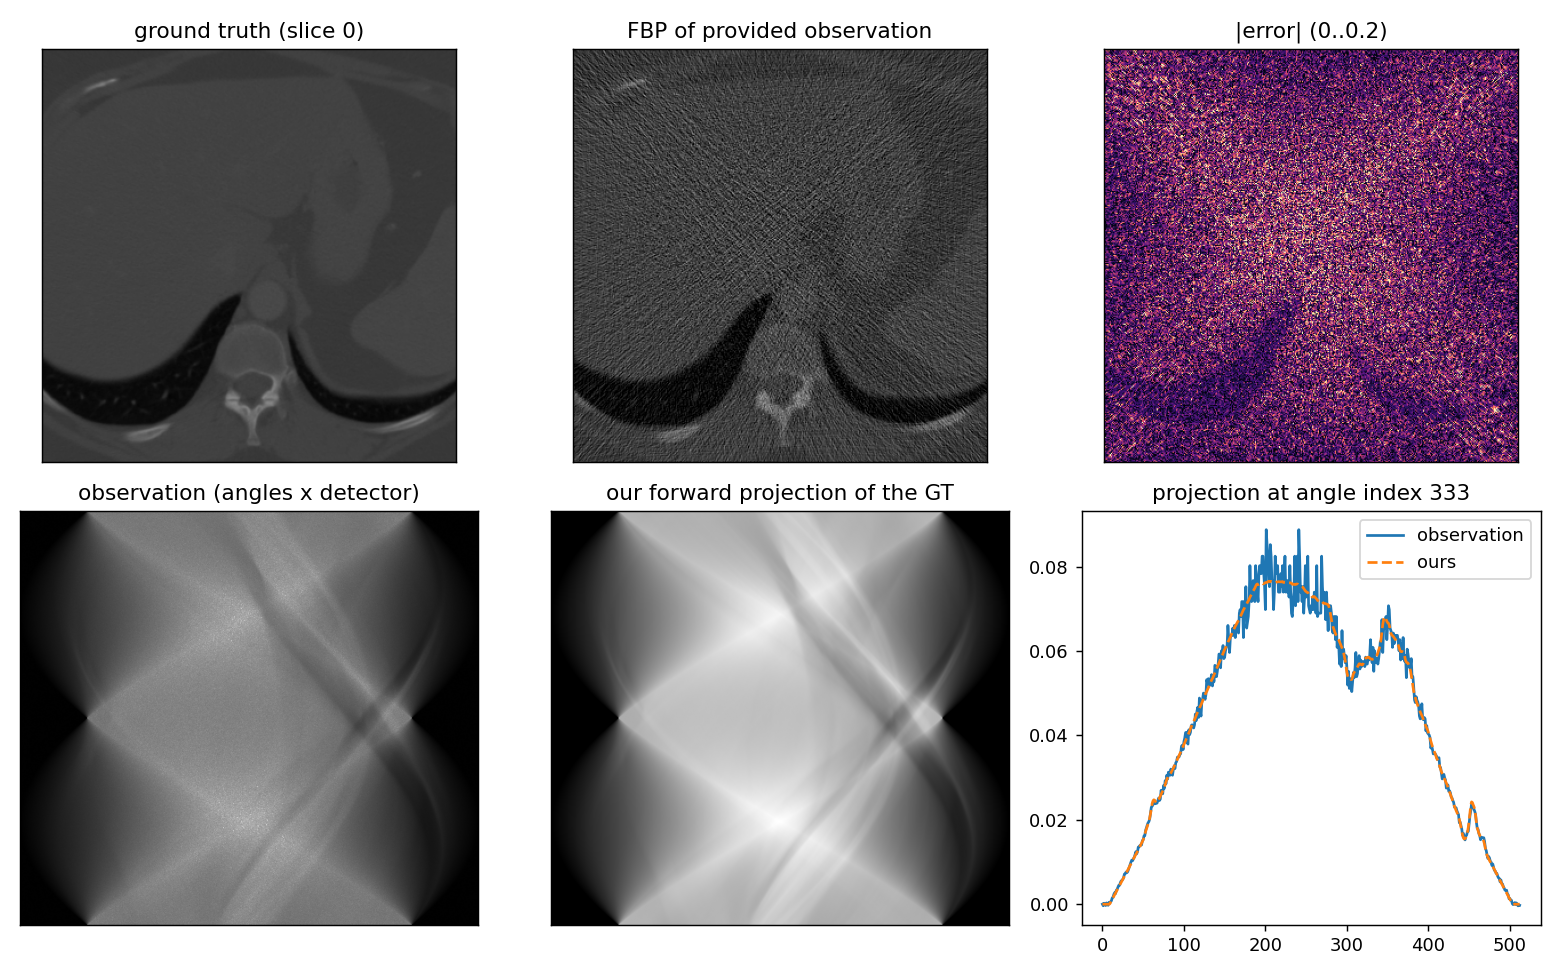
\includegraphics[width=\linewidth]{figures/geometry_check.png}
\caption{Geometry check on one slice (slice 0). Top: ground truth, FBP of the supplied observation, and the absolute error of that FBP. Bottom: the supplied sinogram, our forward projection of the ground truth, and one projection (angle index 333) of the observation (solid) and of our projection (dashed). The observation is the noisy version of our noise-free projection, with matching structure. The fit statistics (relative residual $0.038$, correlation $0.9979$, with a fitted least-squares scale) are pooled over 8 evenly spaced test slices (Section~\ref{sec:lodopab}); the figure shows only the first of them.}\label{fig:geom}
\end{figure}

\begin{table}[htbp]
\centering\small\setlength{\tabcolsep}{5pt}
\caption{TV PSNR (dB) from real observations (thinned to the dose, subsampled to $K$ angles) and from the crime-free simulation of the same slices (first 8 test slices).}\label{tab:simcheck}
\begin{tabular}{llccccccccc}
\toprule
$K$ & & \multicolumn{3}{c}{30} & \multicolumn{3}{c}{60} & \multicolumn{3}{c}{120}\\
\cmidrule(lr){3-5}\cmidrule(lr){6-8}\cmidrule(lr){9-11}
dose & & 1 & 0.25 & 0.1 & 1 & 0.25 & 0.1 & 1 & 0.25 & 0.1\\
\midrule
real & & 29.34 & 27.95 & 26.57 & 30.15 & 28.40 & 26.73 & 30.61 & 28.54 & 27.89\\
simulated & & 29.41 & 27.90 & 26.52 & 30.27 & 28.45 & 26.72 & 30.76 & 28.55 & 27.85\\
\bottomrule
\end{tabular}
\end{table}
 
\begin{table}[htbp]
\centering\small\setlength{\tabcolsep}{4pt}
\caption{Tuned parameters (20 validation slices per condition): Hann cut-off, TV weight (the TV-long weight was the same in every condition), and $(\sigma_d,k)$ of PnP-const and PnP-TVinit.}\label{tab:params3}
\begin{tabular}{llcccc}
\toprule
$K$ & dose & Hann & TV $\lambda$ & PnP-const $(\sigma_d,k)$ & PnP-TVinit $(\sigma_d,k)$\\
\midrule
30  & 1    & 0.2  & 0.003 & (0.02, 12) & (0.02, 4)\\
30  & 0.25 & 0.16 & 0.01  & (0.05, 8)  & (0.08, 4)\\
30  & 0.1  & 0.12 & 0.03  & (0.08, 12) & (0.05, 8)\\
60  & 1    & 0.3  & 0.003 & (0.02, 8)  & (0.02, 2)\\
60  & 0.25 & 0.2  & 0.01  & (0.08, 4)  & (0.02, 8)\\
60  & 0.1  & 0.12 & 0.03  & (0.05, 12) & (0.02, 12)\\
120 & 1    & 0.4  & 0.003 & (0.05, 2)  & (0.0039, 8)$^\dagger$\\
120 & 0.25 & 0.2  & 0.01  & (0.02, 12) & (0.0062, 8)\\
120 & 0.1  & 0.16 & 0.01  & (0.05, 8)  & (0.128, 1)$^\dagger$\\
\bottomrule
\end{tabular}\\[2pt]
{\footnotesize $^\dagger$ optimum on the boundary of the grid after the automatic extensions.}
\end{table}


\subsection{E15: Learned prior versus TV on real slices at $K=60$}\label{sec:e15}
Table~\ref{tab:e15} compares PnP variants with TV on the 40 test slices at $K=60$ (one slice per patient; data simulated crime-free, Section~\ref{sec:sim3}); all methods are tuned on the same 20 validation slices.
TV is the box-constrained primal--dual solver of Section~\ref{sec:methods3}, so the comparison is already against the stronger TV of E2b. Besides PnP-const and PnP-TVinit (Section~\ref{sec:methods3}), the table contains
two variants introduced to test whether the PnP set-up, not the prior, is the weak point: \emph{PnP-anneal}, in which $\sigma_d$ decreases geometrically from $\sigma_0\in\{0.05,0.1\}$ to $\sigma_1\in\{0.01,0.03\}$ over $T\in\{20,40\}$ iterations (FBP-Hann start), and \emph{TV+denoise}, a single denoiser pass
on the TV image with tuned $\sigma$. Each variant is run with the 8-layer denoiser (d8) and with a deeper one (d17, 17 layers, trained for 20\,000 steps).

With the re-tuned starting image, PnP-const is slightly but significantly below TV ($-0.17$ and $-0.10$\,dB at full and quarter dose) and PnP-TVinit is at TV level
at full dose ($+0.03$\,dB, interval $[-0.00,+0.06]$) and $+0.21$\,dB above it at quarter dose. The deeper denoiser does not help (PnP-const $-0.30$ and $-0.25$\,dB). Annealing $\sigma_d$ is worse than constant $\sigma_d$ at full dose ($-0.65$\,dB versus TV) and better at quarter dose ($+0.12$\,dB, but not for the deeper denoiser: $+0.05$, interval including zero).
One denoiser pass on the TV image gives TV (within $\pm0.05$\,dB with the d8 network, and $\pm0.02$\,dB with d17). SSIM does not show the quarter-dose gain: PnP-TVinit [d8] is $0.003$ above TV at quarter dose and $0.002$ below it at full dose, and PnP-const is $0.013$ and $0.016$ below TV.

\emph{How far to trust the best variant.} The gain of PnP-TVinit at quarter dose is the largest positive entry of the table, but three cautions apply. (i)~PnP-TVinit and the other variants were introduced \emph{after} the first PnP-const result was below TV (Section~\ref{sec:history3}), so the best of several variants is
selected in part on the test slices and its $+0.21$\,dB is optimistic; no multiplicity correction is applied to the 16 intervals of the table. (ii)~PnP-TVinit performs more iterations than TV, whereas TV has only the 150 of the tuned solver; the control for that is TV-long in E16, where TV-long is itself above TV
at $K=60$ ($32.12$ and $29.88$\,dB in Table~\ref{tab:grid3}, against $31.91$ and $29.82$\,dB for TV here, on different noise draws), so the margin of PnP-TVinit over a TV given the same number of iterations is smaller than the one reported here and is studied in E16. (iii)~$0.2$\,dB is a small difference, and the paired intervals reflect sampling over 40 patients with one noise realisation each, not variation over denoiser training runs.
In short, on clinical-size slices and at $K=60$ the learned prior is at best competitive with TV in PSNR rather than $\approx4$\,dB better as in the $28\times28$ experiments. This is not a like-for-like contrast: image size, data, noise model and the match between prior and test data all differ, and we do not claim to have isolated the reason.

\begin{table}[htbp]
\centering\small\setlength{\tabcolsep}{4pt}
\caption{$K=60$, 40 test slices: PSNR (dB) and SSIM, and the paired PSNR difference to TV (mean, 95\% bootstrap interval over patients; * excludes 0). d8: 8-layer denoiser; d17: 17-layer denoiser.}\label{tab:e15}
\resizebox{\linewidth}{!}{%
\begin{tabular}{lcccccc}
\toprule
 & \multicolumn{3}{c}{dose 1} & \multicolumn{3}{c}{dose 0.25}\\
\cmidrule(lr){2-4}\cmidrule(lr){5-7}
Method & PSNR & SSIM & $-$TV & PSNR & SSIM & $-$TV\\
\midrule
FBP-Hann            & 30.65 & 0.738 & ${-}1.27^{*}$ & 28.73 & 0.699 & ${-}1.09^{*}$\\
TV                  & 31.91 & 0.786 & -- & 29.82 & 0.750 & --\\
PnP-const [d8]      & 31.74 & 0.773 & ${-}0.17^{*}$ {\scriptsize$[{-}0.21,{-}0.13]$} & 29.72 & 0.734 & ${-}0.10^{*}$ {\scriptsize$[{-}0.18,{-}0.03]$}\\
PnP-TVinit [d8]     & 31.94 & 0.784 & $+0.03$ {\scriptsize$[{-}0.00,+0.06]$} & 30.03 & 0.753 & $+0.21^{*}$ {\scriptsize$[+0.17,+0.25]$}\\
PnP-anneal [d8]     & 31.26 & 0.769 & ${-}0.65^{*}$ {\scriptsize$[{-}0.77,{-}0.52]$} & 29.94 & 0.750 & $+0.12^{*}$ {\scriptsize$[+0.05,+0.18]$}\\
TV+denoise [d8]     & 31.91 & 0.785 & $+0.00$ {\scriptsize$[{-}0.02,+0.03]$} & 29.77 & 0.747 & ${-}0.05$ {\scriptsize$[{-}0.10,+0.01]$}\\
PnP-const [d17]     & 31.61 & 0.777 & ${-}0.30^{*}$ {\scriptsize$[{-}0.35,{-}0.26]$} & 29.57 & 0.737 & ${-}0.25^{*}$ {\scriptsize$[{-}0.31,{-}0.19]$}\\
PnP-TVinit [d17]    & 31.89 & 0.785 & ${-}0.02$ {\scriptsize$[{-}0.06,+0.03]$} & 29.97 & 0.755 & $+0.15^{*}$ {\scriptsize$[+0.12,+0.18]$}\\
PnP-anneal [d17]    & 31.20 & 0.772 & ${-}0.71^{*}$ {\scriptsize$[{-}0.85,{-}0.58]$} & 29.87 & 0.753 & $+0.05$ {\scriptsize$[{-}0.01,+0.12]$}\\
TV+denoise [d17]    & 31.90 & 0.786 & ${-}0.02$ {\scriptsize$[{-}0.05,+0.02]$} & 29.84 & 0.752 & $+0.02^{*}$ {\scriptsize$[+0.00,+0.04]$}\\
\bottomrule
\end{tabular}}
\end{table}


\subsection{E16: Accuracy over the dose $\times$ angle grid}\label{sec:e16}
Table~\ref{tab:grid3} gives the mean PSNR and SSIM of the five methods in the nine conditions of the lesion-free arm of the lesion experiment (same 40 slices in every condition, one noise realisation per condition), and Table~\ref{tab:acc3} the paired differences. The top row of Figure~\ref{fig:grid3} (shown with E17) displays the PSNR and SSIM differences of Table~\ref{tab:acc3} as heat maps over the dose $\times$ angle grid. TV-long, the TV with twice the iterations and its own tuned weight, is the primary classical comparator, because it receives the same
number of iterations as the PnP methods. No correction for multiplicity is applied to the $36$ intervals of Table~\ref{tab:acc3}, and since the conditions share the same slices they are not independent.

\emph{What holds in all nine conditions.} PnP-const and TV-long beat FBP-Hann in PSNR (PnP-const by $0.92$--$1.36$\,dB, TV-long by $0.81$--$2.28$\,dB) and in SSIM, with all intervals excluding zero.

\emph{PnP-const against TV-long.} PnP-const is \emph{not} better than TV-long on average: its PSNR difference lies between $-0.93$ and $+0.33$\,dB (mean over the nine conditions $-0.13$\,dB), significantly positive in three conditions ($K=30$ and $60$ at dose 0.1, and $K=120$ at full dose), significantly negative in four ($K=30$, $60$ at full dose; $K=60$ at quarter dose; $K=120$ at dose 0.1) and not significant in two.
Its SSIM is below TV-long's in eight of nine conditions, significantly so in seven, and above it in one ($+0.001$, not significant). The sign does not follow dose or angle count monotonically: the low-dose, few-view advantage at $K=30$ and $60$ is reversed at $K=120$, dose 0.1. We therefore do not summarise the grid as a trend.

\emph{PnP-TVinit.} PnP-TVinit has the highest mean PSNR in seven of nine conditions, by at most $0.49$\,dB over TV-long
(significantly higher in five, lower in two: $K=30$, full dose, $-0.15$\,dB, and $K=60$, full dose, $-0.03$\,dB), but the highest mean SSIM in only five. Two of its cells are not denoiser effects (Section~\ref{sec:methods3}): at $K=120$, full dose, the tuned $\sigma_d=0.0039$ means almost no denoising, so
the $+0.41$\,dB over TV-long (and $+0.28$\,dB over TV) there comes from the additional data-consistency iterations started at the TV solution, not from the learned prior; at $K=120$, dose 0.1, the tuned $k=1$ is a single step. The largest margin, $+0.49$\,dB at $K=60$, dose 0.1, is in a cell with interior optimum.

\emph{Scale of the differences.} TV is the same method on the same slices in the $K=60$ cells here and in E15, yet its mean PSNR differs by $0.13$\,dB at full dose ($32.04$ versus $31.91$\,dB) and $0.01$\,dB at quarter dose because the noise draws differ, while PnP-const $-$ TV changes by only $0.02$\,dB at full dose ($-0.19$ versus $-0.17$\,dB). Differences between methods are thus more stable than absolute levels, but margins of a few tenths of a dB are within what a different noise
realisation can move, and we do not rank methods on differences below that. TV-long is slightly worse than TV at $K=120$, full dose ($32.50$ vs.\ $32.64$\,dB), which shows that the early-stopped 150-iteration TV is itself a tuned object and that the weight grid is coarse.

\emph{Relation to detection.} The ranking by PSNR is not the ranking by lesion detectability (E17): TV-long is $0.81$--$2.28$\,dB better than FBP-Hann in PSNR but has a lower paired AUC in all nine conditions, so the accuracy results of this subsection should not be read as evidence about diagnostic usefulness.

\begin{table}[htbp]
\centering\small\setlength{\tabcolsep}{3pt}
\caption{Mean PSNR (dB, upper block) and SSIM (lower block) of the lesion-free reconstructions, 40 patients (best in each condition in bold). Columns: $K$ angles / dose.}\label{tab:grid3}
\resizebox{\linewidth}{!}{%
\begin{tabular}{lccccccccc}
\toprule
 & \multicolumn{3}{c}{$K=30$} & \multicolumn{3}{c}{$K=60$} & \multicolumn{3}{c}{$K=120$}\\
\cmidrule(lr){2-4}\cmidrule(lr){5-7}\cmidrule(lr){8-10}
Method & 1 & 0.25 & 0.1 & 1 & 0.25 & 0.1 & 1 & 0.25 & 0.1\\
\midrule
\multicolumn{10}{l}{PSNR (dB)}\\
FBP-Hann & 29.02 & 27.72 & 26.63 & 30.59 & 28.66 & 27.11 & 31.70 & 29.18 & 27.94 \\
TV & 30.98 & 29.15 & 27.69 & 32.04 & 29.83 & 27.93 & 32.64 & 30.07 & 29.13 \\
TV-long & \textbf{31.31} & 29.21 & 27.72 & \textbf{32.12} & 29.88 & 27.98 & 32.50 & 30.11 & 29.21 \\
PnP-const & 30.38 & 29.05 & 27.86 & 31.85 & 29.68 & 28.31 & 32.64 & 30.23 & 28.86 \\
PnP-TVinit & 31.15 & \textbf{29.22} & \textbf{27.96} & 32.09 & \textbf{30.04} & \textbf{28.47} & \textbf{32.92} & \textbf{30.46} & \textbf{29.26} \\
\midrule
\multicolumn{10}{l}{SSIM}\\
FBP-Hann & 0.692 & 0.666 & 0.655 & 0.738 & 0.699 & 0.680 & 0.763 & 0.725 & 0.693 \\
TV & 0.765 & 0.733 & 0.710 & 0.788 & 0.750 & 0.717 & 0.799 & 0.756 & 0.741 \\
TV-long & \textbf{0.773} & \textbf{0.737} & 0.713 & \textbf{0.790} & 0.753 & 0.720 & 0.797 & 0.758 & \textbf{0.745} \\
PnP-const & 0.745 & 0.726 & 0.707 & 0.775 & 0.733 & 0.721 & 0.793 & 0.749 & 0.731 \\
PnP-TVinit & 0.767 & 0.730 & \textbf{0.721} & 0.786 & \textbf{0.753} & \textbf{0.731} & \textbf{0.805} & \textbf{0.761} & 0.740 \\
\bottomrule
\end{tabular}}
\end{table}
 
\begin{table}[htbp]
\centering\small\setlength{\tabcolsep}{3pt}
\caption{Paired differences over patients (mean, 95\% bootstrap interval; $^*$ excludes 0), 40 patients.}\label{tab:acc3}
\resizebox{\linewidth}{!}{%
\begin{tabular}{llcccc}
\toprule
$K$ & dose & PSNR: PnP-const $-$ TV-long & SSIM: PnP-const $-$ TV-long & PSNR: PnP-TVinit $-$ TV-long & PSNR: PnP-const $-$ FBP-Hann\\
\midrule
30 & 1 & ${-}0.93^{*}$ {\scriptsize$[{-}1.09,{-}0.75]$} & ${-}0.027^{*}$ {\scriptsize$[{-}0.035,{-}0.021]$} & ${-}0.15^{*}$ {\scriptsize$[{-}0.24,{-}0.06]$} & $+1.36^{*}$ {\scriptsize$[+1.15,+1.58]$} \\
30 & 0.25 & ${-}0.15$ {\scriptsize$[{-}0.36,+0.08]$} & ${-}0.011^{*}$ {\scriptsize$[{-}0.019,{-}0.002]$} & $+0.01$ {\scriptsize$[{-}0.19,+0.24]$} & $+1.33^{*}$ {\scriptsize$[+1.06,+1.62]$} \\
30 & 0.1 & $+0.13^{*}$ {\scriptsize$[+0.03,+0.23]$} & ${-}0.006$ {\scriptsize$[{-}0.014,+0.001]$} & $+0.24^{*}$ {\scriptsize$[+0.19,+0.29]$} & $+1.22^{*}$ {\scriptsize$[+0.98,+1.48]$} \\
60 & 1 & ${-}0.28^{*}$ {\scriptsize$[{-}0.33,{-}0.22]$} & ${-}0.015^{*}$ {\scriptsize$[{-}0.019,{-}0.011]$} & ${-}0.03^{*}$ {\scriptsize$[{-}0.06,{-}0.00]$} & $+1.25^{*}$ {\scriptsize$[+0.97,+1.56]$} \\
60 & 0.25 & ${-}0.20^{*}$ {\scriptsize$[{-}0.28,{-}0.13]$} & ${-}0.020^{*}$ {\scriptsize$[{-}0.027,{-}0.012]$} & $+0.16^{*}$ {\scriptsize$[+0.11,+0.21]$} & $+1.02^{*}$ {\scriptsize$[+0.65,+1.41]$} \\
60 & 0.1 & $+0.33^{*}$ {\scriptsize$[+0.23,+0.43]$} & $+0.001$ {\scriptsize$[{-}0.003,+0.005]$} & $+0.49^{*}$ {\scriptsize$[+0.37,+0.62]$} & $+1.20^{*}$ {\scriptsize$[+1.04,+1.37]$} \\
120 & 1 & $+0.14^{*}$ {\scriptsize$[+0.05,+0.24]$} & ${-}0.004^{*}$ {\scriptsize$[{-}0.007,{-}0.001]$} & $+0.41^{*}$ {\scriptsize$[+0.32,+0.50]$} & $+0.95^{*}$ {\scriptsize$[+0.54,+1.39]$} \\
120 & 0.25 & $+0.13$ {\scriptsize$[{-}0.02,+0.27]$} & ${-}0.009^{*}$ {\scriptsize$[{-}0.013,{-}0.006]$} & $+0.35^{*}$ {\scriptsize$[+0.25,+0.45]$} & $+1.05^{*}$ {\scriptsize$[+0.89,+1.22]$} \\
120 & 0.1 & ${-}0.34^{*}$ {\scriptsize$[{-}0.47,{-}0.22]$} & ${-}0.013^{*}$ {\scriptsize$[{-}0.020,{-}0.007]$} & $+0.06$ {\scriptsize$[{-}0.07,+0.19]$} & $+0.92^{*}$ {\scriptsize$[+0.73,+1.13]$} \\
\bottomrule
\end{tabular}}
\end{table}


\subsection{E17: Lesion detection}\label{sec:e17}
\emph{Grid (Table~\ref{tab:det3}, Figure~\ref{fig:grid3}).} Pooled over the two lesion sizes (contrast $0.06$; up to 160 lesions per size), PnP-const has a higher paired AUC than TV-long in all nine conditions, by $0.03$ to $0.16$, with intervals excluding zero in six (all three $K=120$ conditions, $K=60$ at doses $0.25$ and $0.1$, $K=30$ at dose $0.1$); it is not significant at full dose for $K=30$ and $60$.
Against FBP-Hann, however, PnP-const is never significantly better (three positive, six negative or zero differences) and is significantly worse in two conditions ($K=30$, full dose, $-0.075$; $K=120$, quarter dose, $-0.059$): the learned prior removes the detection deficit of TV rather than adding to FBP's detectability.
TV-long, tuned for PSNR, has a lower AUC than FBP-Hann in all nine conditions (significantly in seven, down to $-0.20$ at $K=60$, dose $0.1$) while being $0.81$--$2.28$\,dB better in PSNR: PSNR and detectability rank the methods in opposite orders. PnP-TVinit exceeds TV-long in AUC in all nine conditions (significantly in seven; $+0.02$ to $+0.17$).
The choice of comparator matters: against the 150-iteration TV the advantage of PnP-const is $0.000$ and $+0.006$ at full dose for $K=60$ and $30$, because TV-long, with its extra iterations, has the lower AUC of the two TV variants (at $K=60$, full dose, by $0.05$). The conclusion ``PnP beats TV in detection'' is
therefore specific to a PSNR-tuned TV with the iteration budget of PnP; we did not tune TV, nor PnP, for detection on real slices (in the Gaussian experiments of E10 the detection-tuned TV changed very little, but that does not transfer automatically).

\emph{Retention.} At $K=60$ and full dose the regularised methods retain only $7$--$32\%$ of the local-contrast difference of the inserted lesion (FBP-Hann $31$--$67\%$); the detection scores of TV and PnP are therefore obtained mainly from noise suppression, not from preserving lesion contrast.

\emph{Earlier analysis at $K=60$ (E17b).} With four lesion types (two sizes, contrasts $0.03$ and $0.06$; 160 lesions per type pooled), re-tuned on 20 slices, the pooled AUC difference PnP-const $-$ TV-long is $+0.023$ ($[-0.013,+0.061]$) at full dose and $+0.073$ ($[+0.023,+0.128]$) at quarter dose, in line with the grid values ($+0.050$ and $+0.100$; different lesion sets and noise). At both doses PnP-const is level with FBP-Hann ($-0.008$, $+0.016$; not significant) and TV is below it ($-0.037$, not significant; $-0.056$, $[-0.11,-0.00]$).
At $\sigma_l=4$\,px and $c=0.06$ all methods reach AUC $0.95$--$0.96$ at full dose, so the large lesions do not discriminate between methods at that dose (ceiling).

\emph{Contrast with the $28\times28$ experiments.} In E9 the learned prior had a \emph{lower} paired AUC than TV in distribution ($-0.04$ to $-0.23$), at a PSNR advantage of about $4$\,dB. On real slices the sign is reversed: PnP-const is above TV-long in all nine conditions and above TV in eight of nine (significantly in seven),
at a PSNR that differs from TV-long's by between $-0.9$ and $+0.3$\,dB. We did not test why. Candidate explanations that this study cannot separate are the lesion scale relative to the pixel grid ($\sigma_l=2$--$4$\,px here against $0.5$--$2$\,px), the noise texture of real slices against the digit backgrounds, and the different amount of smoothing that the
PSNR-tuned operating points produce; the observer, which sums a disc against an annulus, rewards any method that suppresses background fluctuations at the lesion scale. The result should be read as a property of this prior, observer and lesion type, not as a general ranking of learned and classical regularisers.

\emph{Scope.} The lesions have a contrast of $0.06$ on the $\mu/\mu_{\max}$ scale, which is high compared with clinically low-contrast lesions (Section~\ref{sec:observer3}), the observer knows the lesion location, there is one noise realisation per condition and 40 patients, and the AUC of a single cell has a precision of about $\pm0.05$. A detection advantage says nothing about false structures; these are the subject of E18.

\begin{figure}[htbp]
\centering
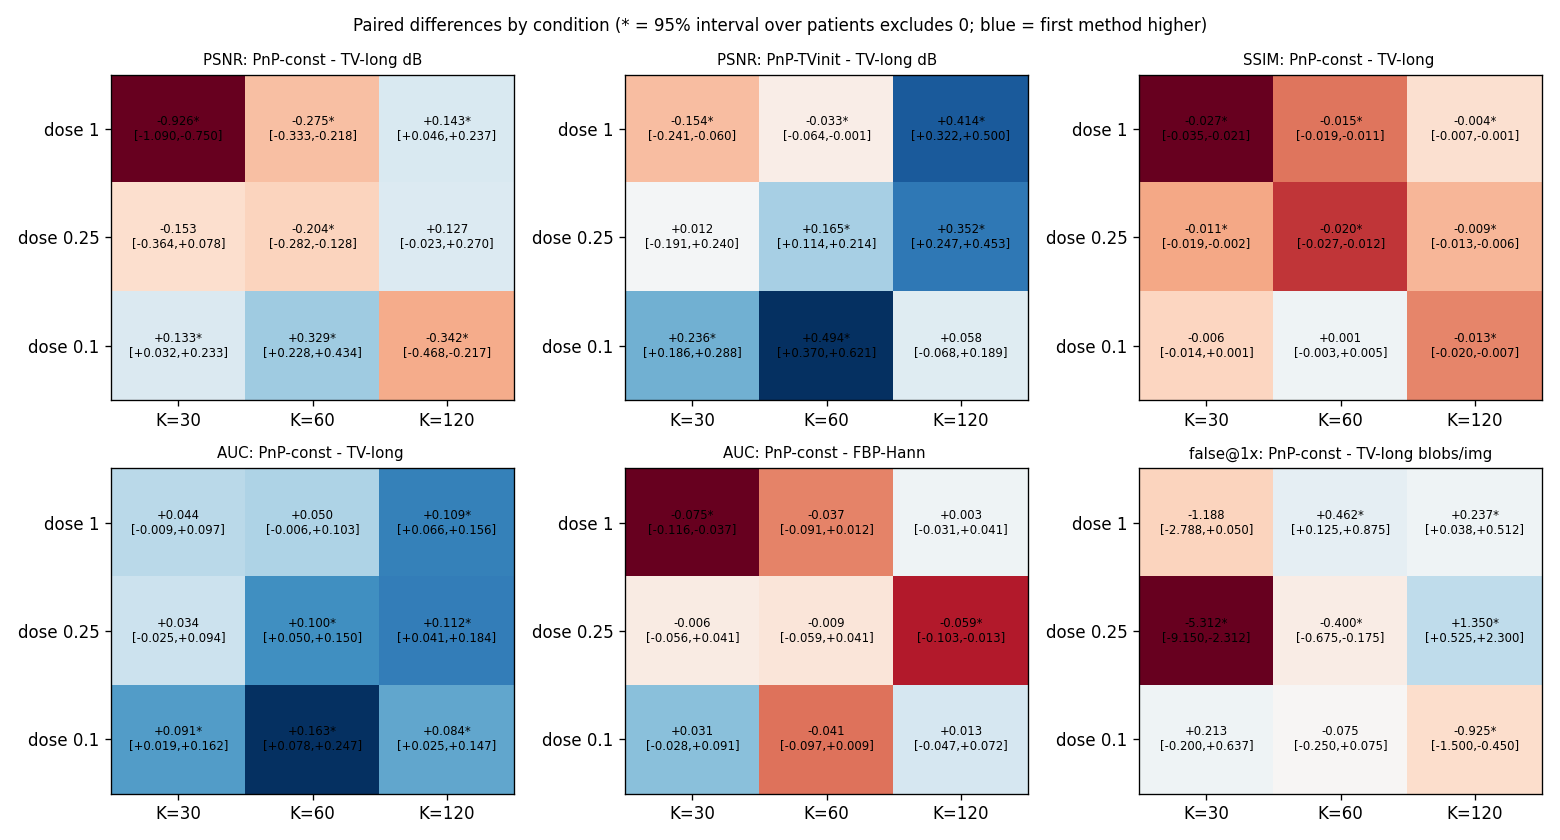
\includegraphics[width=\linewidth]{figures/step5_grid.png}
\caption{Paired differences over the nine dose $\times$ angle conditions (cell: mean, 95\% interval over 40 patients; $^*$ excludes 0; blue: the first method is higher). Top row: PSNR (PnP-const and PnP-TVinit against TV-long) and SSIM (E16); bottom row: paired AUC of PnP-const against TV-long and against FBP-Hann (E17), and the difference in false blobs per slice at one times the nominal lesion strength (E18). Produced by \texttt{run\_stage3\_step5\_summary.py}.}\label{fig:grid3}
\end{figure}

\begin{table}[htbp]
\centering\small\setlength{\tabcolsep}{3pt}
\caption{Paired AUC differences ($\sigma_l\in\{2,4\}$\,px pooled, $c=0.06$, 40 patients; mean, 95\% interval; $^*$ excludes 0).}\label{tab:det3}
\resizebox{\linewidth}{!}{%
\begin{tabular}{llccccc}
\toprule
$K$ & dose & PnP-const $-$ TV-long & PnP-const $-$ TV & PnP-const $-$ FBP-Hann & TV-long $-$ FBP-Hann & PnP-TVinit $-$ TV-long\\
\midrule
30 & 1 & $+0.044$ {\scriptsize$[{-}0.009,+0.097]$} & $+0.006$ {\scriptsize$[{-}0.050,+0.059]$} & ${-}0.075^{*}$ {\scriptsize$[{-}0.116,{-}0.037]$} & ${-}0.119^{*}$ {\scriptsize$[{-}0.169,{-}0.072]$} & $+0.066^{*}$ {\scriptsize$[+0.019,+0.113]$} \\
30 & 0.25 & $+0.034$ {\scriptsize$[{-}0.025,+0.094]$} & $+0.078^{*}$ {\scriptsize$[+0.013,+0.144]$} & ${-}0.006$ {\scriptsize$[{-}0.056,+0.041]$} & ${-}0.041$ {\scriptsize$[{-}0.103,+0.025]$} & $+0.069^{*}$ {\scriptsize$[+0.006,+0.131]$} \\
30 & 0.1 & $+0.091^{*}$ {\scriptsize$[+0.019,+0.162]$} & $+0.137^{*}$ {\scriptsize$[+0.059,+0.216]$} & $+0.031$ {\scriptsize$[{-}0.028,+0.091]$} & ${-}0.059$ {\scriptsize$[{-}0.141,+0.019]$} & $+0.053$ {\scriptsize$[{-}0.022,+0.128]$} \\
60 & 1 & $+0.050$ {\scriptsize$[{-}0.006,+0.103]$} & $+0.000$ {\scriptsize$[{-}0.050,+0.050]$} & ${-}0.037$ {\scriptsize$[{-}0.091,+0.012]$} & ${-}0.087^{*}$ {\scriptsize$[{-}0.144,{-}0.031]$} & $+0.069^{*}$ {\scriptsize$[+0.031,+0.109]$} \\
60 & 0.25 & $+0.100^{*}$ {\scriptsize$[+0.050,+0.150]$} & $+0.078^{*}$ {\scriptsize$[+0.028,+0.131]$} & ${-}0.009$ {\scriptsize$[{-}0.059,+0.041]$} & ${-}0.109^{*}$ {\scriptsize$[{-}0.175,{-}0.047]$} & $+0.084^{*}$ {\scriptsize$[+0.031,+0.141]$} \\
60 & 0.1 & $+0.163^{*}$ {\scriptsize$[+0.078,+0.247]$} & $+0.144^{*}$ {\scriptsize$[+0.072,+0.219]$} & ${-}0.041$ {\scriptsize$[{-}0.097,+0.009]$} & ${-}0.203^{*}$ {\scriptsize$[{-}0.291,{-}0.119]$} & $+0.156^{*}$ {\scriptsize$[+0.084,+0.231]$} \\
120 & 1 & $+0.109^{*}$ {\scriptsize$[+0.066,+0.156]$} & $+0.084^{*}$ {\scriptsize$[+0.044,+0.125]$} & $+0.003$ {\scriptsize$[{-}0.031,+0.041]$} & ${-}0.106^{*}$ {\scriptsize$[{-}0.162,{-}0.053]$} & $+0.091^{*}$ {\scriptsize$[+0.050,+0.137]$} \\
120 & 0.25 & $+0.112^{*}$ {\scriptsize$[+0.041,+0.184]$} & $+0.081^{*}$ {\scriptsize$[+0.006,+0.156]$} & ${-}0.059^{*}$ {\scriptsize$[{-}0.103,{-}0.013]$} & ${-}0.172^{*}$ {\scriptsize$[{-}0.247,{-}0.094]$} & $+0.166^{*}$ {\scriptsize$[+0.109,+0.222]$} \\
120 & 0.1 & $+0.084^{*}$ {\scriptsize$[+0.025,+0.147]$} & $+0.084^{*}$ {\scriptsize$[+0.028,+0.147]$} & $+0.013$ {\scriptsize$[{-}0.047,+0.072]$} & ${-}0.072^{*}$ {\scriptsize$[{-}0.128,{-}0.016]$} & $+0.022$ {\scriptsize$[{-}0.041,+0.081]$} \\
\bottomrule
\end{tabular}}
\end{table}


\subsection{E18: False structures on real slices}\label{sec:e18}
Table~\ref{tab:absfb3} (CT rows) gives the mean number of false blobs per lesion-free slice at one times the nominal lesion strength for the four conditions that are also used in the shift study. A false blob is defined in Section~\ref{sec:observer3}; because the ground truth of LoDoPaB-CT is itself a reconstruction, ``false'' means unsupported by this reference and not absent from the patient.
On real slices PnP-const makes $0.24$--$1.38$ such blobs per slice and TV-long $0.00$--$6.06$ (FBP-Hann $5.8$--$26.8$), so the regularised methods make far fewer than FBP-Hann, but the counts of TV-long are not small in every condition.
Over the nine conditions the paired difference PnP-const $-$ TV-long at $m=1$ (Table~\ref{tab:fb3}) is significantly positive in three ($K=60$ full dose: $+0.46$; $K=120$ full and quarter dose: $+0.24$, $+1.35$), significantly negative in three ($K=30$ quarter dose: $-5.31$; $K=60$ quarter dose: $-0.40$; $K=120$ dose 0.1: $-0.93$) and not significant in three, with no consistent pattern in dose or angle count: at $K=120$ the sign changes from positive to negative as the dose decreases, at $K=30$ it is negative in two of three conditions.
At $m=1.5$ the excess of PnP-const over TV-long is at most $0.45$ blobs per slice ($K=120$, quarter dose). In the $K=60$ experiment (E17b, threshold $m=0.5$) PnP-const has fewer false blobs than TV at both doses ($-1.7$ at full dose, $-6.6$ at quarter dose). Counts are not comparable with E9: there the lesion-free images are digits on an empty background and the learned prior produced essentially none in distribution, whereas here the background is real anatomy, which contains many structures of lesion size.

The galleries of the strongest unsupported blob per slice (Figures~\ref{fig:gal1} and~\ref{fig:gal025}) show that the largest false blobs occur at the same location in FBP-Hann and in TV as well as in PnP (for example the slices 28 and 9 at full dose and most rows at quarter dose), so they are produced by the data (few views, noise, streaks), not by the prior. Only a few look specific to the prior: a crescent in slice 18 at full dose
(PnP-const only) and streaks in the PnP-TVinit image of slice 32 at quarter dose. We therefore find \emph{no evidence that the prior creates many lesion-like structures in distribution}, but we cannot exclude rare ones: 40 slices and one noise draw per condition do not bound a rare event, and the galleries show the worst cases selected by the methods' own responses, not a random sample.

\begin{table}[htbp]
\centering\small\setlength{\tabcolsep}{3pt}
\caption{Paired differences in false blobs per lesion-free slice on real CT slices (40 patients; mean, 95\% interval; $^*$ excludes 0), pooled over $\sigma_l\in\{2,4\}$; $m$: threshold in units of the nominal lesion response.}\label{tab:fb3}
\resizebox{\linewidth}{!}{%
\begin{tabular}{llccc}
\toprule
$K$ & dose & $m=1$: PnP-const $-$ TV-long & $m=1$: PnP-const $-$ TV & $m=1.5$: PnP-const $-$ TV-long\\
\midrule
30 & 1 & ${-}1.19$ {\scriptsize$[{-}2.79,+0.05]$} & ${-}0.54$ {\scriptsize$[{-}1.57,+0.36]$} & ${-}0.23$ {\scriptsize$[{-}0.64,+0.11]$} \\
30 & 0.25 & ${-}5.31^{*}$ {\scriptsize$[{-}9.15,{-}2.31]$} & ${-}4.81^{*}$ {\scriptsize$[{-}8.41,{-}2.00]$} & ${-}2.42^{*}$ {\scriptsize$[{-}4.56,{-}0.82]$} \\
30 & 0.1 & $+0.21$ {\scriptsize$[{-}0.20,+0.64]$} & $+0.31$ {\scriptsize$[{-}0.12,+0.76]$} & $+0.00$ {\scriptsize$[{-}0.14,+0.14]$} \\
60 & 1 & $+0.46^{*}$ {\scriptsize$[+0.12,+0.88]$} & $+0.19^{*}$ {\scriptsize$[+0.01,+0.40]$} & $+0.12^{*}$ {\scriptsize$[+0.03,+0.25]$} \\
60 & 0.25 & ${-}0.40^{*}$ {\scriptsize$[{-}0.68,{-}0.17]$} & ${-}0.60^{*}$ {\scriptsize$[{-}1.11,{-}0.19]$} & ${-}0.11^{*}$ {\scriptsize$[{-}0.25,{-}0.01]$} \\
60 & 0.1 & ${-}0.07$ {\scriptsize$[{-}0.25,+0.07]$} & ${-}0.05$ {\scriptsize$[{-}0.20,+0.09]$} & ${-}0.01$ {\scriptsize$[{-}0.06,+0.04]$} \\
120 & 1 & $+0.24^{*}$ {\scriptsize$[+0.04,+0.51]$} & $+0.11^{*}$ {\scriptsize$[+0.01,+0.25]$} & $+0.06$ {\scriptsize$[+0.00,+0.15]$} \\
120 & 0.25 & $+1.35^{*}$ {\scriptsize$[+0.53,+2.30]$} & $+1.35^{*}$ {\scriptsize$[+0.54,+2.29]$} & $+0.45^{*}$ {\scriptsize$[+0.16,+0.81]$} \\
120 & 0.1 & ${-}0.93^{*}$ {\scriptsize$[{-}1.50,{-}0.45]$} & ${-}0.88^{*}$ {\scriptsize$[{-}1.48,{-}0.39]$} & ${-}0.11^{*}$ {\scriptsize$[{-}0.26,{-}0.01]$} \\
\bottomrule
\end{tabular}}
\end{table}

\begin{figure}[p]
\centering
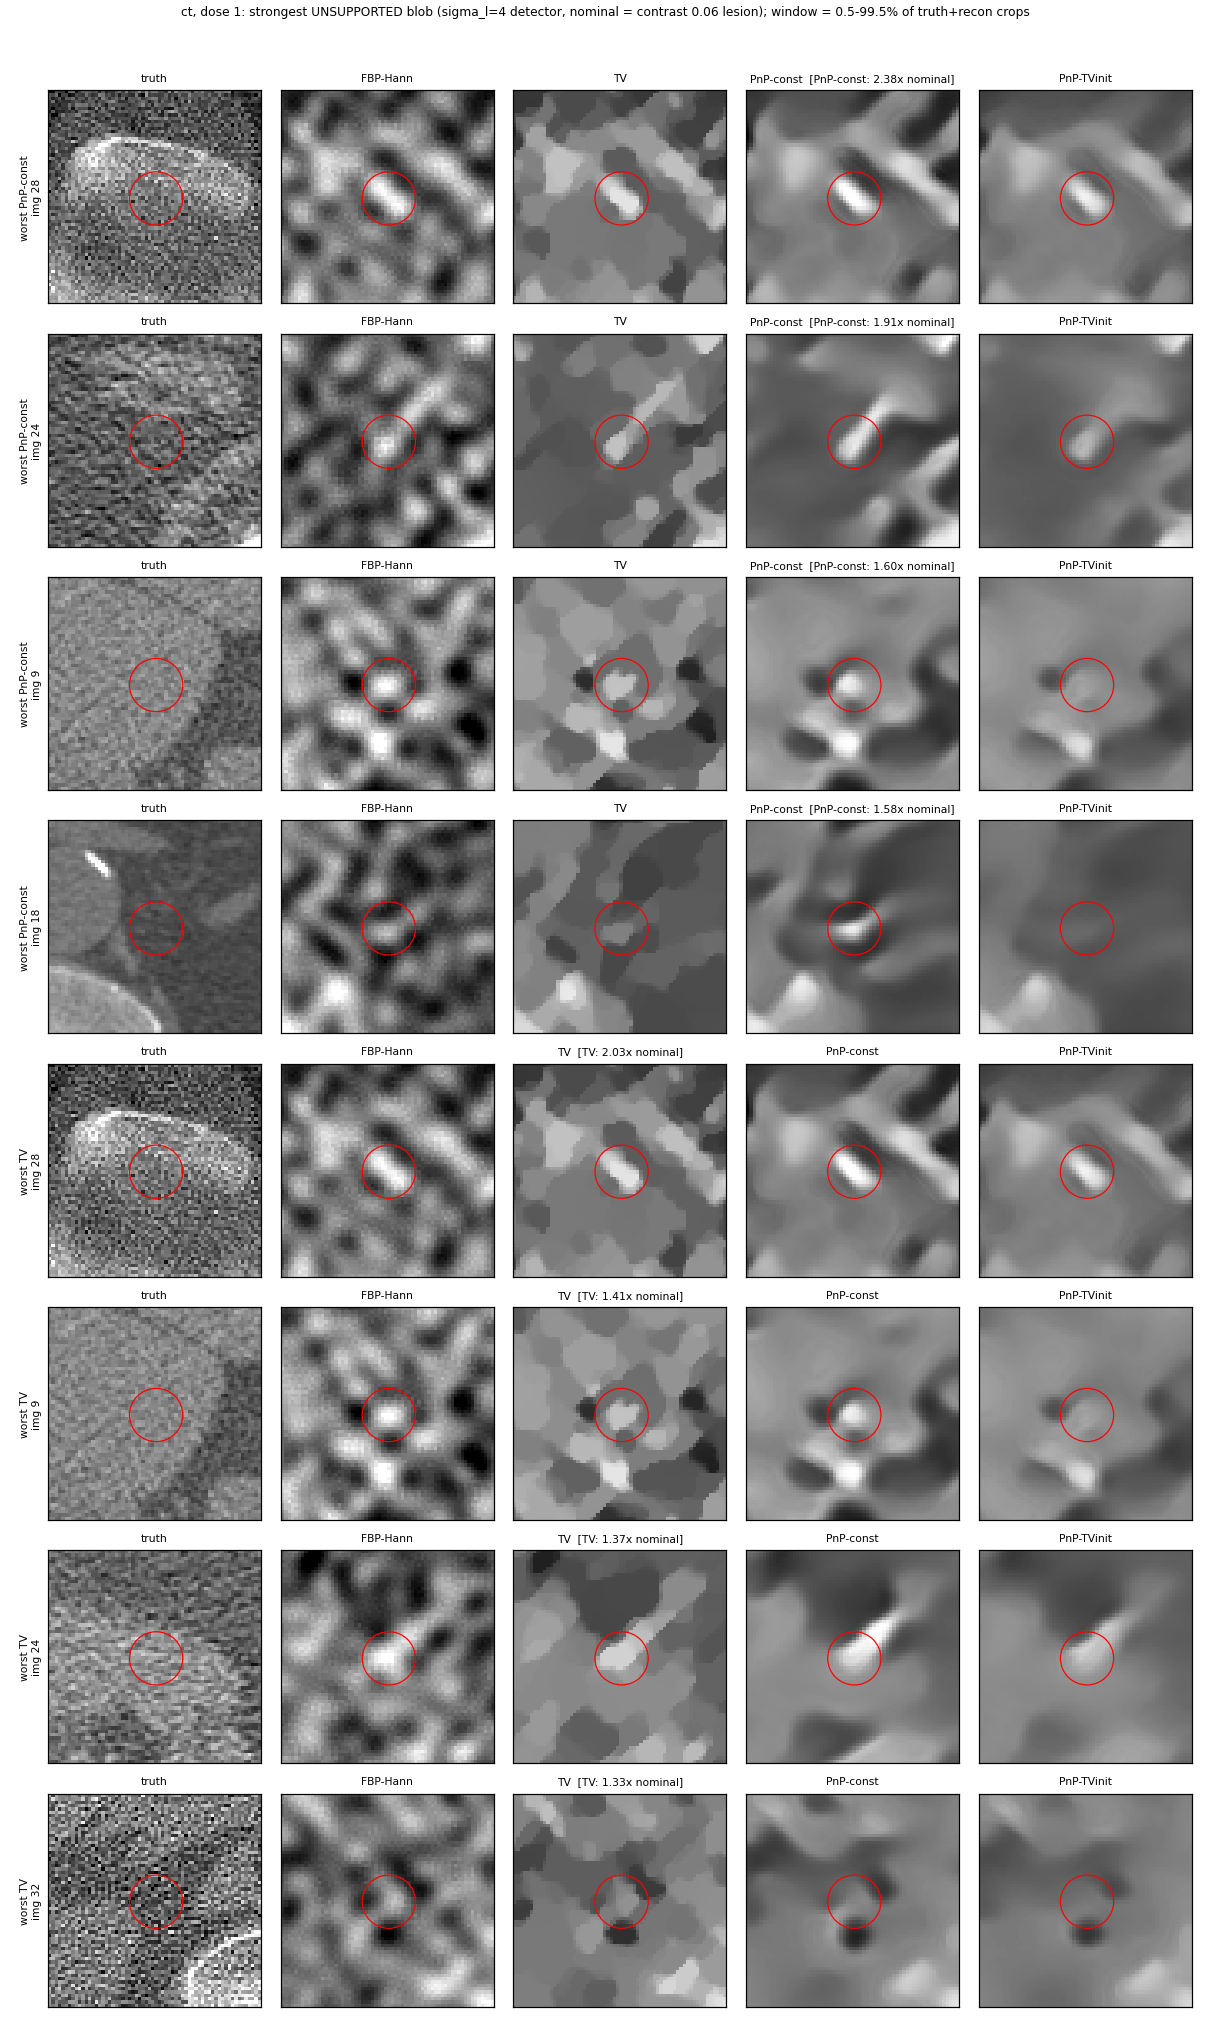
\includegraphics[height=0.9\textheight,keepaspectratio]{figures/step4b_gallery_ct_dose1.png}
\caption{Strongest unsupported blob per slice at full dose ($K=60$; $\sigma_l=4$\,px detector) for the four slices with the largest false-blob response in PnP-const (top four rows) and in TV (bottom four rows). Columns: ground truth crop, FBP-Hann, TV, PnP-const, PnP-TVinit; red circle: location of the blob; labels give the response as a multiple of the nominal lesion response.}\label{fig:gal1}
\end{figure}

\begin{figure}[p]
\centering
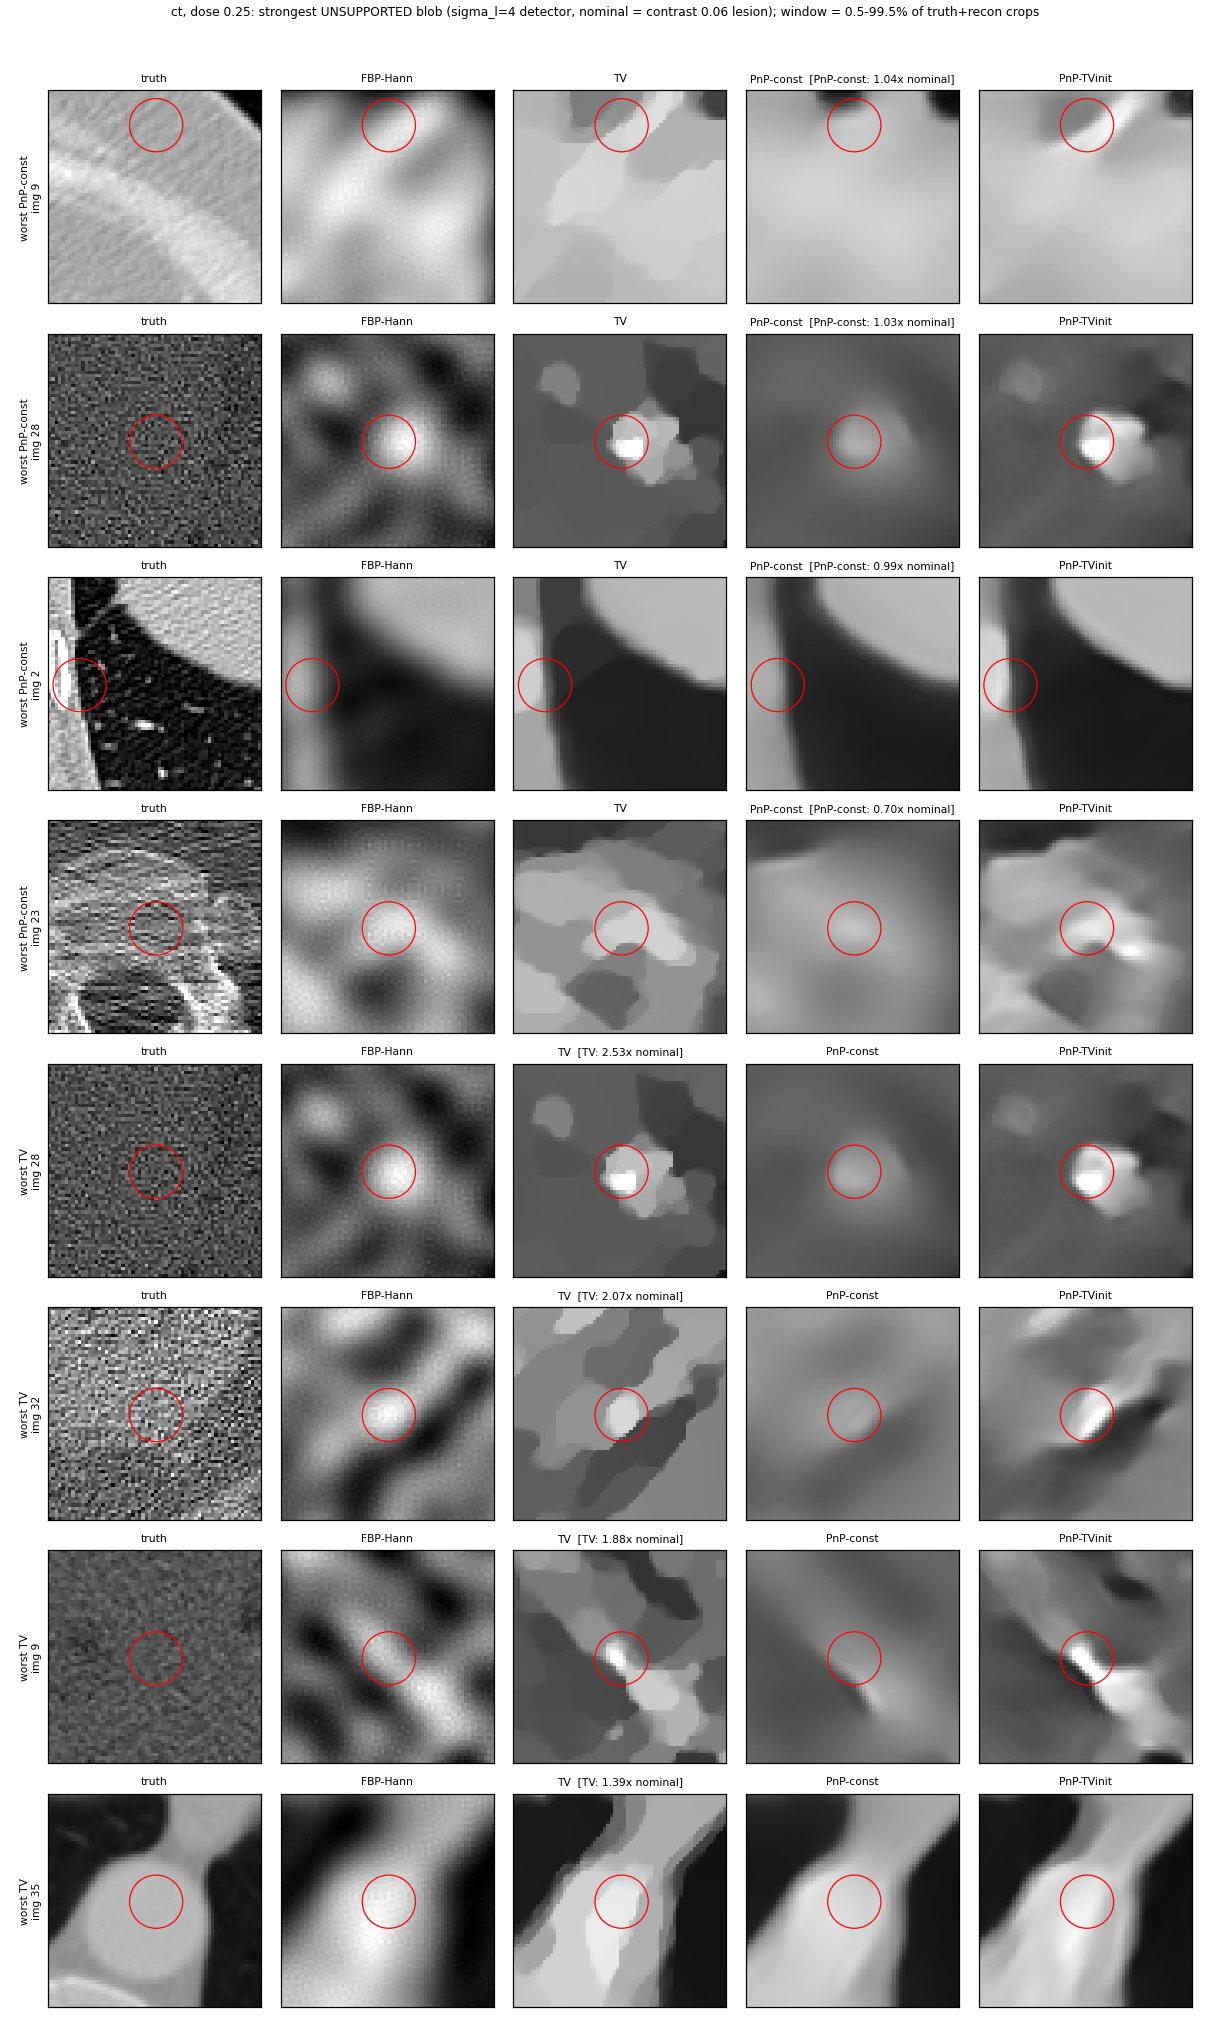
\includegraphics[height=0.9\textheight,keepaspectratio]{figures/step4b_gallery_ct_dose0.25.png}
\caption{As Figure~\ref{fig:gal1} at quarter dose.}\label{fig:gal025}
\end{figure}


\subsection{E19: Distribution shift to non-anatomical phantoms}\label{sec:e19}
The CT-trained prior and all tuned parameters are applied, without retuning, to 20 random piecewise-constant phantoms (ellipses, rectangles and a stripe or checker block on a faint disc, $\mu/\mu_{\max}$ scale; nothing like a CT slice, but the kind of image TV favours; same phantoms in every condition; this is a deliberately TV-friendly shift, so it tests how much of the learned prior's behaviour survives, not how it fares under realistic shifts such as another scanner or anatomy) with the same lesion protocol. The shift was first run at $K=60$ (doses 1 and 0.25) and
then extended to $K=30$ and $120$; the $K=60$ analysis used four lesion types, the others two, so the designs differ slightly.
 
\emph{Accuracy and detection (Table~\ref{tab:shift3a}).} On the phantoms PnP-const is below TV-long in PSNR in all six conditions ($-0.11$ to $-0.75$\,dB; significantly in five of the six conditions, the exception being $K=30$, full dose) and in SSIM in all four ($-0.095$ to $-0.190$, all significant, against $-0.004$ to $-0.027$ on CT).
At quarter dose its SSIM is also below FBP-Hann's on the phantoms ($-0.045$ at $K=30$ and $-0.041$ at $K=120$, both significant). The detection advantage over TV-long is significant in one of six shift conditions ($K=120$, full dose: $+0.075$, $[+0.013,+0.137]$), against three of the six corresponding CT conditions ($K=60$ quarter dose, $K=120$ at both doses);
the shift effect is significantly negative only at $K=120$, quarter dose ($-0.175$, $[-0.297,-0.056]$). The CT advantage is therefore not reliably transferred to the shifted images, but at 20 phantoms the interval widths of $0.12$--$0.19$ do not allow us to say that it is lost either.
In PSNR the shift costs at most about $0.75$\,dB against TV-long, much less than the $3$--$4$\,dB reversals of the $28\times28$ experiments (E4, E8); in SSIM the deficit is large ($-0.095$ to $-0.190$).
 
\emph{False blobs (Tables~\ref{tab:shift3a}--\ref{tab:absfb3}).} The sign of PnP-const $-$ TV at $1\times$ lesion strength follows the number of angles: negative (or not different from zero) at $K=30$ and negative at full-dose $K=60$, mixed at $K=60$ quarter dose ($\sigma_l=2$: $-7.5$; $\sigma_l=4$: $+9.1$), and positive at $K=120$ ($+9.0$ to $+13.0$ per phantom at both doses; at $1.5\times$ against TV-long $+10.2$ at full dose and $+3.8$ at quarter dose, both significant).
The absolute counts show why (Table~\ref{tab:absfb3}): the count of TV-long varies from $3.2$ to $83.9$ per phantom over the four conditions, that of PnP-const only from $12.8$ to $50.3$; at $K=30$ TV-long makes two to three times as many false blobs as FBP-Hann ($30.2$ vs.\ $15.5$ at quarter dose, $83.9$ vs.\ $31.6$ at full dose), at $K=120$ about a third or less ($3.2$ vs.\ $8.7$, i.e.\ $37\%$; $32.1$ vs.\ $118.7$, i.e.\ $27\%$).
So the ``excess'' of PnP-const at $K=120$ is relative to a TV that is unusually clean there. Relative to \emph{FBP-Hann} the picture is more informative: at full dose PnP-const has fewer false blobs on the phantoms ($-7.1$ at $K=30$, $-68.4$ at $K=120$, both significant), but at quarter dose it has more at both $K$ ($+1.0$, not significant, and $+4.0$ [$+2.4,+5.9$] at $1\times$;
$+2.2$ [$+1.1,+3.4$] and $+2.7$ [$+1.4,+4.4$] at $1.5\times$), in contrast to real slices, where it has significantly fewer than FBP-Hann in both quarter-dose conditions ($-9.0$ and $-4.4$). In this sense the shift turns the prior from suppressing to adding false blobs relative to the unregularised reconstruction at quarter dose, by a few blobs per phantom, although this is significant only at $K=120$. The pooled counts hide a dependence on lesion size: at $1\times$, for $\sigma_l=2$ PnP-const has more false blobs than FBP-Hann on the phantoms in three of the four conditions ($+10.1$, $+9.7$ and $+10.6$ at $K=30$ full and quarter dose and $K=120$ quarter dose, all significant), for $\sigma_l=4$ fewer in all four ($-24.3$, $-7.7$, $-30.9$, $-2.5$).
At $K=120$, full dose, PnP-TVinit with almost no denoising ($\sigma_d=0.0039$) also produces $14.0$ more blobs than TV-long ($[+7.4,+22.0]$ at $1\times$, for all $\sigma_l$), so at least part of the excess at $K=120$ is not due to the denoiser; we did not isolate the cause.
In the gallery of the strongest unsupported blob per phantom (Figure~\ref{fig:galshape}, $K=60$, quarter dose) the worst blobs again occur at the same location in FBP-Hann, TV and PnP, mostly in uniform regions of the phantom, with TV reaching up to $4.9$ times the nominal lesion response and the four worst PnP-const blobs between about $2.8$ and $3.2$ times; in these examples the prior does not create blobs that the data do not already suggest.
 
\begin{table}[htbp]
\centering\small\setlength{\tabcolsep}{3pt}
\caption{Distribution shift to phantoms (20 phantoms; mean, 95\% interval; $^*$ excludes 0). Left: false blobs per phantom at $1\times$ lesion strength, PnP-const $-$ TV, by lesion size. Right: PnP-const $-$ TV-long on the phantoms: pooled paired AUC, PSNR (dB) and SSIM.
$K=60$ rows: AUC from four lesion types (E17b), PSNR interval from a bootstrap over the 20 phantoms (\texttt{run\_e19\_k60\_psnr\_ci.py}), SSIM not stored.}\label{tab:shift3a}
\resizebox{\linewidth}{!}{%
\begin{tabular}{llcccccc}
\toprule
 & & \multicolumn{2}{c}{false blobs, $1\times$} & & & & \\
\cmidrule(lr){3-4}
$K$ & dose & $\sigma_l=2$ & $\sigma_l=4$ & AUC & PSNR & SSIM\\
\midrule
30 & 1 & ${-}70.7^{*}$ {\scriptsize$[{-}107.0,{-}38.7]$} & ${-}31.8^{*}$ {\scriptsize$[{-}48.7,{-}16.8]$} & ${-}0.037$ {\scriptsize$[{-}0.113,+0.037]$} & ${-}0.11$ {\scriptsize$[{-}0.37,+0.18]$} & ${-}0.095^{*}$ {\scriptsize$[{-}0.125,{-}0.063]$} \\
30 & 0.25 & ${-}21.1^{*}$ {\scriptsize$[{-}34.3,{-}10.3]$} & ${-}1.8$ {\scriptsize$[{-}5.8,+1.8]$} & $+0.056$ {\scriptsize$[{-}0.031,+0.144]$} & ${-}0.53^{*}$ {\scriptsize$[{-}0.64,{-}0.40]$} & ${-}0.190^{*}$ {\scriptsize$[{-}0.204,{-}0.172]$} \\
60 & 1 & ${-}20.1^{*}$ {\scriptsize$[{-}34.4,{-}7.6]$} & ${-}6.5^{*}$ {\scriptsize$[{-}12.6,{-}1.4]$} & ${-}0.019$ {\scriptsize$[{-}0.06,+0.02]$} & ${-}0.30^{*}$ {\scriptsize$[{-}0.44,{-}0.14]$} & n/a \\
60 & 0.25 & ${-}7.5^{*}$ {\scriptsize$[{-}12.9,{-}2.8]$} & $+9.1^{*}$ {\scriptsize$[+6.0,+12.8]$} & $+0.050$ {\scriptsize$[{-}0.01,+0.11]$} & ${-}0.75^{*}$ {\scriptsize$[{-}0.82,{-}0.67]$} & n/a \\
120 & 1 & $+13.0^{*}$ {\scriptsize$[+8.8,+17.5]$} & $+9.2^{*}$ {\scriptsize$[+5.4,+13.2]$} & $+0.075^{*}$ {\scriptsize$[+0.013,+0.137]$} & ${-}0.51^{*}$ {\scriptsize$[{-}0.56,{-}0.45]$} & ${-}0.179^{*}$ {\scriptsize$[{-}0.190,{-}0.168]$} \\
120 & 0.25 & $+10.4^{*}$ {\scriptsize$[+5.9,+16.0]$} & $+9.0^{*}$ {\scriptsize$[+5.9,+12.3]$} & ${-}0.062$ {\scriptsize$[{-}0.162,+0.031]$} & ${-}0.62^{*}$ {\scriptsize$[{-}0.68,{-}0.57]$} & ${-}0.155^{*}$ {\scriptsize$[{-}0.162,{-}0.149]$} \\
\bottomrule
\end{tabular}}
\end{table}
 
\begin{table}[htbp]
\centering\small\setlength{\tabcolsep}{4pt}
\caption{Mean false blobs per lesion-free image at $1\times$ nominal lesion strength (mean of $\sigma_l=2$ and $4$) on real CT slices and on the phantoms, and PnP-const $-$ FBP-Hann (mean, 95\% interval over patients or phantoms).}\label{tab:absfb3}
\begin{tabular}{llcccccc}
\toprule
set & $K$, dose & FBP-Hann & TV & TV-long & PnP-const & PnP-TVinit & PnP-const $-$ FBP\\
\midrule
CT     & 30, 0.25  & 9.78 & 5.56 & 6.06 & 0.75 & 0.64 & $-9.03^{*}$ {\scriptsize$[-13.21,-5.20]$}\\
CT     & 30, 1     & 5.78 & 1.04 & 1.69 & 0.50 & 0.32 & $-5.28^{*}$ {\scriptsize$[-7.54,-3.29]$}\\
CT     & 120, 0.25 & 5.79 & 0.02 & 0.02 & 1.38 & 0.39 & $-4.41^{*}$ {\scriptsize$[-7.34,-2.00]$}\\
CT     & 120, 1    & 26.79 & 0.12 & 0.00 & 0.24 & 0.18 & $-26.55^{*}$ {\scriptsize$[-43.93,-12.63]$}\\
phantom & 30, 0.25  & 15.48 & 27.95 & 30.20 & 16.50 & 11.65 & $+1.03$ {\scriptsize$[-0.68,+2.75]$}\\
phantom & 30, 1     & 31.60 & 75.72 & 83.90 & 24.48 & 57.30 & $-7.13^{*}$ {\scriptsize$[-10.68,-4.02]$}\\
phantom & 120, 0.25 & 8.72 & 3.08 & 3.18 & 12.75 & 11.48 & $+4.03^{*}$ {\scriptsize$[+2.35,+5.90]$}\\
phantom & 120, 1    & 118.68 & 39.20 & 32.08 & 50.30 & 46.12 & $-68.38^{*}$ {\scriptsize$[-92.68,-45.23]$}\\
\bottomrule
\end{tabular}
\end{table}

\begin{figure}[p]
\centering
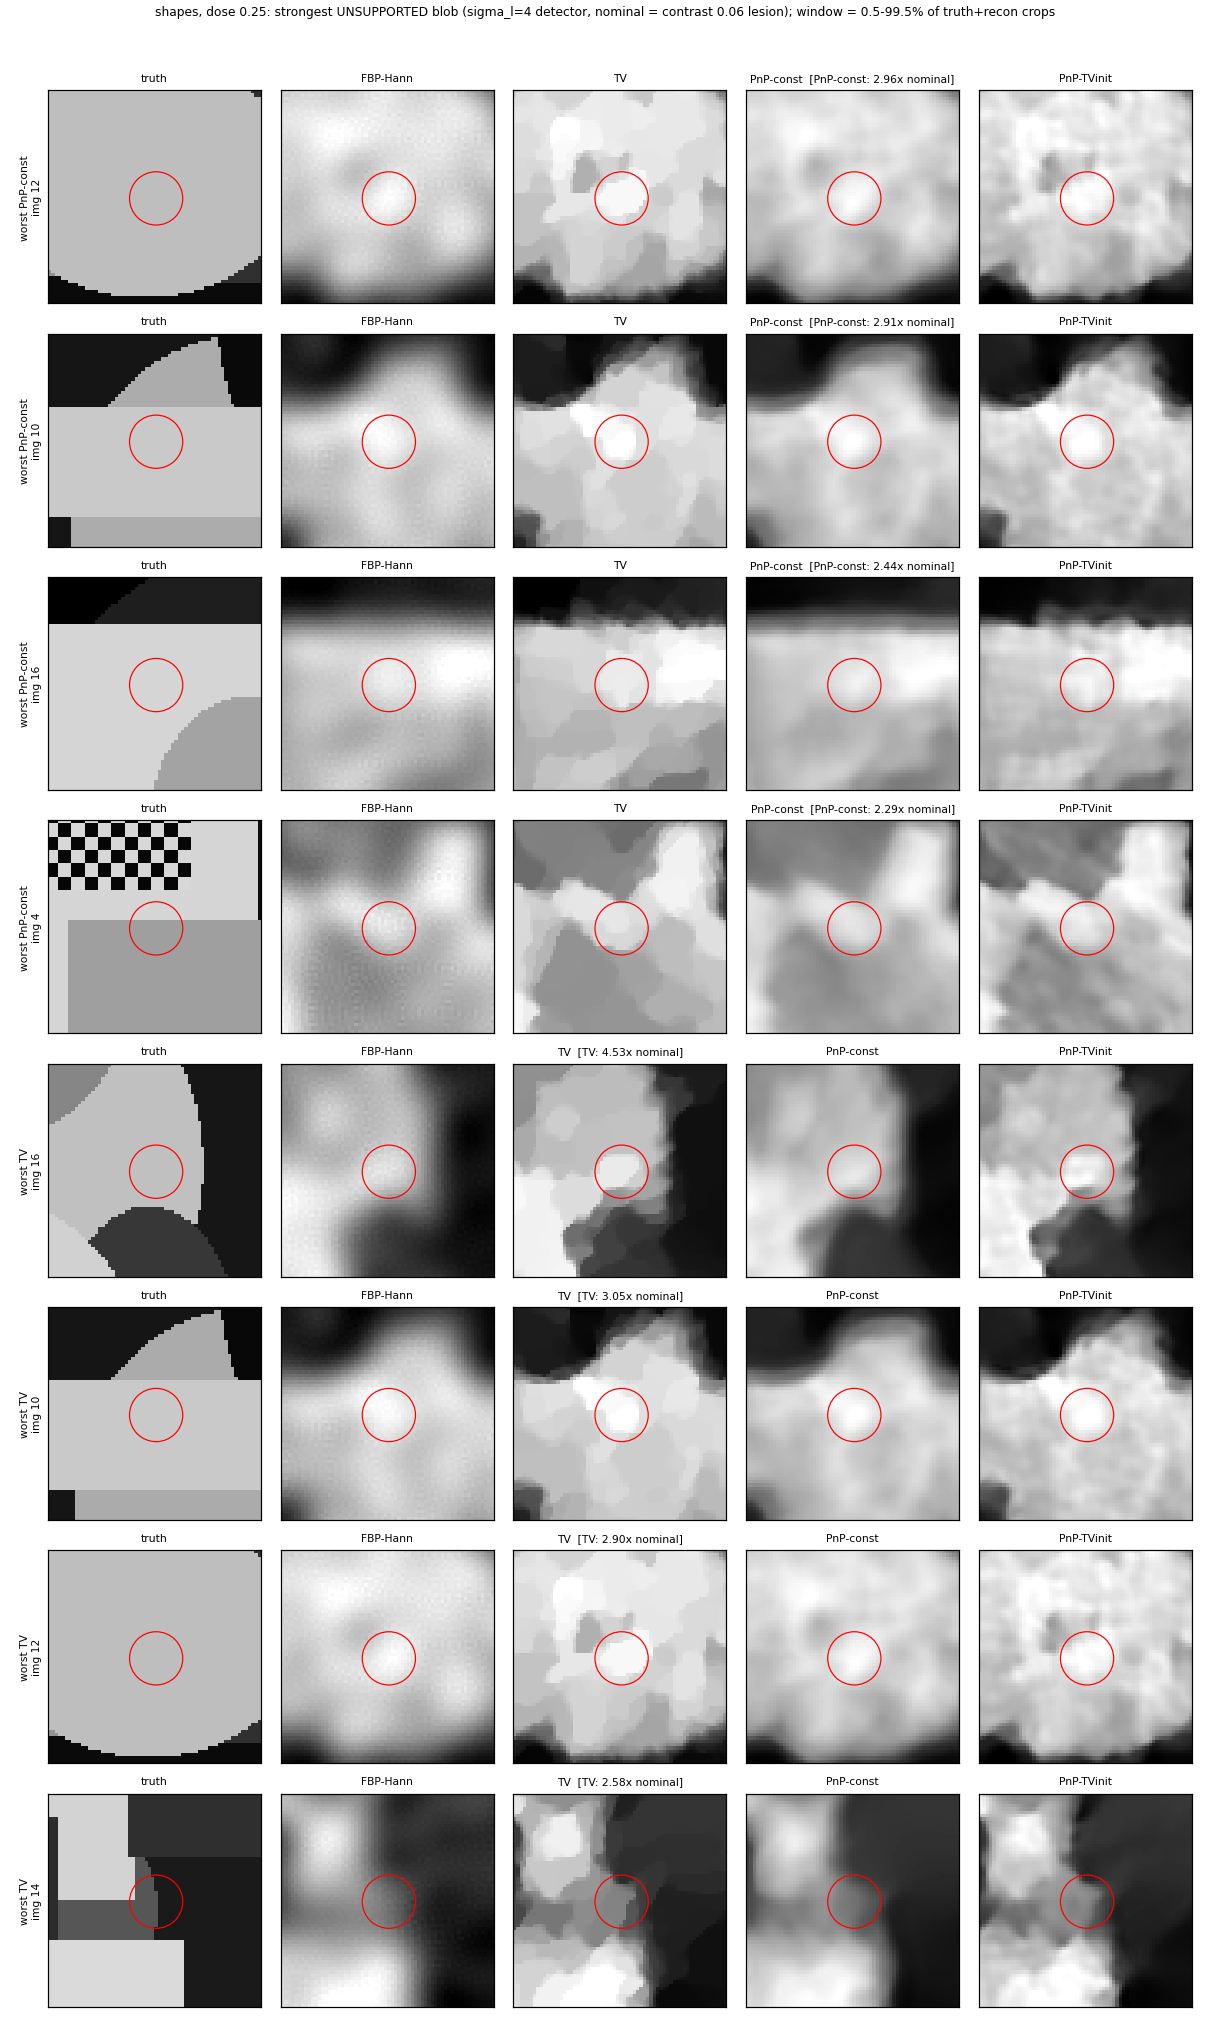
\includegraphics[height=0.9\textheight,keepaspectratio]{figures/step4b_gallery_shapes_dose0.25.png}
\caption{Strongest unsupported blob per phantom at quarter dose ($K=60$; $\sigma_l=4$\,px detector) for the four phantoms with the largest false-blob response in PnP-const (top four rows) and in TV (bottom four rows). Columns: ground truth crop, FBP-Hann, TV, PnP-const, PnP-TVinit; red circle: location of the blob; labels give the response as a multiple of the nominal lesion response.}\label{fig:galshape}
\end{figure}
